\chapter{Continuous Toolpath Planning in Additive Manufacturing}

\section{Introduction} \label{sec:introadditiv}

\emph{Additive manufacturing} refers to any process that adds material  to create a 3D object. %
3D printing is a popular form of additive manufacturing that deposits material (plastic, metal, biomaterial, polymer, etc.) in layer by layer fashion. % to form the object.
We focus on extrusion based 3D printing, in which material is pushed out of an extruder that follows some tool path while depositing material in beads that meld together upon contact.
In this paper, we will refer to this process simply as 3D printing.


In most 3D printing jobs, we first print the outer ``shell'' or boundary of the 3D object in each layer.
We then cover the interior space by printing an \emph{infill lattice} \cite{WuAaWeSi2018}, which is typically a standard mesh. % \cite{BrBrWiHa2012},
In an arbitrary infill lattice, one is not guaranteed to find a \emph{continuous} tool path, i.e., an entire layer being printed by non-stop extrusion of material.
Non-continuous tool paths typically have multiple starts and stops, which could reduce quality of the print, cause print failures (e.g., delamination), and could increase print time.
To ensure existence of a continuous tool path, we need to choose the mesh modeling the infill lattice carefully.
Subsequently, we need to develop algorithms that ensure a continuous tool path can be obtained for each layer with arbitrary geometry.
Further, we need to identify a traversel of this tool path that avoids crossovers.
%We propose an approach to transform any cellular complex under mild assumptions into an \emph{Eulerian} complex.
%Every vertex in the $1$-skeleton (i.e., graph) of an Eulerian complex has an even degree, and hence a continuous tool path is guaranteed to exist.

\subsection{Our contributions} \label{ssec:contribaddit}
We recently proposed a method that transforms a given $2$-dimensional cell complex $K$ into a new $2$-complex $\hK$ in which every vertex is part of a uniform even number of edges \cite{GuKr2018}.
Hence every vertex in the graph $\hG$ that is the $1$-skeleton of $\hK$ has an even degree, which makes $\hG$ Eulerian, i.e., it is guaranteed to contain an Eulerian tour.
We refer to this method as an \emph{Euler transformation} of a polygonal (or cell) complex.
%We first describe the Euler transformation of a $2$-complex \emph{abstractly}.
For the sake of completeness of the present paper, we present details of the Euler transformation in 2D here.
For $2$-complexes in $\R^2$ under mild assumptions (that no two adjacent edges of a polygon in $K$ are boundary edges), we show that the Euler transformed $2$-complex $\hK$ has a geometric realization in $\R^2$, and that each vertex in its $1$-skeleton has degree $4$.
We bound the numbers of vertices, edges, and polygons in $\hK$ as small scalar multiples of the corresponding numbers in $K$.
\begin{comment}
We prove corresponding results for $3$-complexes in $\R^3$ under an additional assumption that each vertex in $K$ is connected to three edges in a $3$-cell that contains the vertex, i.e., the degree of each vertex in the $1$-skeleton of each $3$-cell in $K$ containing the vertex is $3$.
In this setting, every vertex in $\hG$ is shown to have a degree of $6$.
Next, we presents bounds on parameters measuring geometric quality (aspect ratios) of $\hK$ in terms of the corresponding parameters of $K$ (for $d=2$).
One can control these quality measures by choosing user-defined offset parameters appropriately.
\end{comment}

We present a computational framework for 3D printing that identifies continuous tool paths for printing the infill lattice in each layer. We illustrate the steps in our framework in Figure \ref{infill_pattern_work_flow} (on a 3D pyramid with a square base).
First we find the polygons for each layer of the input 3D domain (typically presented as an STL file, e.g., Figure \ref{pyramid})) using a slicing software.
Let $\Ps$ be the union of all of these polygons in 2D (Figure \ref{union_of_projections}). 
We fill the space in $\Ps$ with some infill lattice $K$, using any meshing algorithm (Figure \ref{infill_pattern}).
We then apply Euler transformation to obtain a new infill lattice $\hK$ that is guaranteed to be Euler (Figure \ref{infill_pattern_transformed}).
In the next step, we \emph{clip} $\hK$ using $P_i$, a polygon in layer $i$ (Figure \ref{infill_pattern_transformed_polygon_cut}).
Depending on the shape of $P_i$, this step could create terminal vertices in the infill lattice for layer $i$, making it no longer Euler.
In the last step, we \emph{patch} the clipped infill lattice by adding new edges such that the resulting infill lattice is Euler again (Figure \ref{infill_pattern_transformed_polygon_patch_simple}).
An application of this framework is illustrated in Figures \ref{pyramidplan} and \ref{printedpyramid}.
Finally, we propose a tool path algorithm (Section \ref{sec:toolpathalgo}) that identifies the actual print tool path from the patched Euler infill lattice that avoids crossovers and material collisions.
We address all geometric/computational challenges that arise along the way to ensure the proposed framework is complete.
Since each layer can have multiple polygons in general, our framework can generate continuous tool path for each polygon in a given layer (see Section \ref{sec:boundaryedges} for an exception arising in certain cases with extreme geometries).
As we might not print every boundary edge after the patching step, we also print \emph{support} edges (see Section \ref{sec:slicing}).
The overall goal of our framework is to create an Euler infill lattice in each layer, and also prevent printing in free space so as to avoid print failures.
We are currently investigating the implementation and testing of our algorithmic framework for 3D printing in detail, and plan to present details in an uncoming paper.

\begin{figure}[htp!]
  \centering
%\hspace*{0.15in}
  \begin{subfigure}[t]{1.7in}
    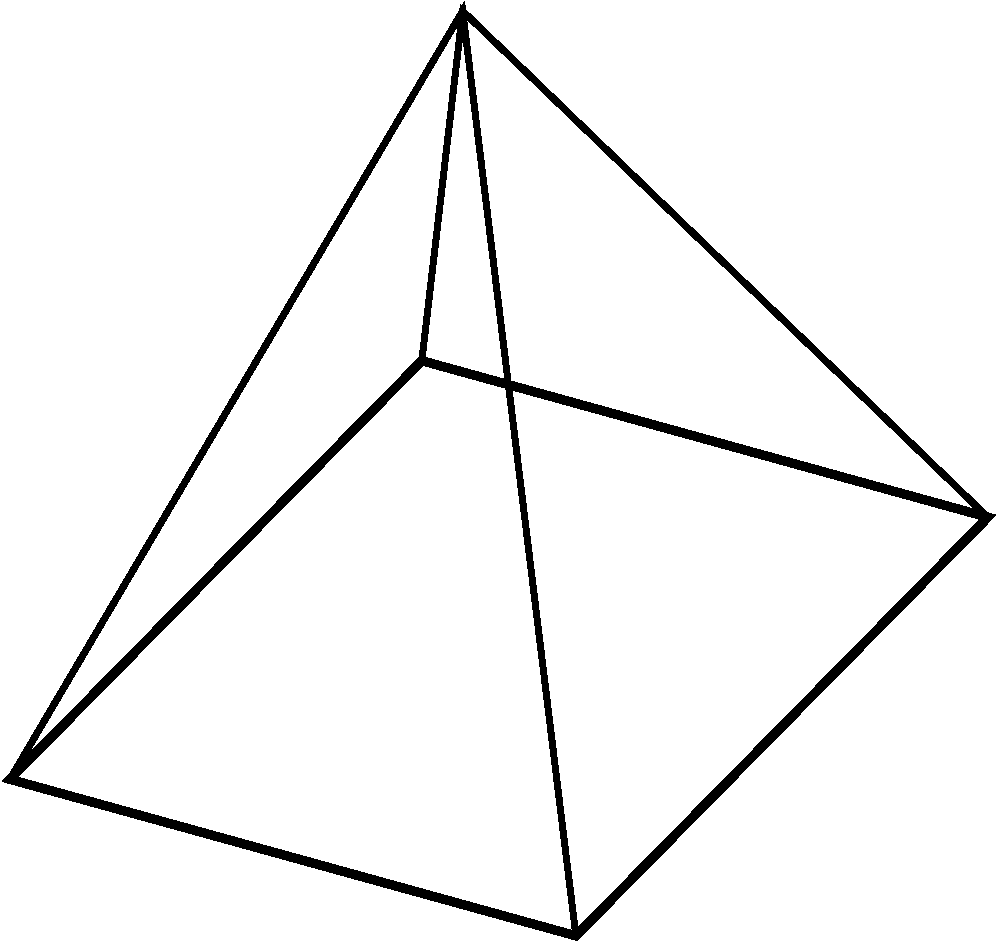
\includegraphics[scale=0.25]{pyramid_crop}
    \caption{\small \label{pyramid}}
  \end{subfigure}
%\hspace*{0.15in}
  \begin{subfigure}[t]{1.7in}
    
\includegraphics[scale=0.25]{union_of_projections_crop}
    \caption{\small \label{union_of_projections}}
  \end{subfigure}
%\hspace*{0.15in}
  \begin{subfigure}[t]{1.7in}
    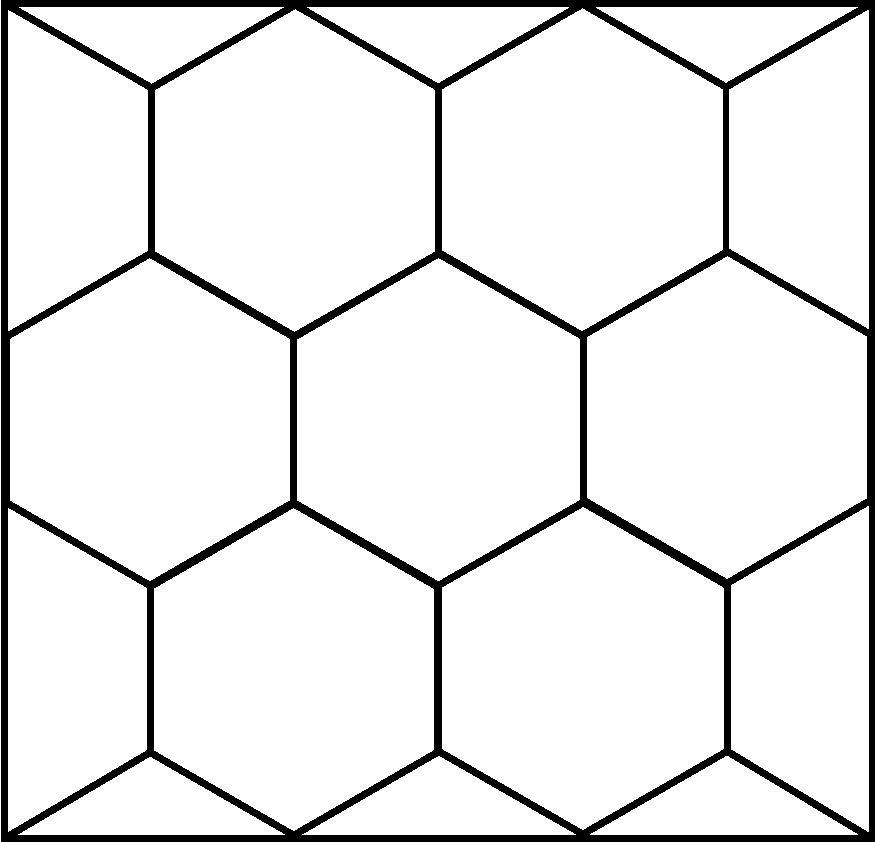
\includegraphics[scale=0.25]{infill_pattern_crop}
    \caption{\small \label{infill_pattern}}
  \end{subfigure}
%\hspace*{0.15in}
  \begin{subfigure}[t]{1.7in}
    %\centering
    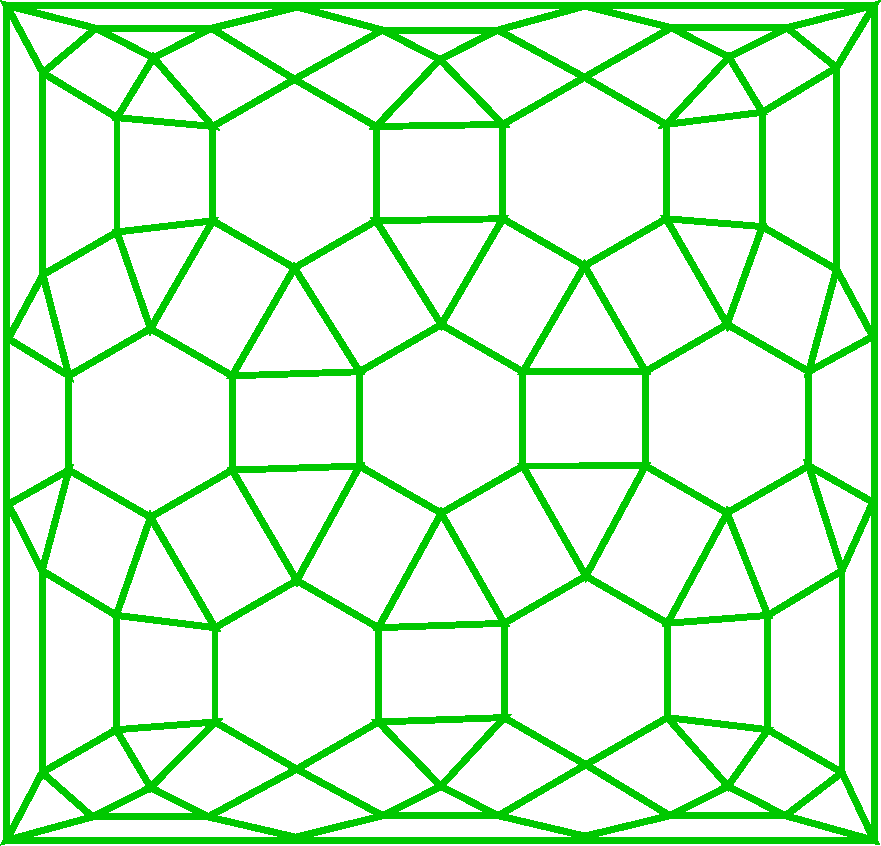
\includegraphics[scale=0.25]{infill_pattern_transformed_crop}
    \caption{\small \label{infill_pattern_transformed}}
  \end{subfigure}
%\hspace*{0.15in}
  \vspace*{0.05in}
  \begin{subfigure}[t]{1.7in}
    %\centering
    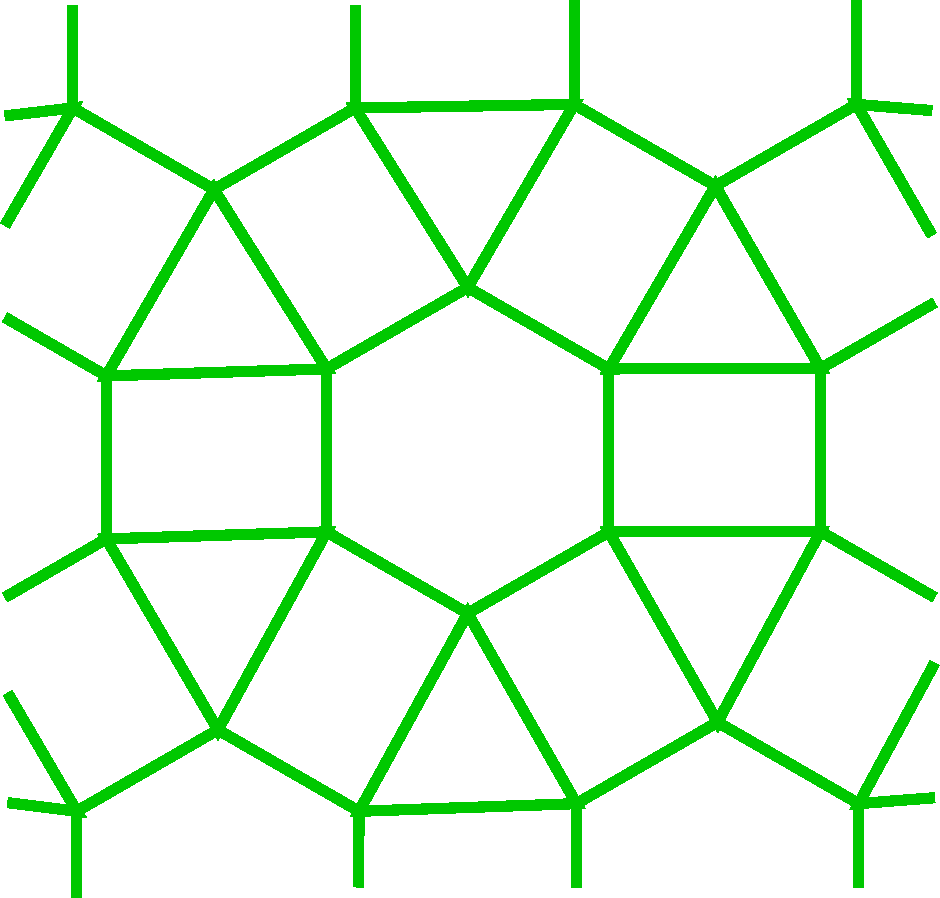
\includegraphics[scale=0.25]{infill_pattern_transformed_polygon_cut_crop}
    \caption{\small \label{infill_pattern_transformed_polygon_cut}}
  \end{subfigure}
%\hspace*{0.15in}
  \begin{subfigure}[t]{1.7in}
    %\centering
    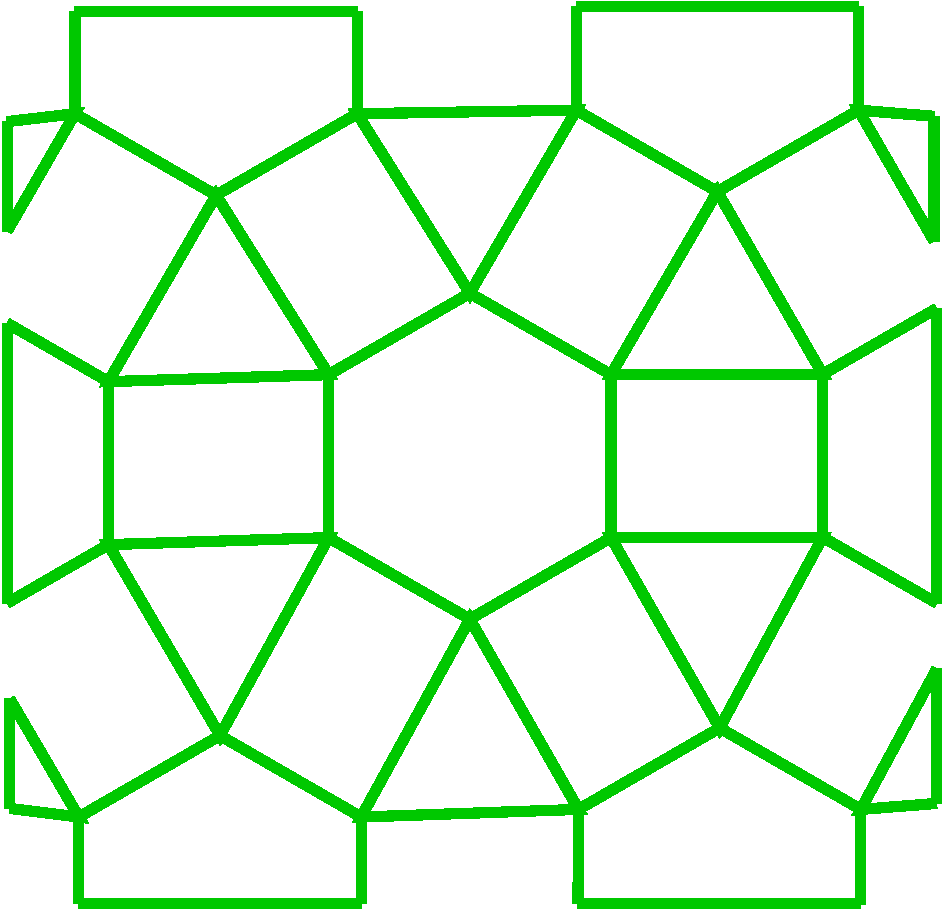
\includegraphics[scale=0.25]{infill_pattern_transformed_polygon_cut_patch_simple_crop}
    \caption{\small \label{infill_pattern_transformed_polygon_patch_simple}}
  \end{subfigure}
  %\vspace*{0.05in}
  %\hspace*{-0.1in}
  \begin{subfigure}[t]{2.5in}
    %\centering
    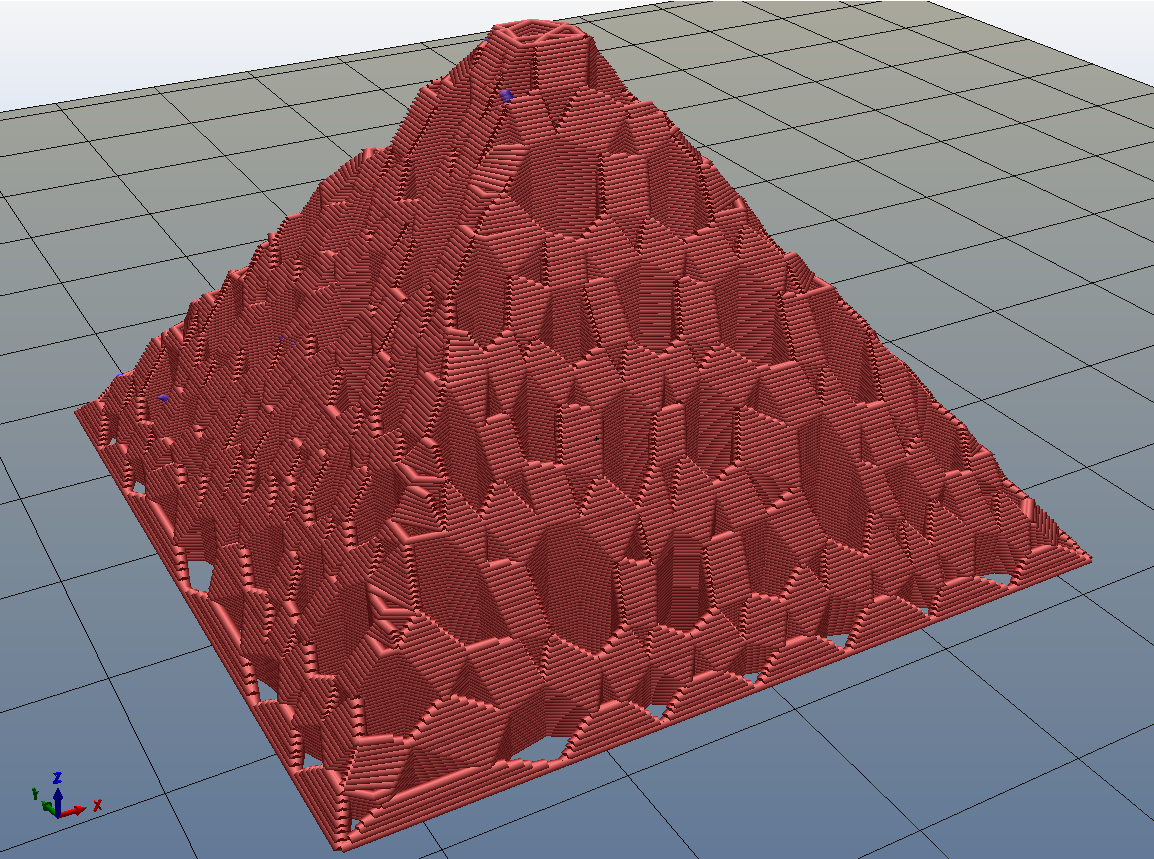
\includegraphics[scale=0.15, bb=0 0 1154 859]{PyramidPlan} 
    \caption{\small \label{pyramidplan}}
  \end{subfigure}
%\hspace*{0.15in}
  \begin{subfigure}[t]{2.5in}
    %\centering
    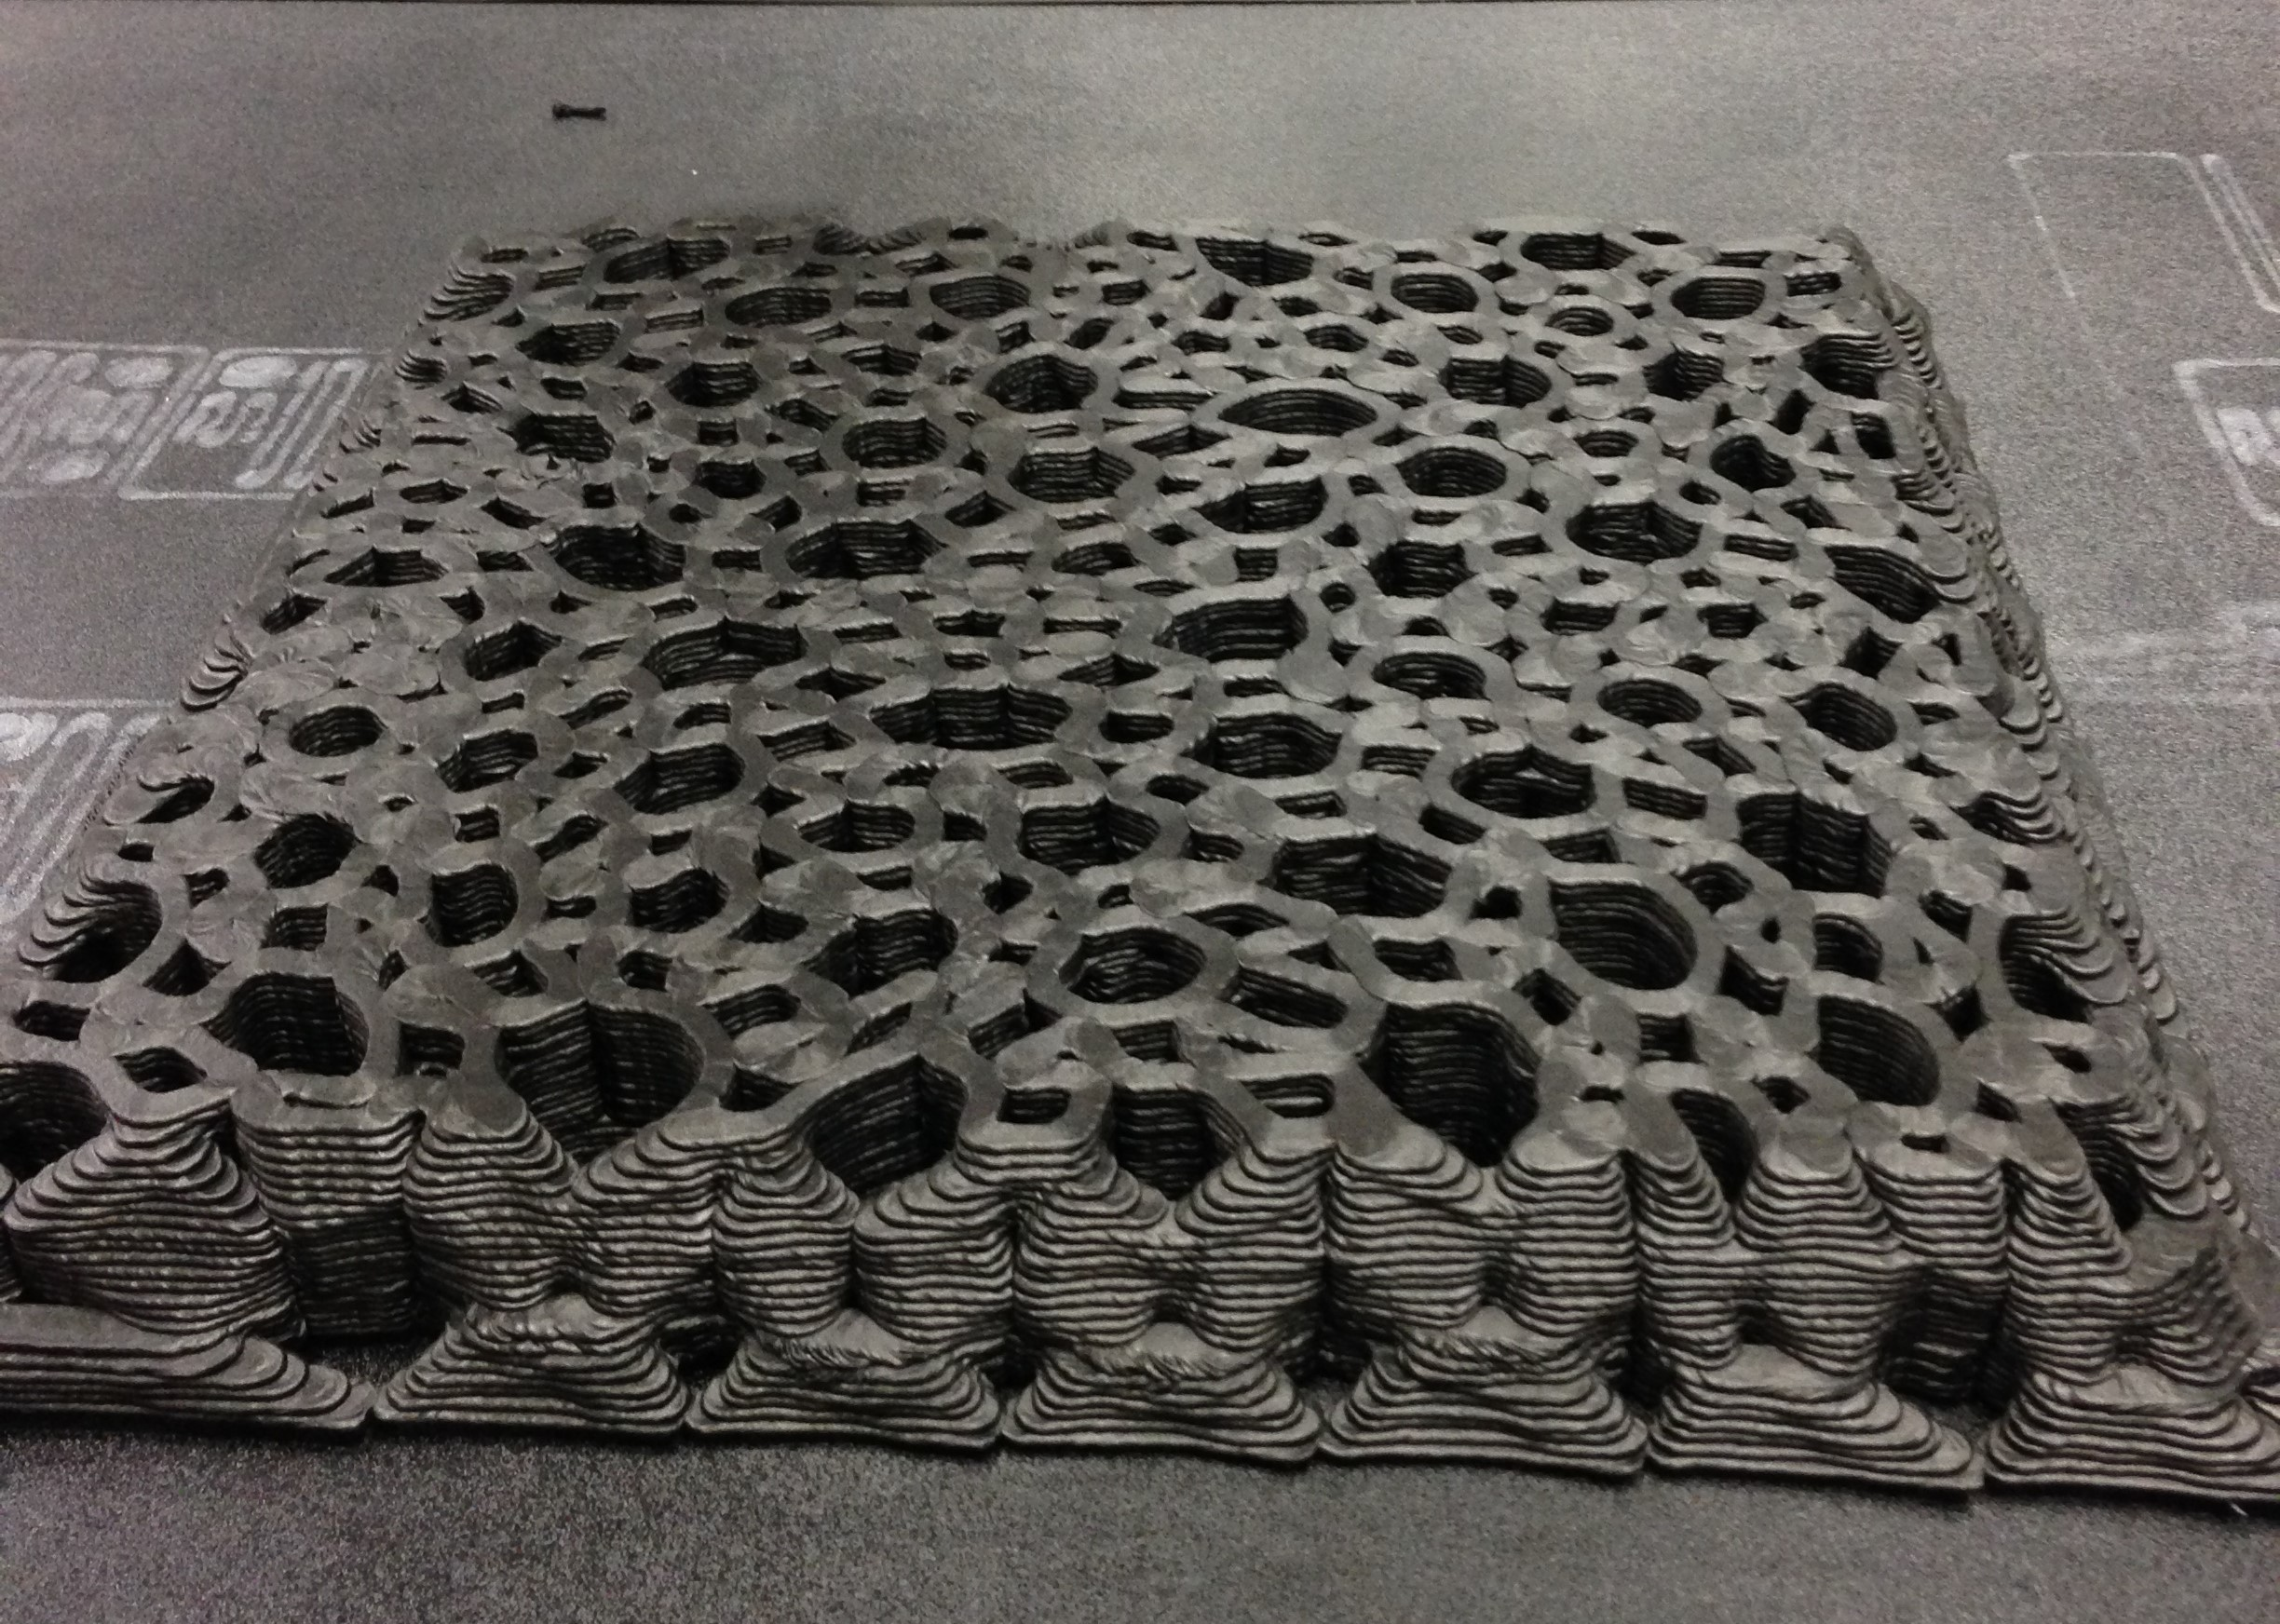
\includegraphics[scale=0.075, bb=0 0 2448 1744]{PrintedPyramid}
    \caption{\small \label{printedpyramid}}
  \end{subfigure}
  %\vspace*{-0.1in}
  \caption{ \label{infill_pattern_work_flow}
    Illustration of our framework (see Section \ref{ssec:contrib} for details).
    Subfigures (g: plan) and (h: mid-print slice) show an implementation for a  $610\,$mm $\times$ $610\,$mm $\times$ $610\,$mm pyramid.
    We plan to present complete details of our implementation in a separate manuscript.
    %\vspace*{-0.1in}
  }
\end{figure}

\subsection{Related work}

%\input{Journal_prior_ET2d}

%\input{SCF_backg3d}
%\subsection{Euler Graph} \label{sec:previouseulerwork}
\paragraph{Euler Graph.} \label{sec:previouseulerwork}
The $1$-skeleton of $K$ is an undirected planar graph ($G$).
One approach to make $G$ Eulerian is to delete a minimal number of vertices and/or edges.
But Cai and Yang~\cite{CaYa2011} showed that the Euler vertex deletion and Euler edge deletion problems are NP-Complete.
More importantly, removing edges and/or vertices could create gaps in the coverage of the domain, potentially affecting the mechanical properties of the final product.
Another approach to make $G$ Eulerian is to add a minimum number of edges that pair odd degree vertices in $G$, which can be cast as a \emph{graph augmentation} problem.
Boesch~\cite{TCR1977} presented a polynomial time algorithm for this problem, but planarity of $G$, which is necessary to avoid material collision, is not guaranteed after the augmentation.
Another approach for augmentation is to use the Chinese postman problem to double the edges along shortest paths connecting odd degree vertices in $G$.
But printing the resulting multigraph could be challenging due to non-uniform thickness of (multiple copies of) edges and non-uniform degrees of nodes.
In fact, the degree of some of the nodes could be multiplied by up to $n^o/2$, where $n^o$ is the number of odd degree vertices in $G$.
Visiting a vertex a large number of times could reduce quality of the print.

Jin et al.~\cite{JiHeFuZhDu2017} showed that subpaths in this setting could be generated using a geometric approach and then joined optimally to reduce the amount of jumps.
And Zhao et al.~\cite{ZhGuHuGaYoChBeZhCoDaBa2016} proposed a method that can find global continuous paths using Fermat spirals.
But both of these approaches are designed for completely filling the region (with or without holes), and not for sparse infilling.
   
The Catmull-Clark subdivision \cite{CatmullClark1978} creates quadrilateral polygons from any input $2$-complex.
But some vertices in the resulting mesh may have odd degrees.
% it may produce Hence may have some vertices with odd degree or even degree with at least degree $6$. Odd degree vertices creates discontinuous print path in case every edge in $1$-skeleton of the complex must be printed.
%Analogous to Catmull-clark subdivision scheme Bajaj el at \cite{ChJoGu2001} developed a hexahedral $3$-cell $3$-complex for any arbitrary $3$-complex, where vertices in $3$-cell has degree $3$. Similarly there may be some extraordinary vertices with odd degree.

Our Euler transformation appears similar to the Doo-Sabin subdivision \cite{DoSa1978},
%But Doo-Sabin could produce odd degree vertices on the boundary of the domain, the underlying space is not preserved, and copies of cells retained from the original complex may not preserve interior angles.
%Further, positions of new vertices in the Doo-Sabin subdivision are strictly prescribed, making it hard to control quality of the mesh.
%Finally, combinatorial changes of cells retained from the input complex are not permitted in this subdivision.  
%The Doo-Sabin subdivision
which creates new vertices for each polygon after $k+1$ iterations specified as
\[v_i^{k+1} = \sum_{j =1}^{n} a_{ij} v_j^{k}, ~~\mbox{ where }\]
\[a_{ii} = \frac{n + 5}{4n} ~\mbox{ and }\] 
\[a_{ij} = \frac{3 + 2 \cos(2\pi\frac{(i -j)}{n})} {4n}, \] 
where $n$ is number of vertices of the polygon and $\sum_{j=1}^{n}a_{ij} = 1$.
We outline key differences between the Doo-Sabin and our Euler transformation below.    
\begin{itemize}
  \item
    Doo-Sabin subdivision does not preserve the underlying space, and creates boundary vertices with odd degree, as shown in Figure \ref{fig:exampdooeulercombinat}.
    It will add $O(b)$ jumps, where $b$ is the number of boundary vertices after subdivision.%\add{What are the units of this retraction?}   
  \item
    New vertices are created in the Doo-Sabin subdivision based on vertices and the number of edges in the original polygon.
    But in our Euler transformation, new vertices are created through mitered offsets (parallel offset of neighboring edges) of polygons as shown in the Figure \ref{fig:exampdooeulercombinat}.
    Suppose $e_{ij}^1$ is an edge created in a polygon after the first iteration of Doo-Sabin.
    %Then we have that
    %\[\norm{e_{ij}^1} =  \frac{n + 5}{4n}\norm{e_{ij}^0} = (0.25 + \frac{1.25}{n})\norm{e_{ij}^0}.\]
    %This setting implies that $0.25 \norm{e_{ij}^0} < \norm{e_{ij}^1} < 0.67\norm{e_{ij}^0}$ as $n \geq 3$.
    For large values of $n$, we get that $\norm{e_{ij}^1} \approx 0.25 \norm{e_{ij}^0}$, whereas in our Euler transformation, the edge lengths are flexible as they depend on the mitered offsets chosen rather than on $n$. 

  \item Original angles are not preserved in the Doo-Sabin subdivision, as illustrated in Figure \ref{fig:exampdooeulercombinat}. 

  \item Combinatorial changes are not allowed in the Doo-Sabin subdivision, where as our Euler transformation allows combinatorial changes as shown in Figure \ref{fig:exampdooeulercombinat}.
  Combinatorial changes help in avoiding extremely small edges after transformation (see Section \ref{sec:eulertransformwithcombin}). 

  \item Topological changes are not allowed in the Doo-Sabin subdivision for any concave polygon, whereas our Euler transformation allows topological changes as shown in Figure \ref{fig:exampdooeulertopochang}.
  Since new  vertices are created as convex combinations of original vertices of the input polygon in Doo-Sabin subdivision, the resulting polygon is convex.
  But it will not necessarily be contained in the original polygon.
  Details on topological changes in our Euler transformation is mentioned in Section \ref{sec:eulertransformwithTopolog}.      
\end{itemize}


\begin{figure}[ht!] 
	\centering
	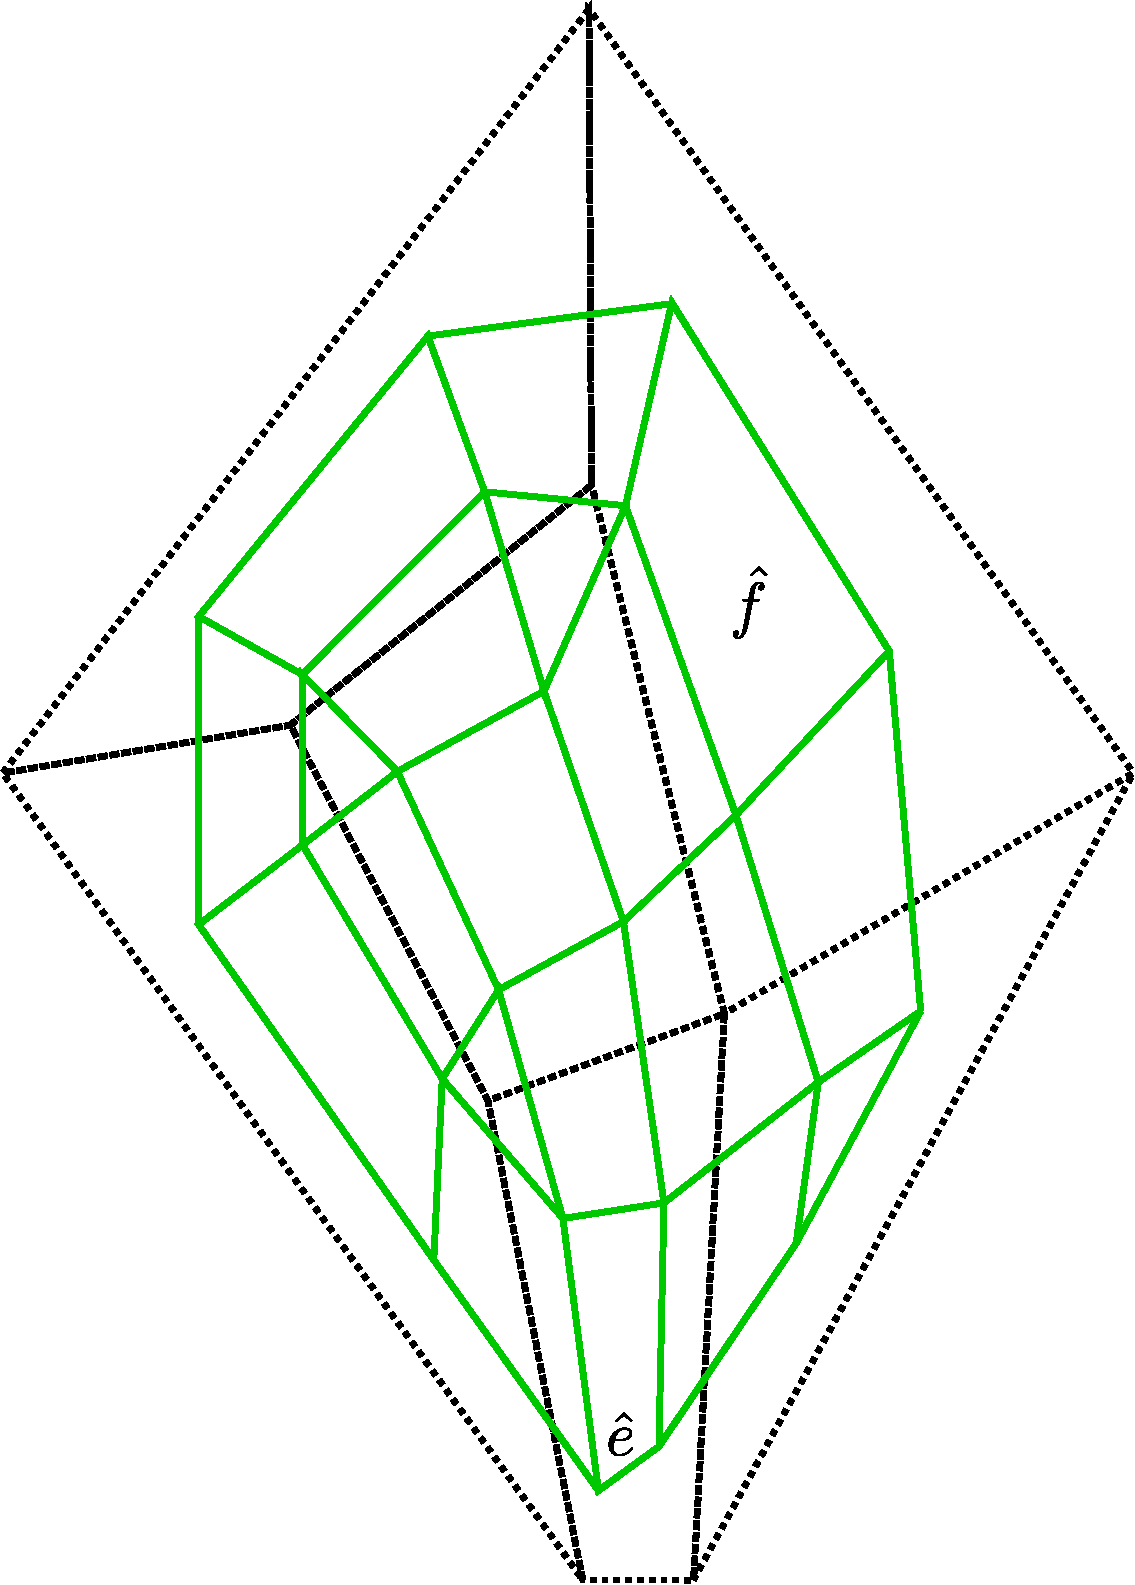
\includegraphics[scale=0.22]{doo_sabin_subdivision_example_1_crop}
	\quad
	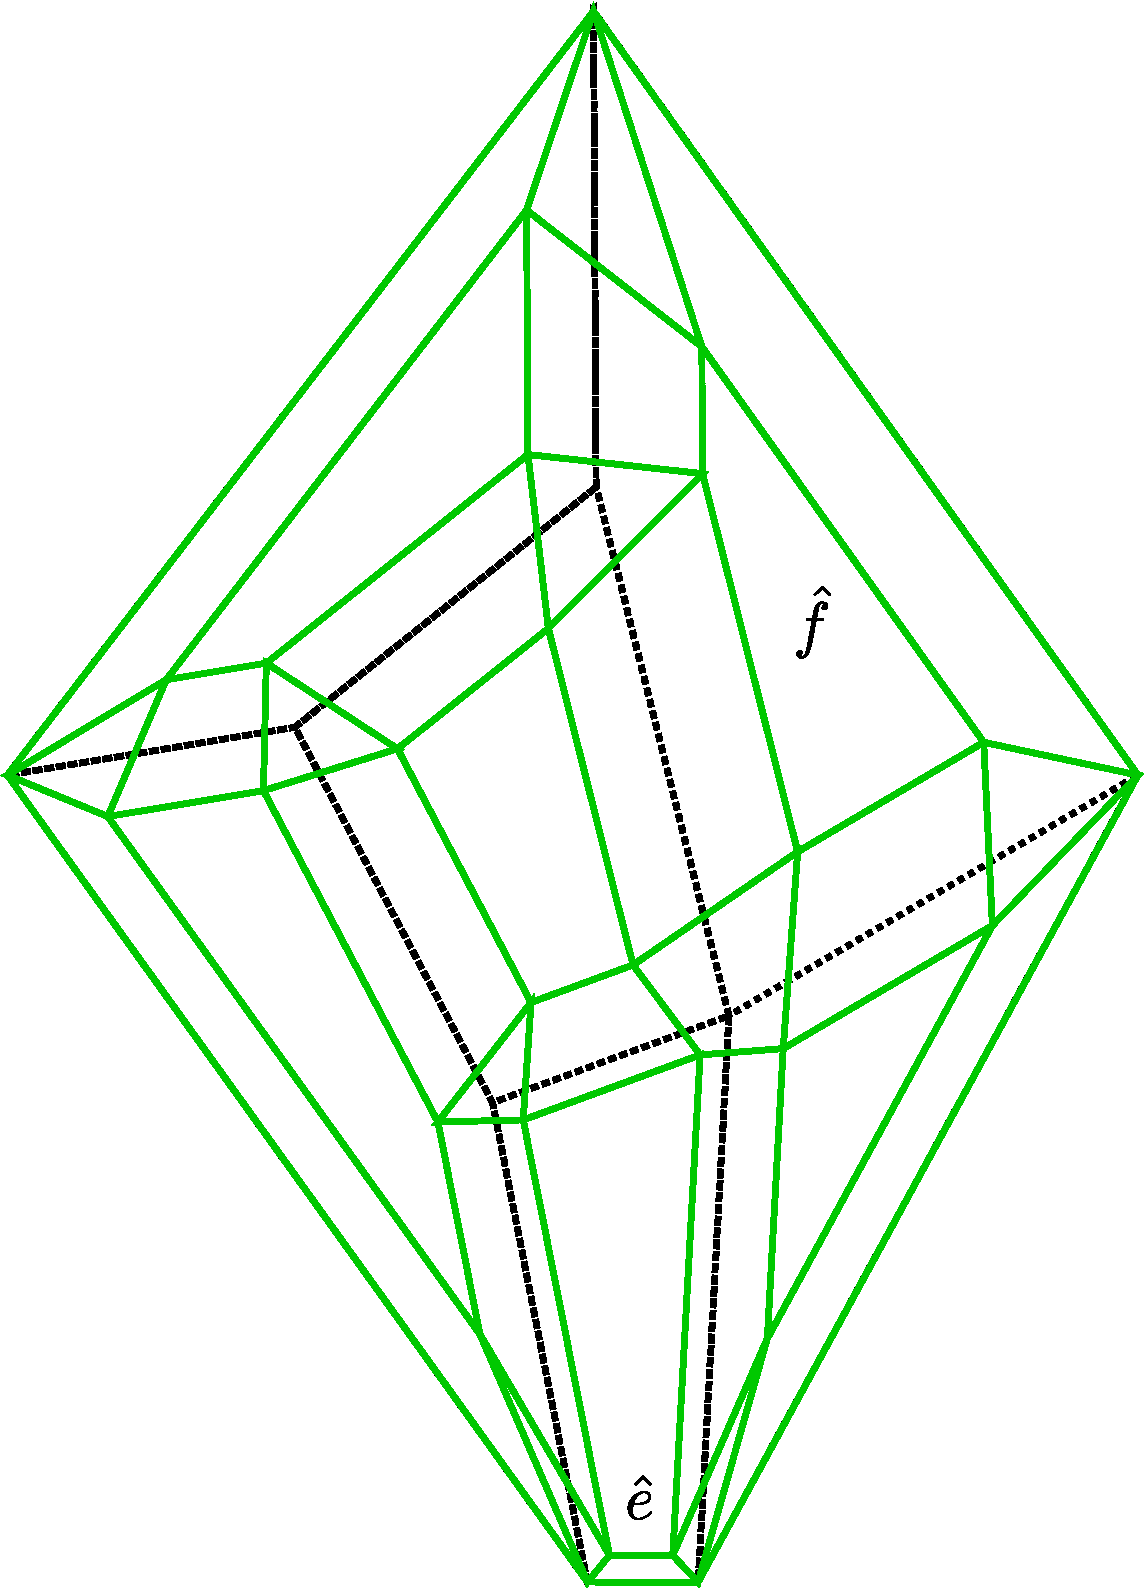
\includegraphics[scale=0.22]{euler_transformation_example_1_crop}
	\quad
	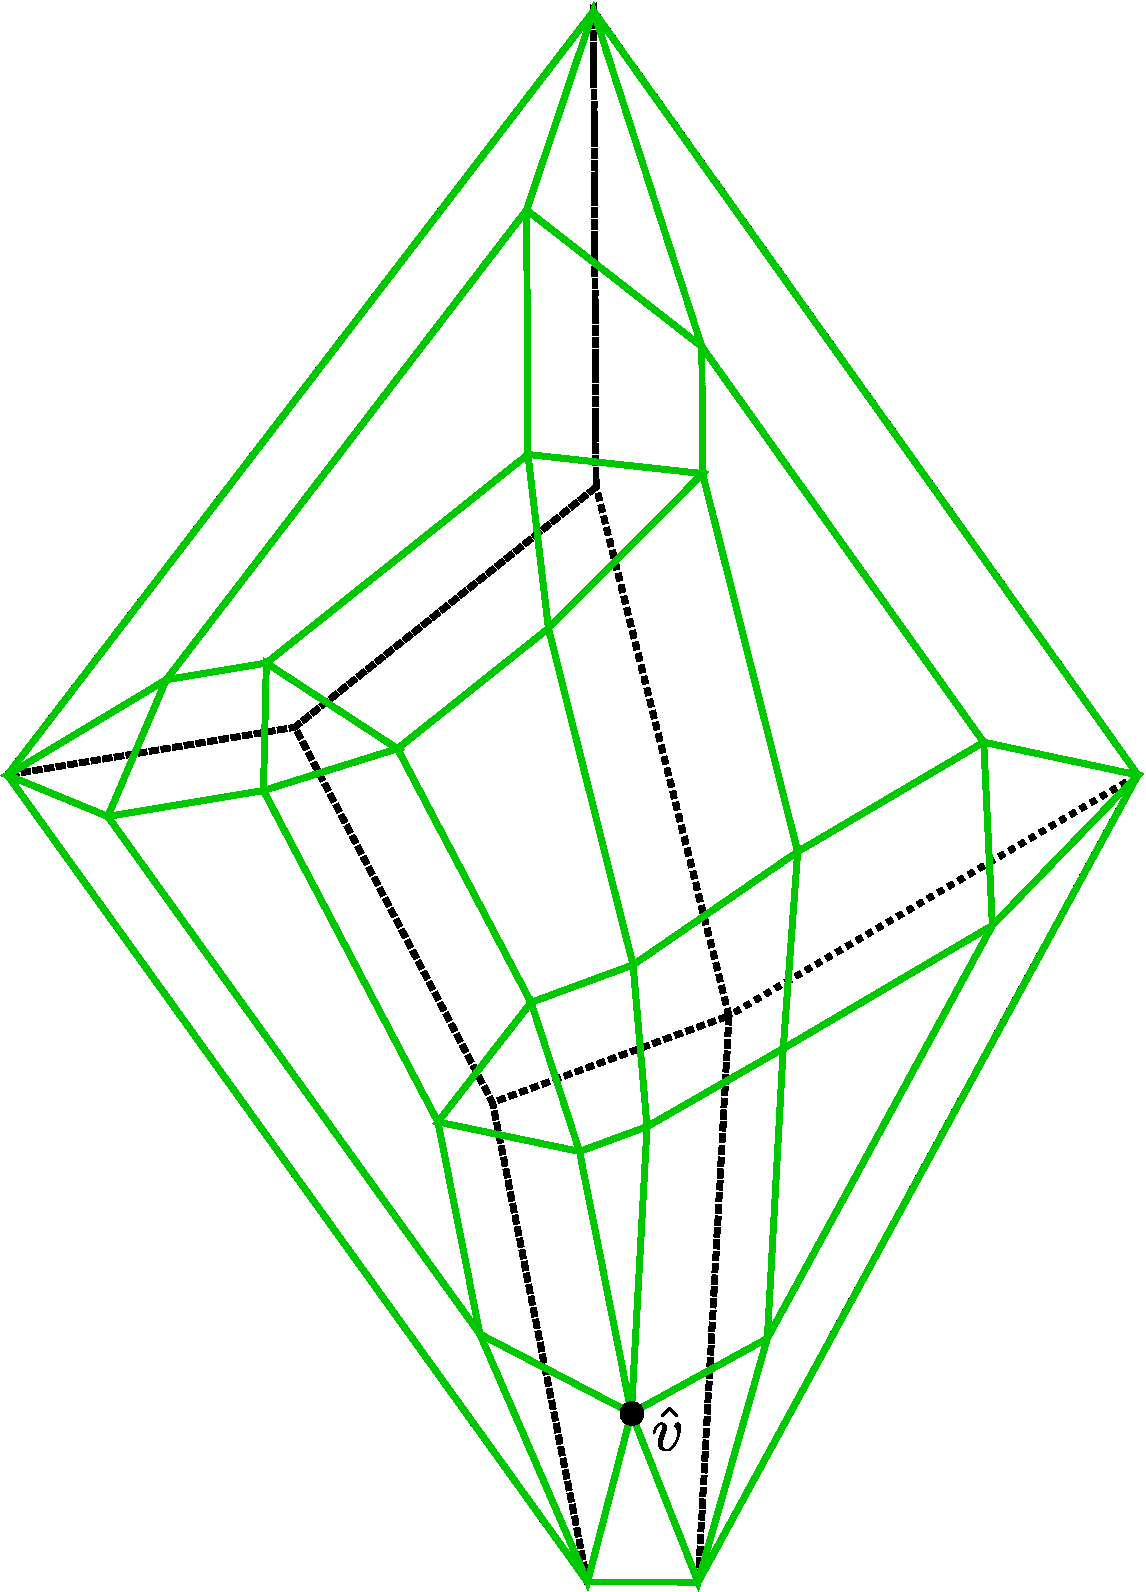
\includegraphics[scale=0.22]{euler_transformation_example_1_combinatorial_changes_crop}
	\caption{\label{fig:exampdooeulercombinat}
        Input complex $K$ (in dotted black) and three different output complexes $\hat{K}$ (in green).
        Doo-Sabin subdivision of $K$ (left), Euler transformation of $K$ without combinatorial changes (middle), and Euler transformation of $K$ with combinatorial changes (right).
        Cell $\hat{f}$ of $\hat{K}$ does not preserve the angles of input complex in the left Figure, but $\hat{f}$ of $\hat{K}$ does preserve the angles in the middle and right Figures. }
\end{figure}

\begin{figure}[ht!] 
	\centering
	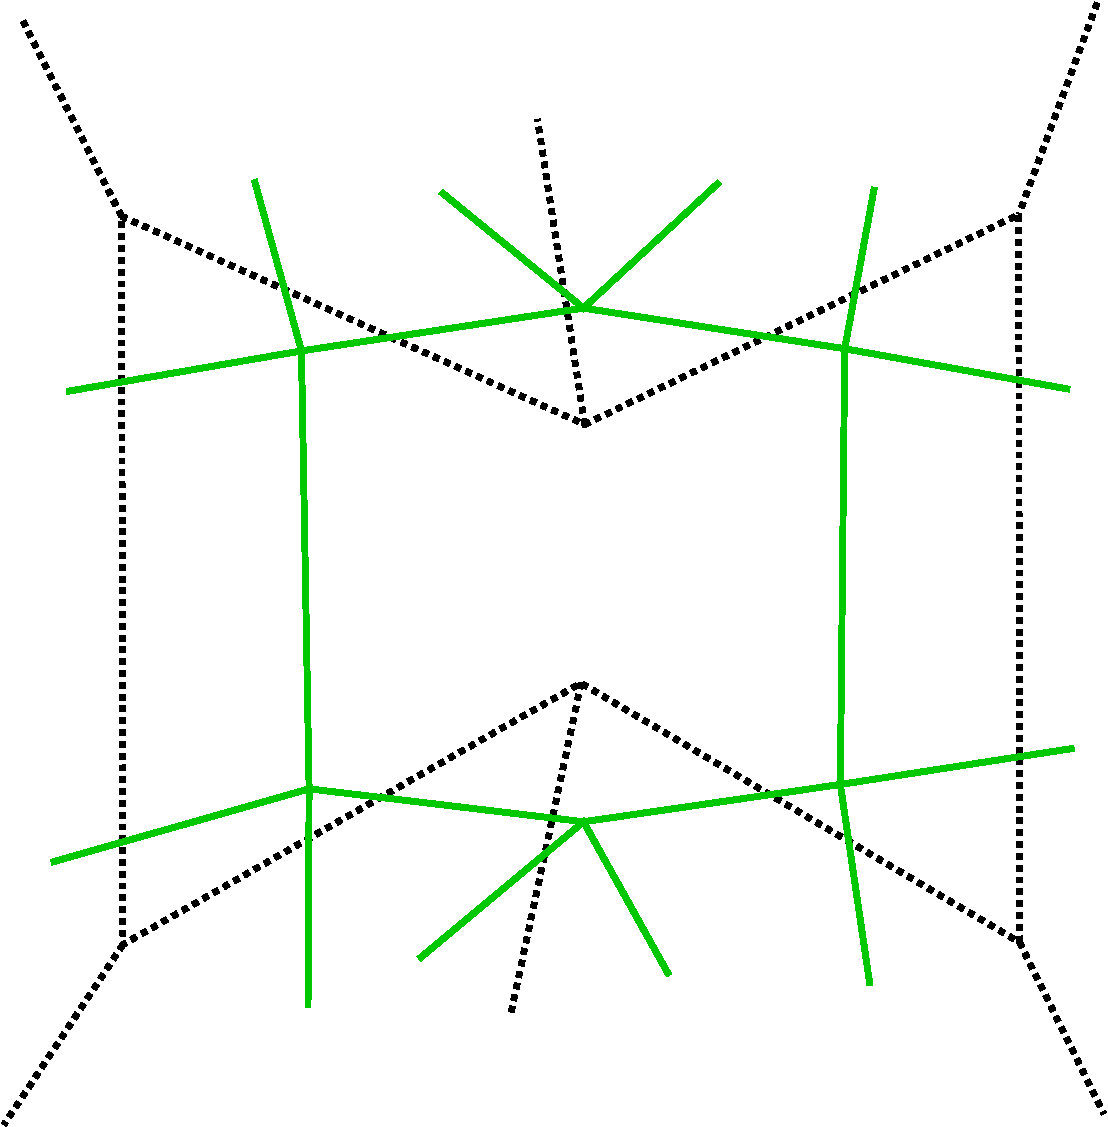
\includegraphics[scale=0.25]{doo_sabin_subdivision_example_2_crop}
	\quad
	\quad
	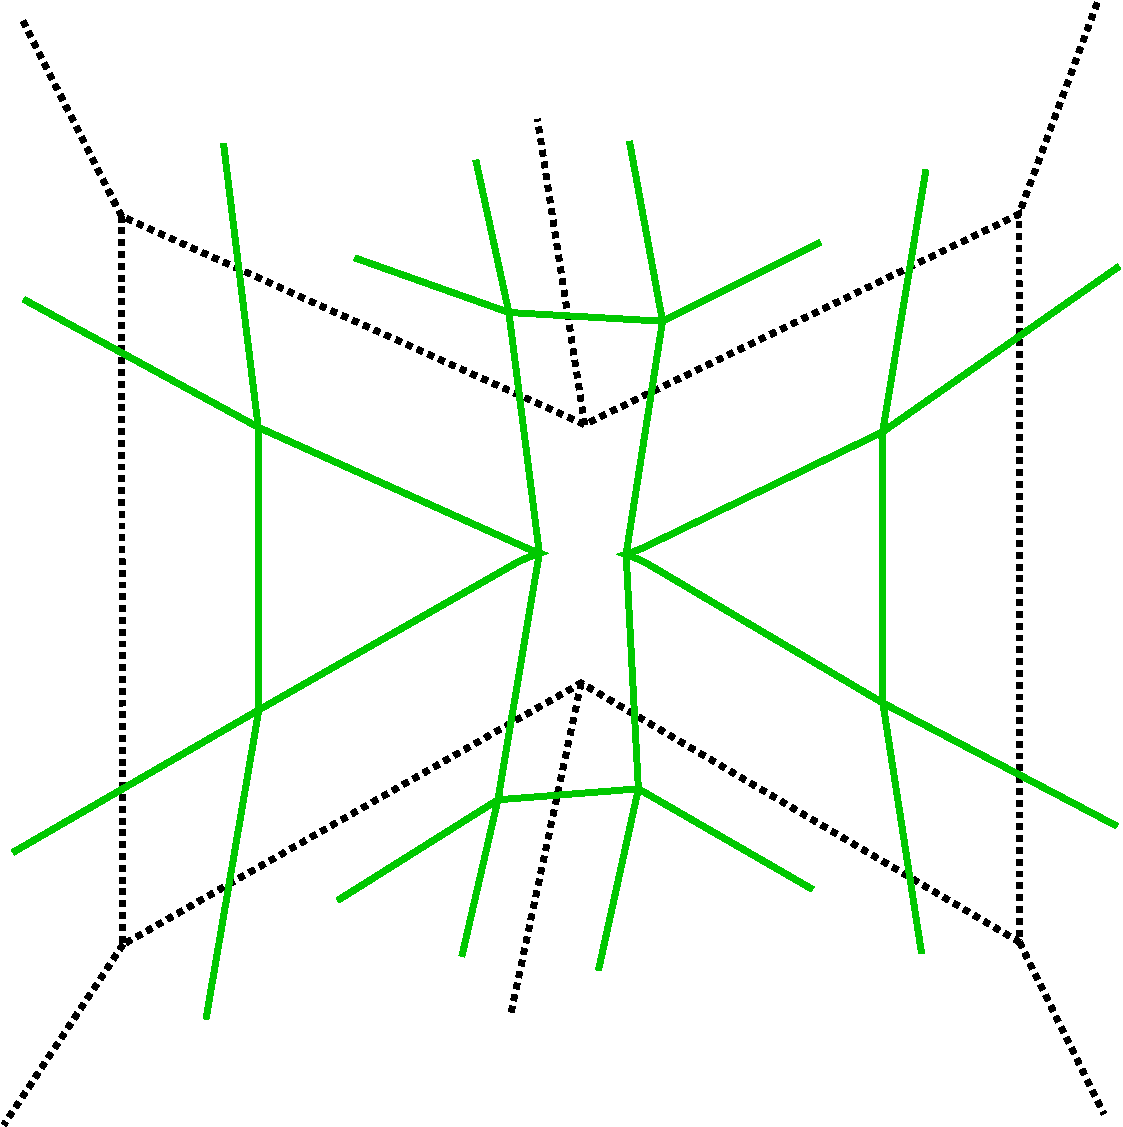
\includegraphics[scale=0.25]{euler_transformation_example_2_topological_changes_crop}
	\caption{\label{fig:exampdooeulertopochang} Doo-Sabin subdivision of a concave polygon (in dotted black) in input complex $K$ (left) and the Euler transformation of the same polygon with topological changes only (right).
        }
\end{figure}


%Our undirected graph($1$-skeleton of $\hat{K}$) is symmetric. Since graph is both edge transitive and vertex transitive implies symmetry. It is also $4$-regular, since every symmetric graph is regular. If we allow combinatorial changes then some of the vertices will have degree $6$ due to local Euler transformation. Hence even in worst case any vertex will be visited at most $3$ times.


\paragraph{Tool path}\label{sssec:toolpath}

While the perimeter and inset can typically be printed as continuous loops, tool path planning for printing the infill lattice commonly generates tool paths resembling a back and forth pattern, a spiral, or a fractal-like path for an arbitrary geometry.
The tool path consists of \textit{print paths} (material is pushed through the nozzle) and \textit{travel paths} (extruder moves from one location to other without pushing material).
Galceran and Carreras \cite{GaCa2013} described coverage path planning as assignment of finding a path that passes through all the points without obstacles.
Xu \cite{Xu2011} presented the use of graph-based algorithms in coverage problems.
General requirements for graph-based coverage problems such as all vertex coverage, non-overlapping and continuous paths, etc.~\cite{CaHuHa1988} are applicable in 3D printing as well, including the requirement that each edge should be printed.
One of the major steps in path planning is the identification of the tool path trajectory~\cite{DiPaCuLi2015}.
This tool path generation step involves filling interior regions and joining sub paths \cite{JiHeDu2017}.
While attempts have been made to join sub paths into a continuous path, they are all limited by increasing complexity of geometry.
Fewer sub paths in the tool path trajectory implies better quality of print.

Wang et al.~\cite{KuWuWa2019} developed $3$-dimensional infill (crossfill) using space filling curves, whose layer by layer cross-section is a continuous curve.
Crossfill curves are fit into the infill region by intersecting with boundary of the polygon in a given layer, but this step can create multiple components.
Later these components are connected into one continuous curve through an outer perimeter.
New edges added to create these components are not guaranteed to have a support below it.
We can still have material collision in each individual component if their boundary is too skewed or component is too thin (this is still an open problem; see Section \ref{sec:boundaryedges}). 
 
Use of graphical models in additive manufacturing was demonstrated recently by Dreifus et al.~\cite{Dretal2017}.
They mesh each layer of the print as a graph, and find an Eulerian cycle over all edges of the graph.
If the infill lattice is not Eulerian, they add "phantom edges" to the odd-degree vertices of the graph.
When the extruder reaches an odd degree vertex, it stops printing, lifts above the printed material, moves to its matched vertex, and resumes printing.
However, these stop and starts leave \textit{teardrops} of material in their wake, as the extruder drags excess material behind it.
Such teardrops weaken the print.
Also, stopping and starting repeatedly increases print times.
Further, their approach to identify the Eulerian cycle created \emph{crossovers} when pairs of sub-paths of the tour cross each other.

%\begin{comment}
%Add figures for all the defects we discussed delamination, saging, teardrop.
%\end{comment}

\section{Slicing}\label{sec:slicing}
The goal of our 3D printing approach is to have maximum continuous print path and minimum travel path (i.e., non-print path) in each layer.
Further, when printing multiple layers on top of each other, we want to ensure there is no printing in free space.
Ensuring we avoid printing in free space depends crucially on the geometric complexity of the object as well as on the first round of slicing.
We first formalize the condition that the sequence of layers generated by slicing must satisfy in order to prevent printing in free space (Section \ref{subsec:contilayers}).
We assume this condition is satisfied by the layers of the input to our \emph{clipping} procedure, which produces meshes for each polygon in a layer that are guaranteed to be Euler (Section \ref{subsec:clipping}).
 
%\input{Journal_epscont}
\subsection{$\epsilon$-Continuous Layers}\label{subsec:contilayers}
Let $\Ps_i = \{P_{ij}\}$ and $\Ps_{i+1} = \{P_{i+1,j}\}$ are sets of the polygons in two consecutive layers created by slicing.
The two layers are said to be $\epsilon$-continuous if for every point $\vx \in P_{i+1,j}$ there exists a point $\vy$ in \emph{some} $P_{ij} \in \Ps_i$ such that $ d(\vx, \vy) \leq \epsilon$ for \emph{all} $P_{i+1,j} \in \Ps_{i+1}$, where  $\epsilon = c r$ with $0 \leq c \leq 1$ and $r$ being the radius of extruder. % (see Figure \ref{fig:epsiloncontinuous}).
The parameter $c$ determines the maximum \emph{overhang} allowed for the material deposited in a layer over the material in the layer immediately below.
We assume there are sufficient numbers of perimeters in each layer to support the boundary edges in the layer above.
%Assuming the numbers of perimeters in the two layers are same, if two consecutive layers are not $\epsilon$-continuous then the print may collapse due to printing in free space.
%While one may be able to use varying numbers of perimeters in consecutive layers to avoid printing over free space in certain settings,
Value of $c$ is chosen based on various design and material considerations.
We assume the output of the slicing step in the design process produces layers that are $\epsilon$-continuous in consecutive pairs.

%\input{Journal_clip}
\subsection{Clipping}\label{subsec:clipping}
Suppose $\hK$ is the Euler transformation of $K$, which meshes the union of polygons $\displaystyle \cup_i \Ps_i = \cup_{i,j} P_{ij}$ from all layers, where $P_{ij} \in \Ps_i$ is the $j$th polygon in $i$th layer.
Each polygon $P_{ij}$ has a region $R_{ij}$ to be filled with infill lattice (note that $R_{ij} \subset P_{ij}$ can happen as some polygons may have edges along the boundary of the print domain).
Suppose $\tR_{ij}$ is the inward Minkowski offset with a ball of radius $r$, the extruder radius, of the region $R_{ij}$.
We will use $\tR_{ij}$ instead of $R_{ij}$ to generate the infill lattice for $P_{ij}$.
The reason behind this step is explained in Step \ref{itm:support} (to print the Support Perimeter).
Let polygons $R_{ij}$ and $\tR_{ij}$ be represented by the clockwise-ordered sequence of vertices $\{v_1, .... , v_n\}$ and $\{\tv_1, \dots , \tv_n\}$, respectively.
We define the \emph{clip} operation for intersecting (or clipping) a $2$-complex with a polygon, which may produce a $2$-complex that may have multiple components, and may not be pure.
We also define the \emph{patch} operation that converts the $2$-complex produced by a clip operation back into a connected pure $2$-complex.
%Let clipping $\hK$ with region $R_{ij}$ produce the $2$-complex $\tK$.
%Then $\tK$ consists of $2$-cells in $K$ interior to $R_{ij}$ and free edges formed by trimming those $2$-cells in $K$ which intersect $R_{ij}$.
%$\tK$ is not guaranteed to be a pure $2$-complex, since free edges do not belongs to any $2$-cells.
%The $1$-skeleton of $\tK$ is guaranteed to have an \textit{even} number of \textit{free edges}.
%This result follows from the handshake lemma that says an undirected graph has even number of odd-degree vertices.
%Since $\hK$ is Euler, only the vertices at the ends of free edges in $\tK$ have odd degree (of $1$ each).
%Hence there must be an even number of free edges.


\begin{defn} \label{def:clip}
  \emph{({\bfseries Clip})}
  We define how to construct $\tK$, the output of clipping the $2$-complex $\hK$ with polygon $\tR_{ij}$.
  %Anything contained in $\tR_{ij}$ is may be at the boundary or interior to $\tR_{ij}$.
  Add  to $\tK$ the polygons, edges, and vertices of $\hK$ contained in $\tR_{ij}$.
  For edges in $\hK$ cut by the boundary of $\tR_{ij}$, add to $\tK$ the portions inside $\tR_{ij}$ as new edges, and their points of intersection on the boundary of $\tR_{ij}$ as new vertices.
\end{defn}
%
Note that the result of a clip operation may not necessarily be a pure $2$-complex, and can have multiple components (see \cref{fig:multicomponent}).

\begin{defn} \label{def:patch}
  \emph{({\bfseries Patch})}
  Let $\tK$ be the output of a clip operation as specified in \cref{def:clip}.
  Suppose $S= \{\tv_{n+1}, \tv_{n+2}, .... , \tv_{n+m}\}$ is a clockwise ordered sequence of all points of intersection of $\tR_{ij}$ and the $1$-skeleton of $\hK$ with odd degrees in the $1$-skeleton of $\tK$
  (note that $m$ will be even).
  Since $\tR_{ij}$ can intersect edges in $\hK$ between or at their end point(s), vertices in $S$ can be terminal or boundary vertices in the $1$-skeleton of $\tK$.
  Join alternate pair of vertices in $S$ by a clockwise path on $\tR_{ij}$ as shown in Figure \ref{fig:printingprocess}.
  There are two possible choices of joining alternate pairs of vertices ($1$-$2$, $3$-$4,\dots$ or $2$-$3$, $4$-$5,\dots$).
  Pick the option that ensures the end vertices of components represented by subsequences of $S$ are connected by these paths to end vertices of adjacent components.
  Also add new polygons to $\tK$ whose edges include the edges in new paths added as described above, new edges added by the clip operation on $\hK$, and the edges of $\hK$ contained in $\tR_{ij}$.	
\end{defn}

We show that the patch operation restores the Euler and connected nature of the input complex.

\begin{lem}\label{lem:singlecomponent}
  If $\hK$ is a connected pure $2$-complex and its $1$-skeleton is Euler, then $\tK$ produced by the patch operation on $\hK$ is a connected pure $2$-complex and its $1$-skeleton is Euler. 
\end{lem}
\begin{proof}
  Clipping $\hK$ with region $\tR_{ij}$ can create multiple components in the infill lattice if $\tR_{ij}$ intersects any polygon in $\hK$ more than two times, or an edge more than once, or all edges connected to a vertex (see \cref{fig:multicomponent}).
  Each component created in this process has an even number of odd degree vertices (by handshake lemma).

  Let $S' =\{\tv_1, \dots, \tv_p\}$ be a clockwise ordered subsequence of vertices in $S$ of some component (with $p < m$).
  As specified in \cref{def:patch}, we join alternate pairs of vertices in $S'$ by a path on $R_{ij}$ (also see the Clipping Step \ref{itm:patch}) such that edge $\{\tv_1, \tv_2\}$ is not included.
  Since $p$ is even, edge $\{\tv_{p-1}, \tv_{p}\}$ is also not included.
  Hence the first and last vertices in $S'$ ($\tv_1$ and $\tv_p$) are left unpaired, but all intermediate vertices are now connected to $\tK$.
  In this case, the patch operations (in the Clipping step) will necessarily pair $\tv_1$ with a similar unpaired end vertex of the previous component, and also pair $\tv_p$ with the unpaired start vertex of the next component.
  Hence the extra edges added by the patch steps ensure that we get a single connected component.
  Also note that each odd degree vertex gets one additional edge, thus making its degree even.
  Hence the $1$-skeleton of $\tK$ is Euler.
  Finally, the new polygons added to $\tK$ (as specified at the end of \cref{def:patch}) ensure that the resulting complex is pure.
\end{proof}
\vspace*{-0.15in}

\begin{figure}[ht!]
  \centering
  \begin{subfigure}[t]{2in}
    \centering
    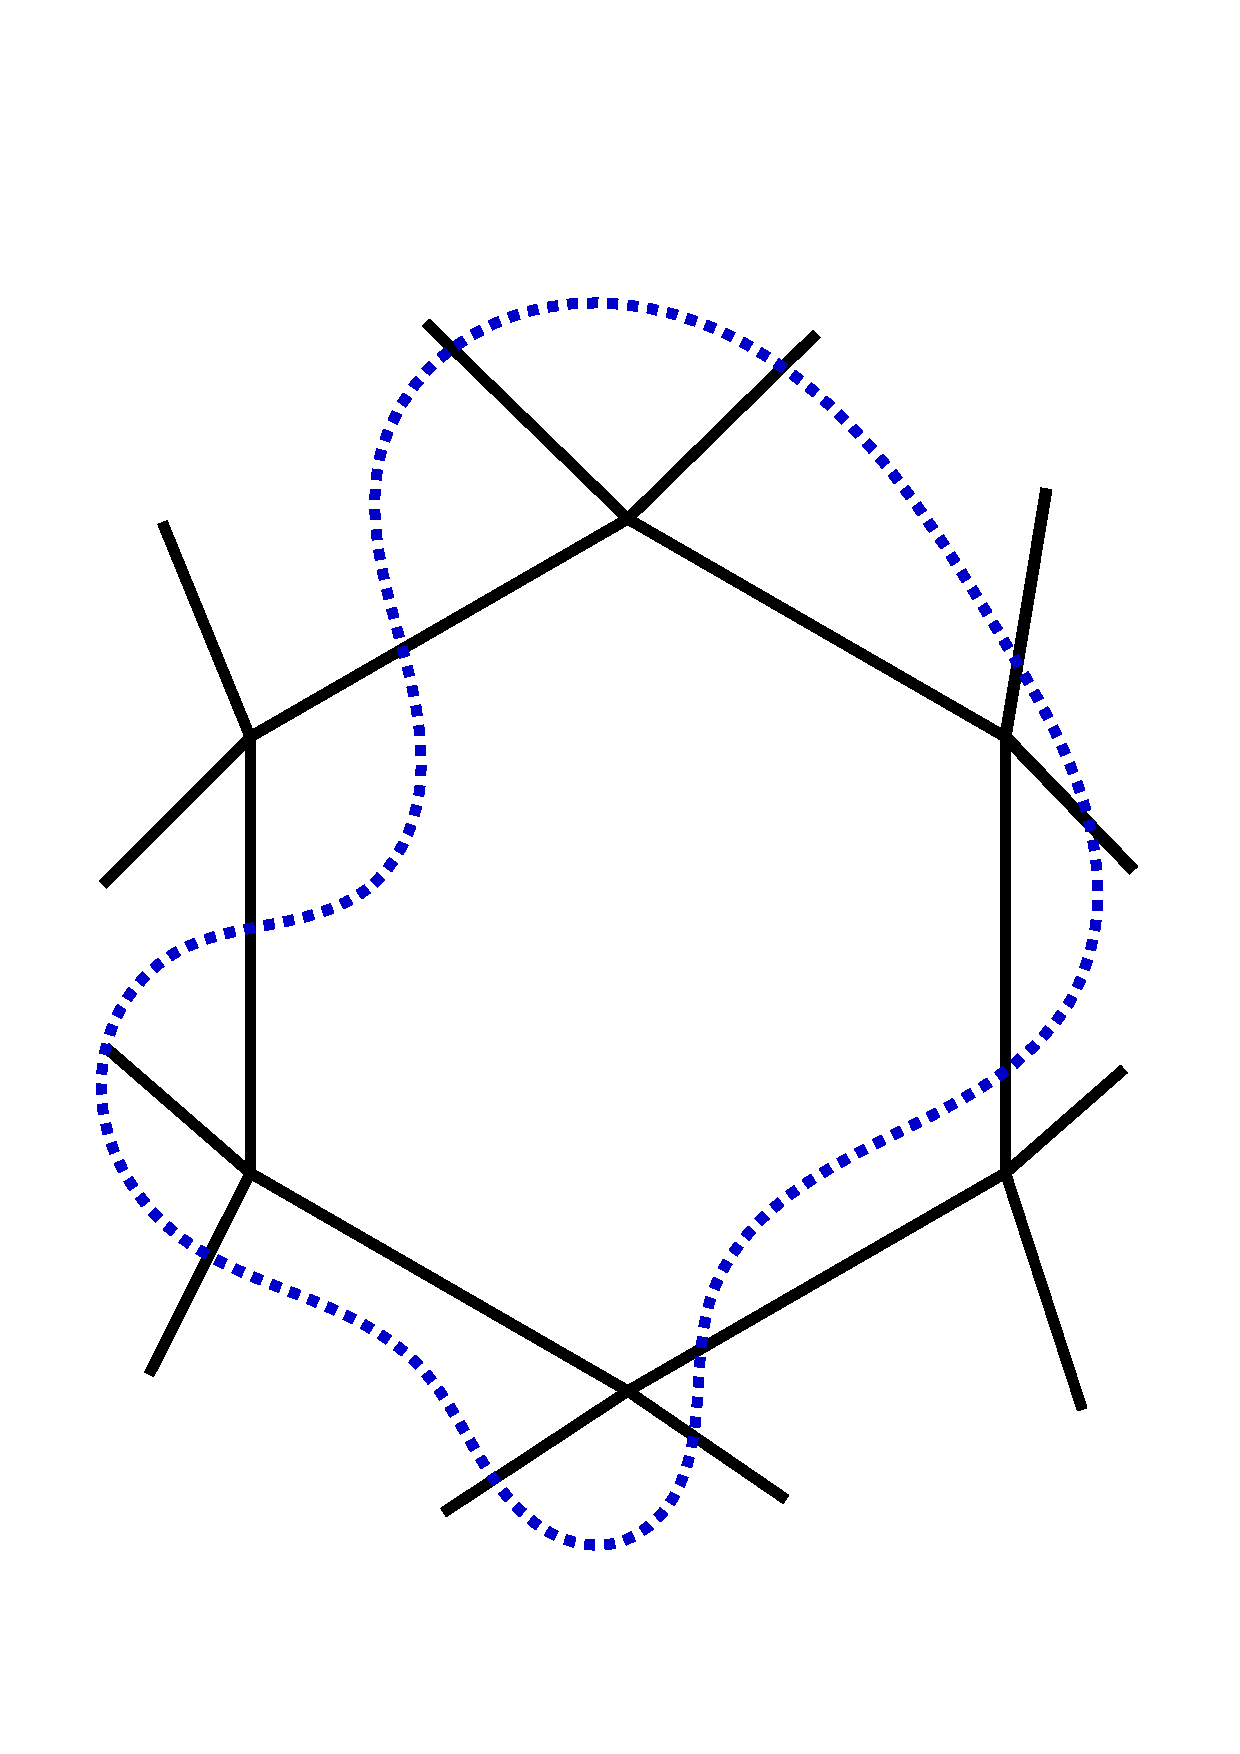
\includegraphics[scale=0.20]{multi_component_fig_1_crop}
    \caption{\label{fig:multicomponenta}}
  \end{subfigure}
  \begin{subfigure}[t]{2in}
    \centering
    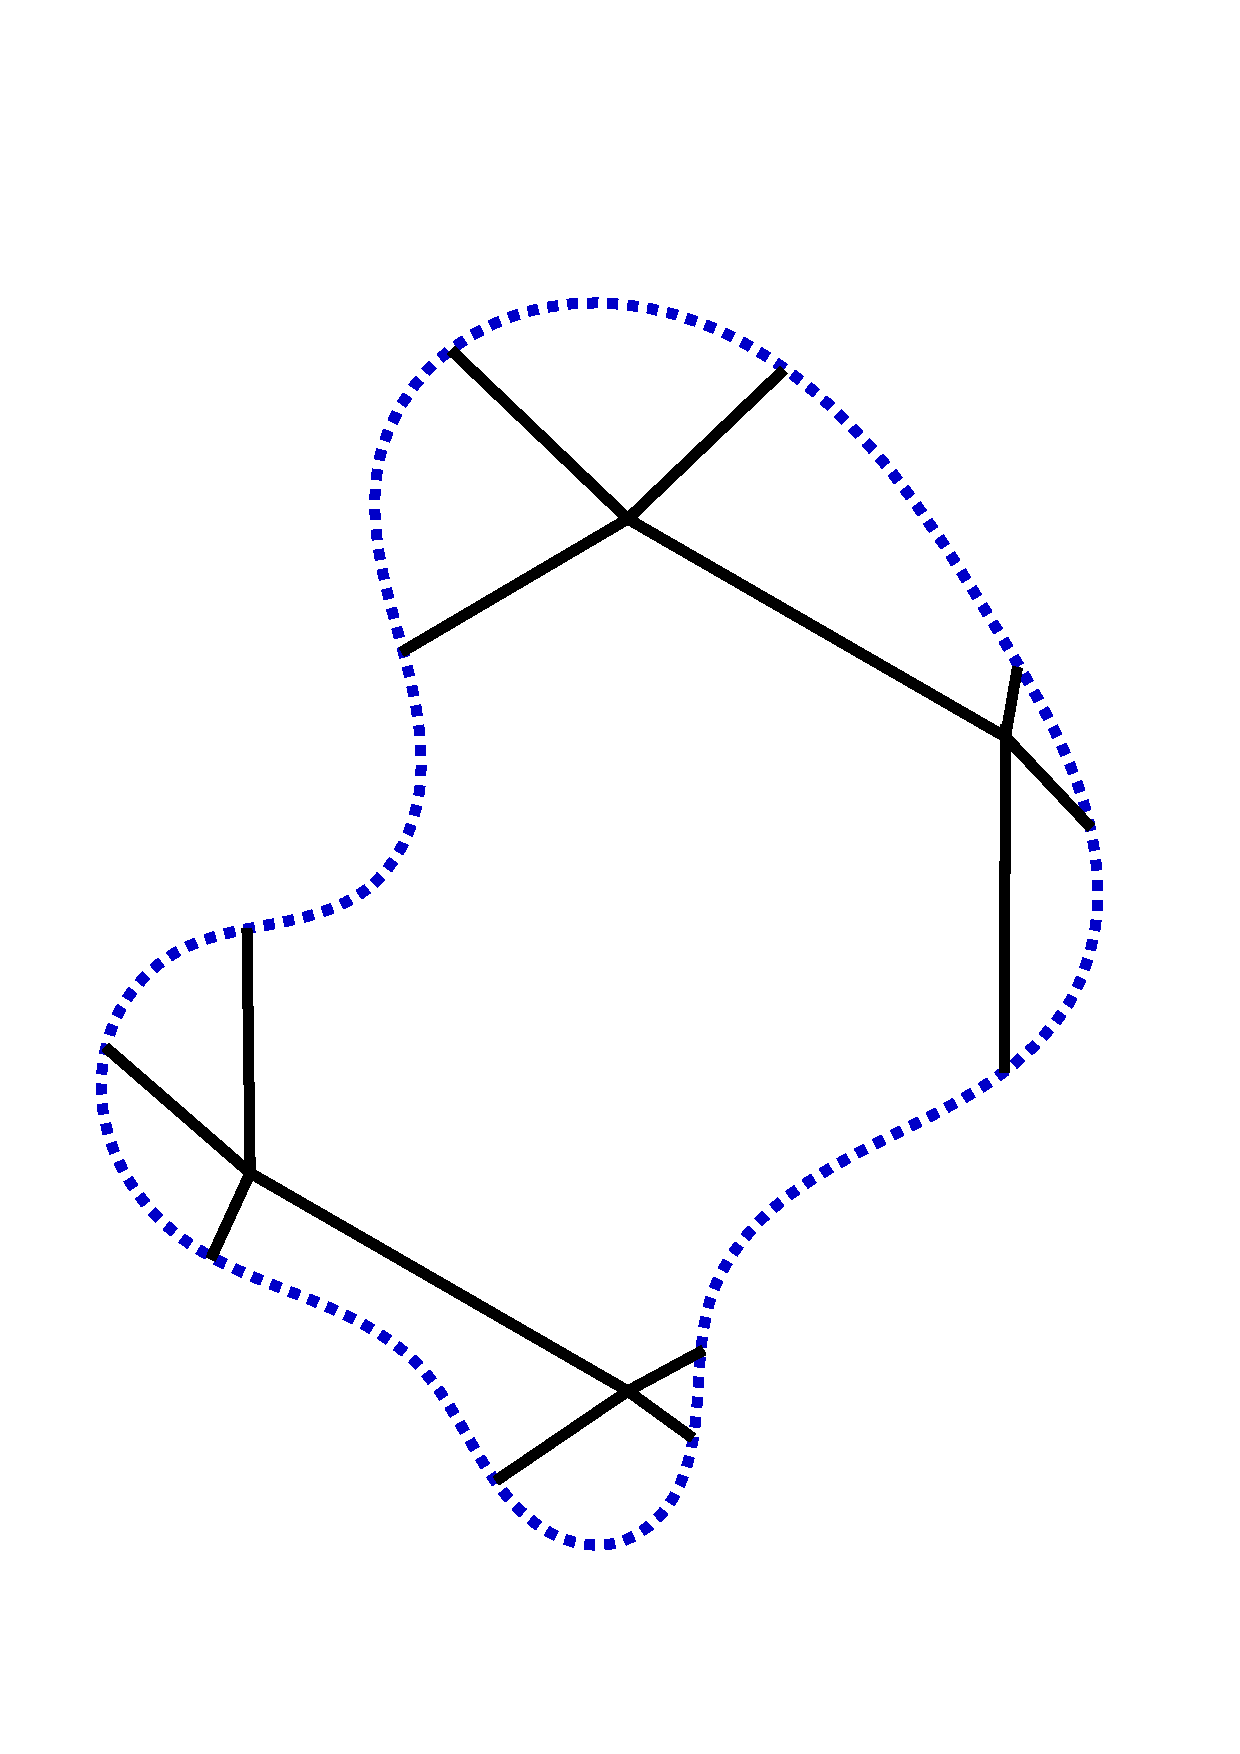
\includegraphics[scale=0.20]{multi_component_fig_2_crop}
    \caption{\label{fig:multicomponentb}}
  \end{subfigure}
  \begin{subfigure}[t]{2in}
    \centering
    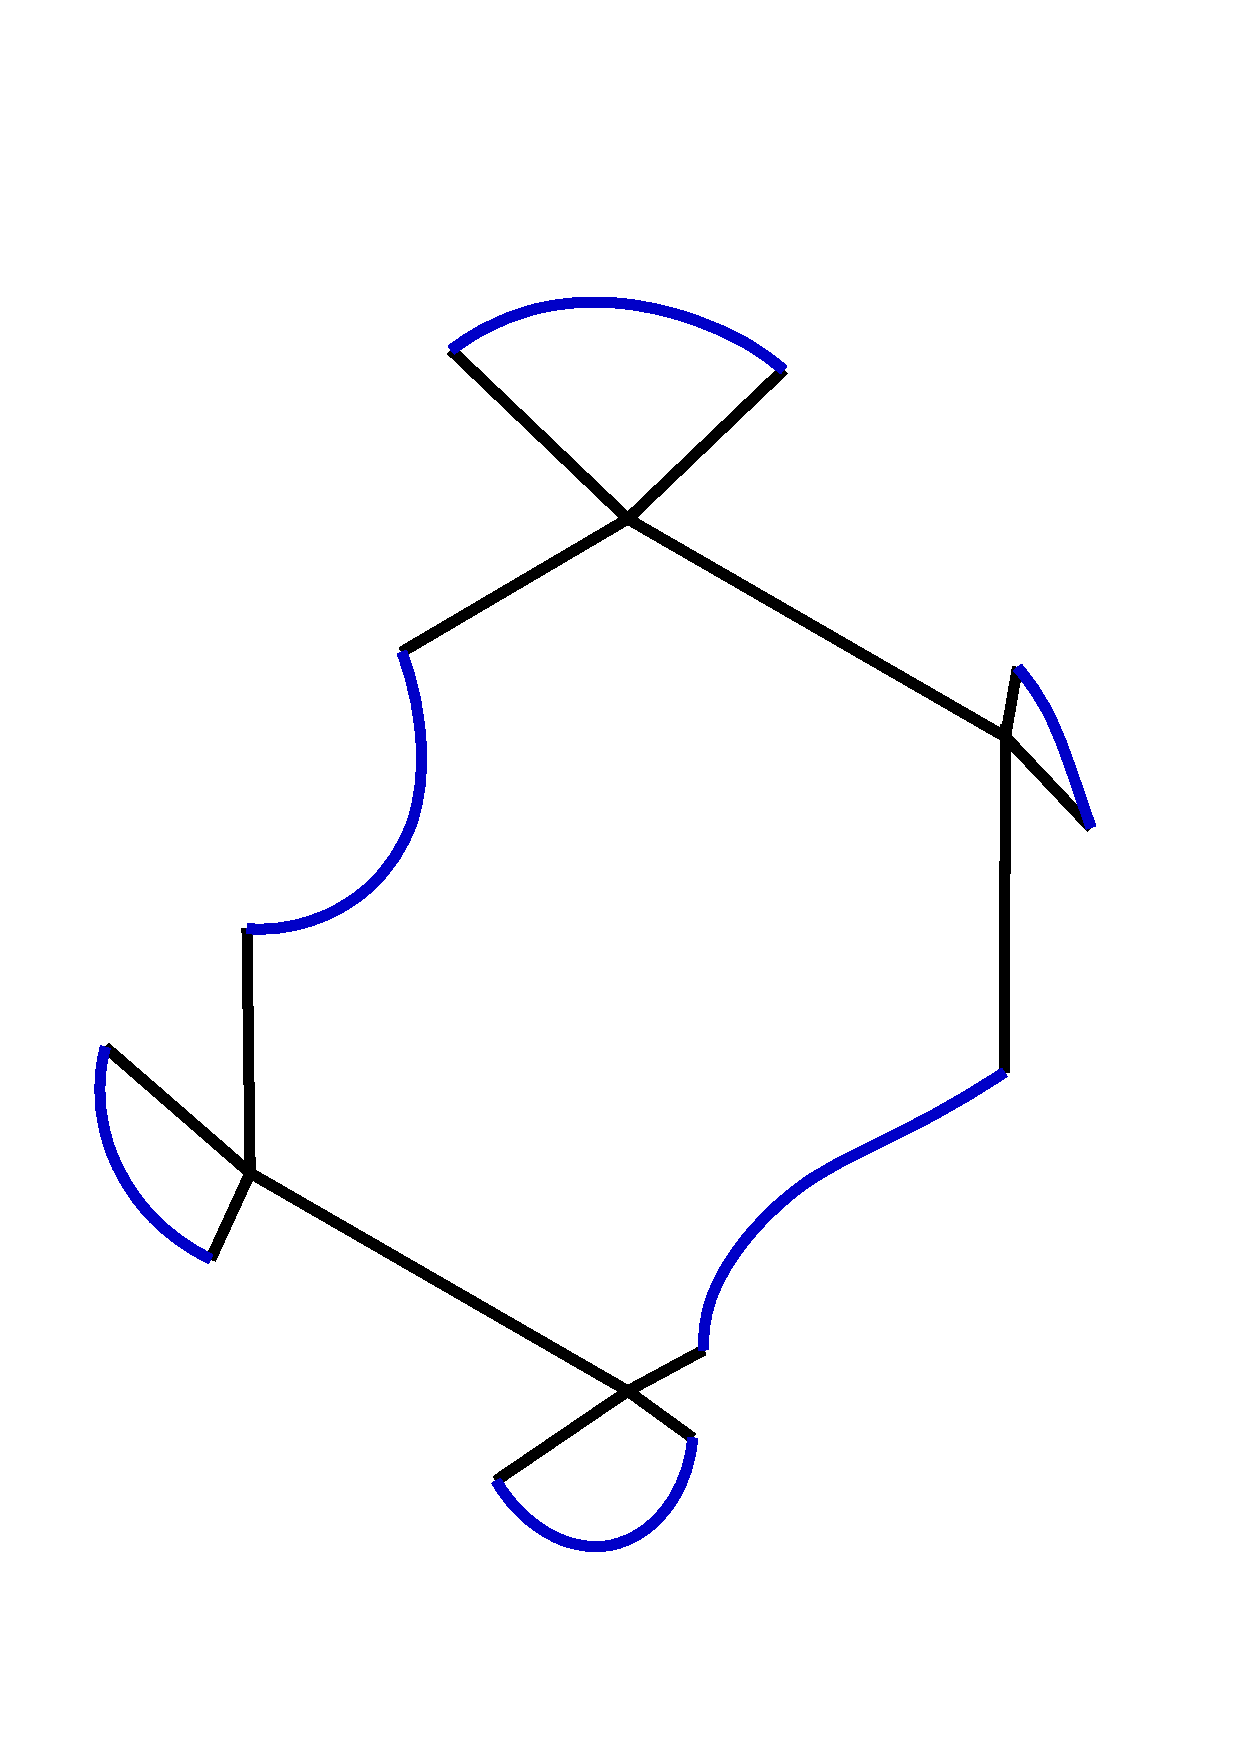
\includegraphics[scale=0.20]{multi_component_fig_5_crop}
    \caption{\label{fig:multicomponentc}}
  \end{subfigure}
  %\hspace*{.5in}
  \begin{subfigure}[t]{2in}
    \centering
    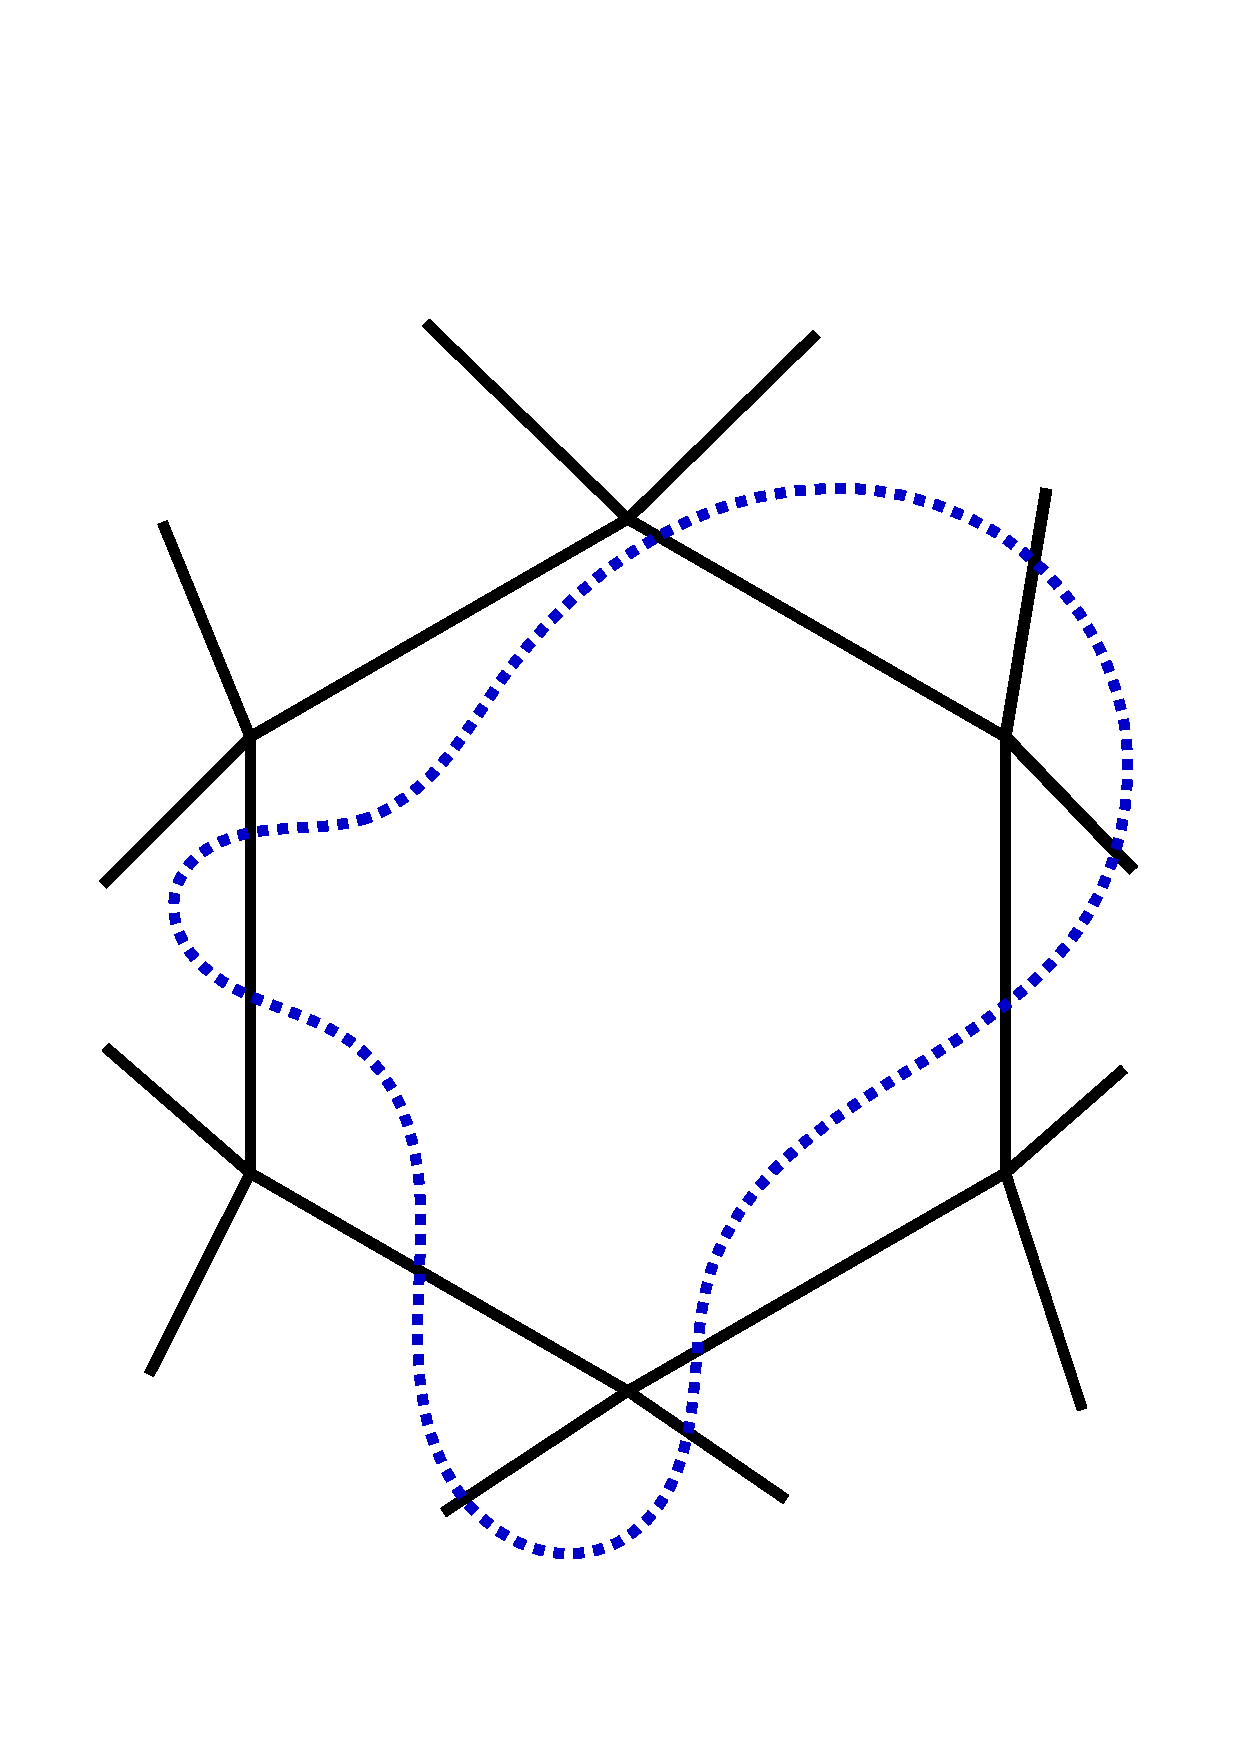
\includegraphics[scale=0.20]{multi_component_fig_3_crop}
    \caption{\label{fig:multicomponentd}}
  \end{subfigure}
  \begin{subfigure}[t]{2in}
    \centering
    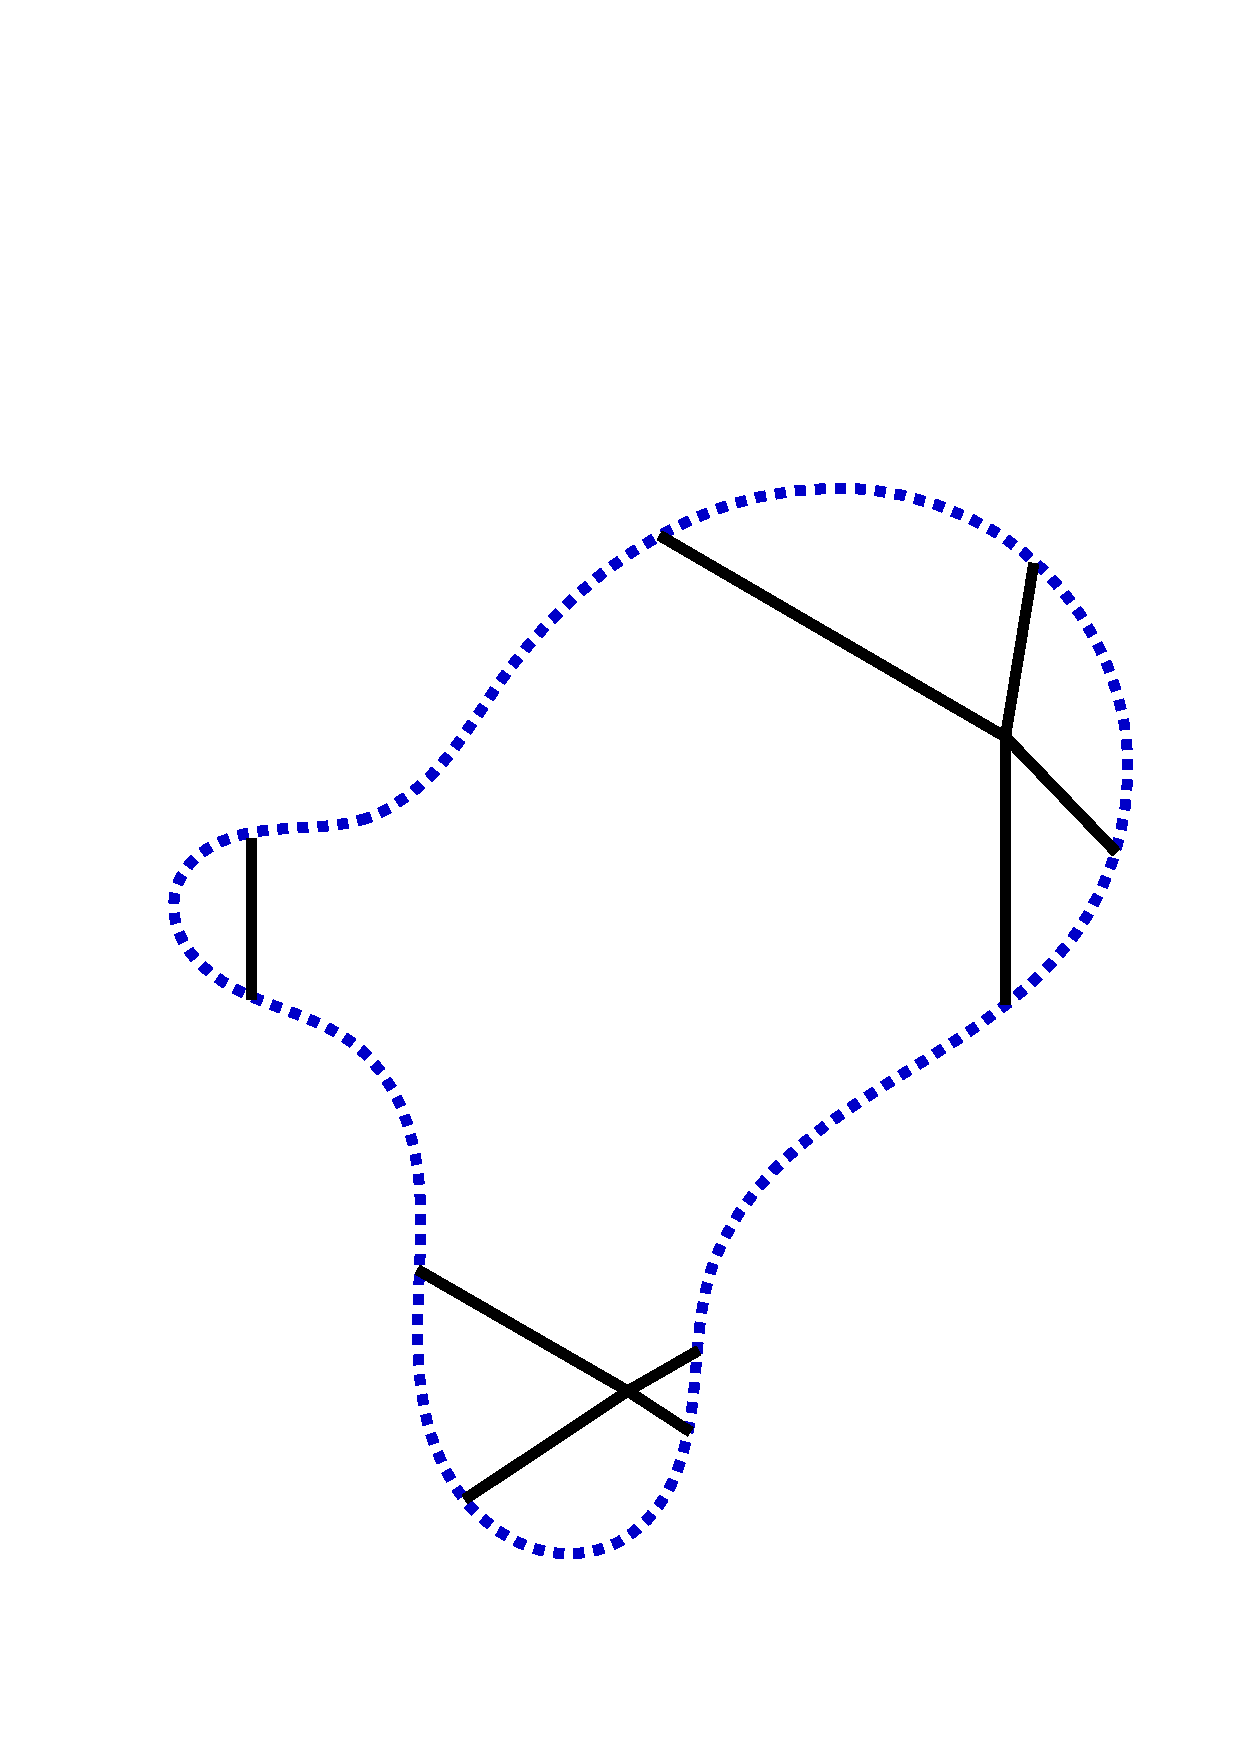
\includegraphics[scale=0.20]{multi_component_fig_4_crop}
    \caption{\label{fig:multicomponente}}
  \end{subfigure}
  %\hspace*{.5in}
  \begin{subfigure}[t]{2in}
    \centering
    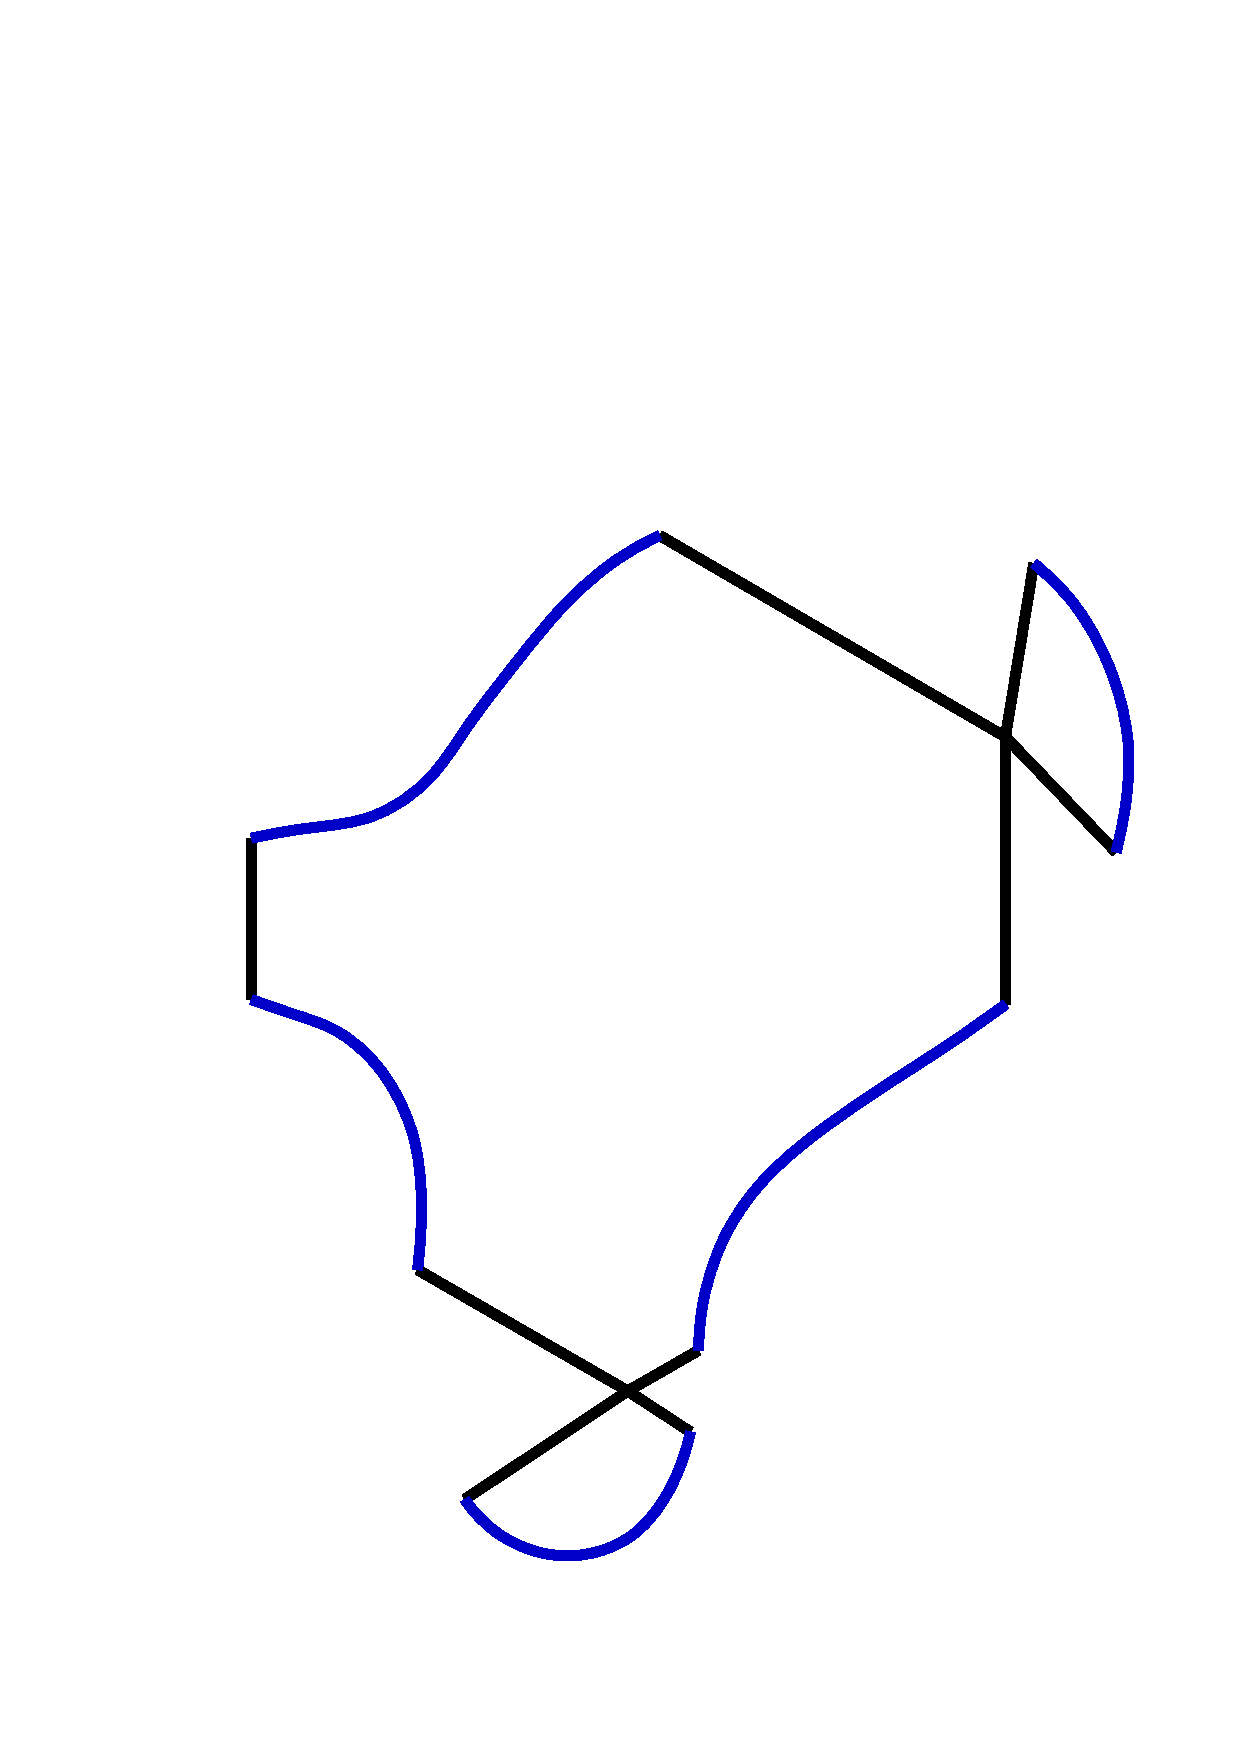
\includegraphics[scale=0.20]{multi_component_fig_6_crop}
    \caption{\label{fig:multicomponentf}}
  \end{subfigure}

  \caption{\label{fig:multicomponent}
    (a),(d) show one $2$-cell(Black) of complex $\hK$. Figure (b), (e) shows multiple components after \ref{def:clip} clip operation on $\hK$ with respective polygon(Dotted Blue) in some layer on Figure (a), (d). Figure (c), (f) shows \ref{def:patch} patch operation on Figure (b), (e) connecting multiple components with Solid Blue lines.}
\end{figure}

\begin{figure}[htp!] 
  \centering
  \begin{subfigure}[t]{1.6in}
    \centering
    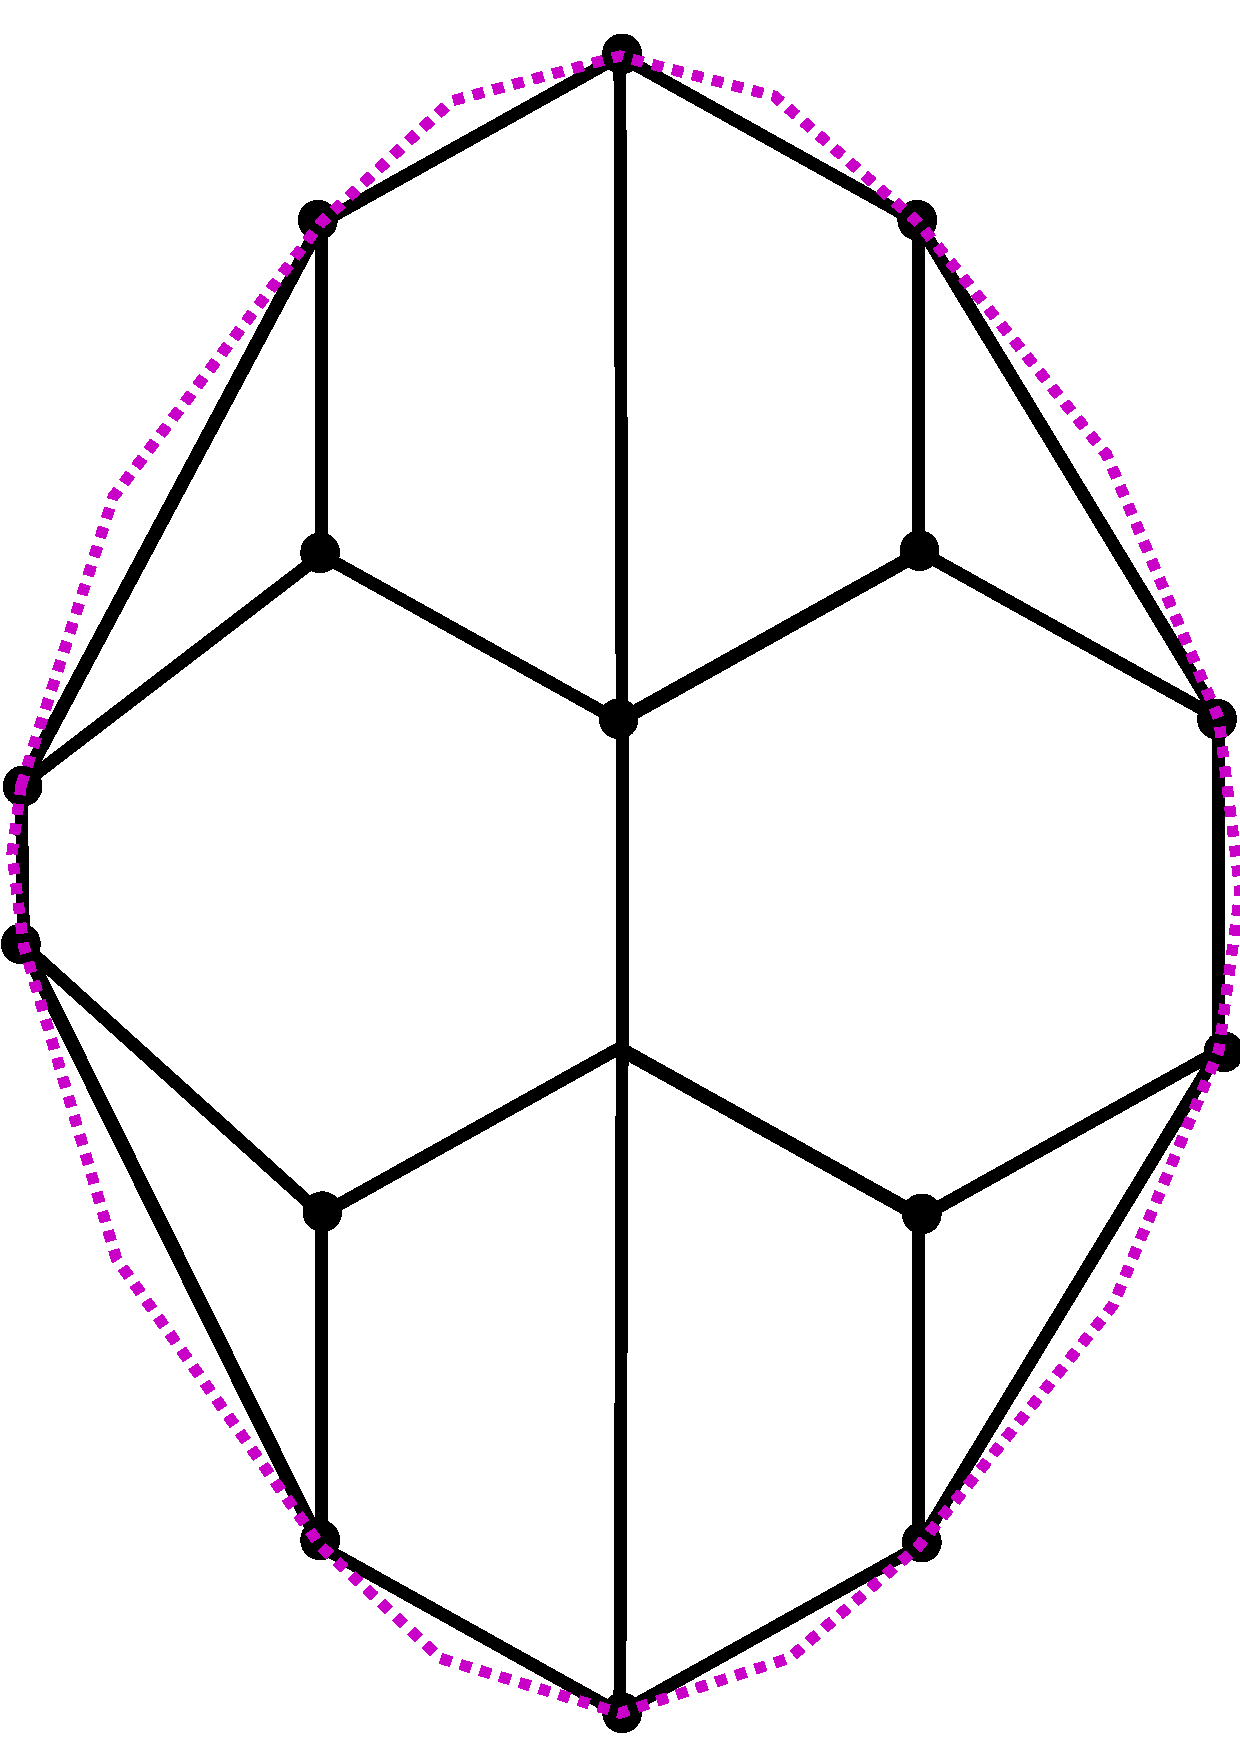
\includegraphics[scale=0.15]{infill_pattern_input_complex_scheme}
    \caption{\label{fig:printingprocessa}}
  \end{subfigure}
  \hspace*{0.3in}
  \begin{subfigure}[t]{1.6in}
    \centering
    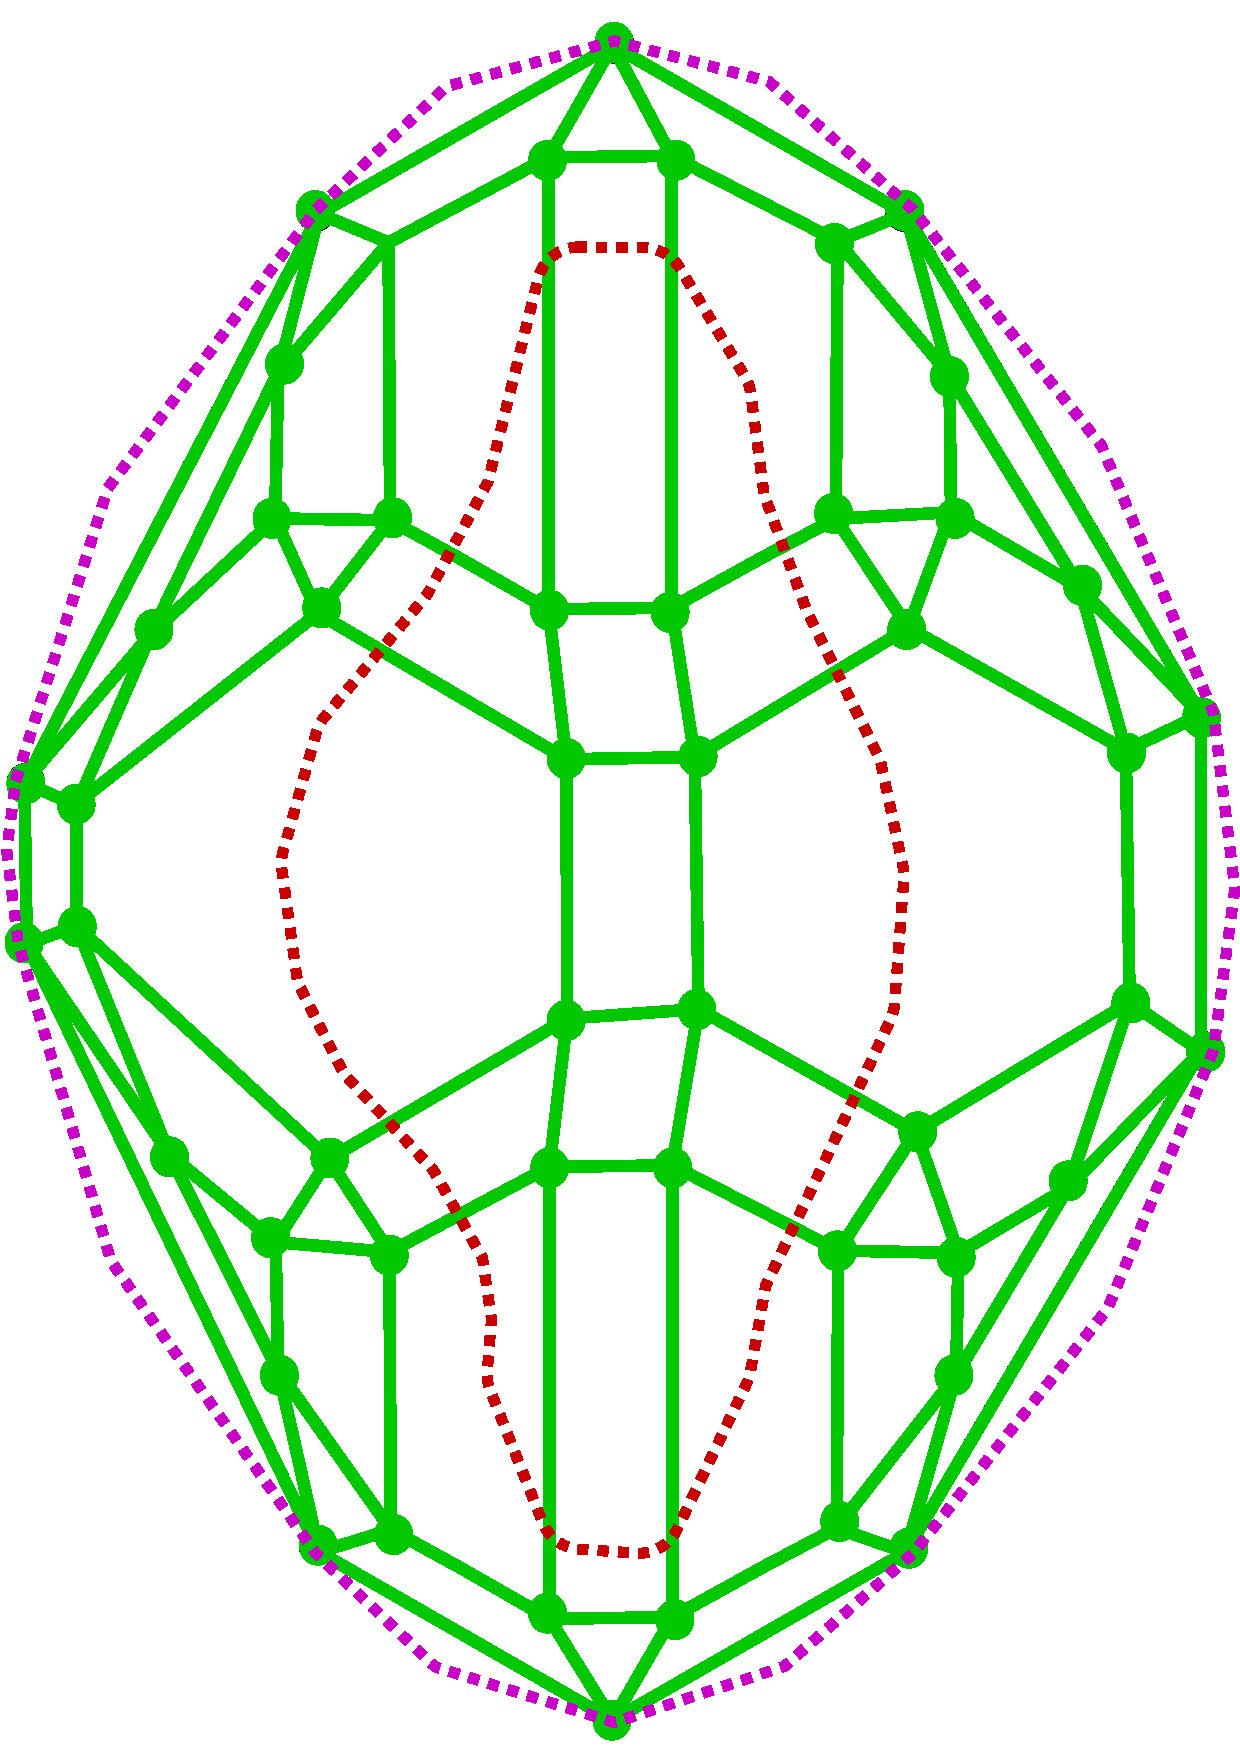
\includegraphics[scale=0.15]{infill_pattern_transformed_complex_scheme}
    \caption{\label{fig:printingprocessb}}
  \end{subfigure}	
  \begin{subfigure}[t]{1.6in}
    \centering
    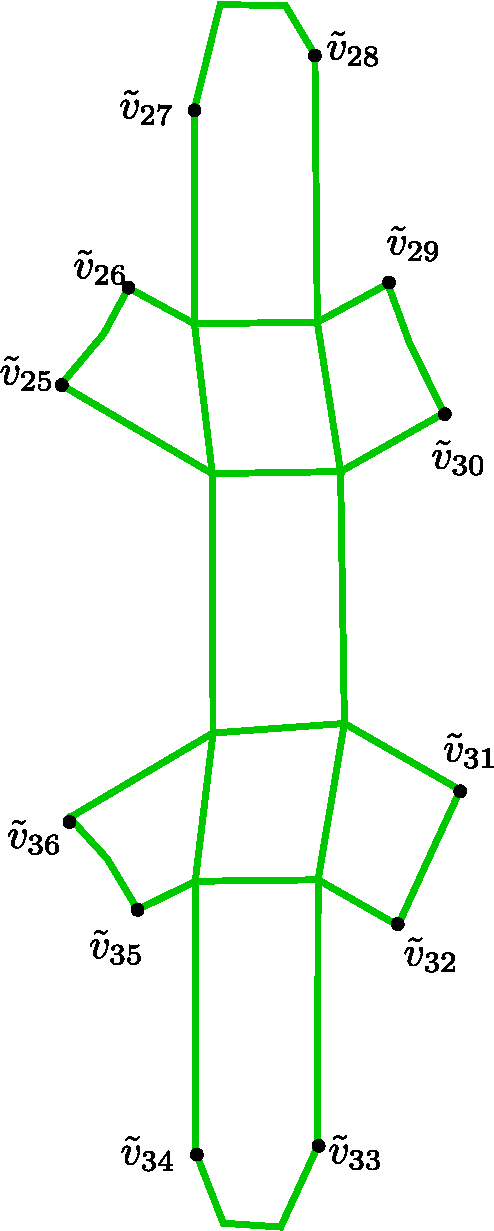
\includegraphics[scale=0.22]{infill_pattern_transformed_complex_cookie_cut_fig_8_crop}
    \caption{\label{fig:printingprocessc}}
  \end{subfigure}
  
  \caption{\label{fig:printingprocess}
    (a) Projected polygon $P$(purple) and initial $2$-complex K is in black. (b) Euler transformation $2$-complex $\hK$(green), Region $\tR_{ij}$(red dot) of some polygon $P_{ij}$. (c) $\hK$ is clipped using $\tR_{ij}$ and patched to $2$-complex $\tK$(green) after step \ref{itm:patch}, where $\tR_{ij}$ has  $\{\tv_1, \dots , \tv_{24}\}$ sequence of vertices and $\{\tv_{25}, ..... , \tv_{36}\}$ are points of intersection of $\tR_{ij}$ and $1$-skeleton of $\hK$.
  }
\end{figure}

\vspace*{-0.05in}
\subsection{Continuous Tool Path Planning Framework: Steps} \label{ssec:steps}
\vspace*{-0.05in}

Our framework for continuous tool path planning consists of the following steps.
\begin{enumerate}
  \item {\bf{\textit{Slicing:}}}
    Slice an STL file of the design.
    This step creates a sequence of layers, and each layer can have multiple polygons.
    Let $\Ps_i = \{P_{ij}\}$ be the set of all the polygons in layer $i$ with or without holes.
    We assume the layers generated by slicing are $\epsilon$-continuous.
    
  \item{\bf{\textit{Projecting:}}}
    Project all polygons $\{P_{ij}\}$ in each layer $\Ps_i$ on to the horizontal plane.
    Take the {\bfseries union} of all projected polygons (from all layers).
    This union can have an irregular shape depending on the input.
    %Also, the projection set could affect quality parameter of input complex $K$.
    Let $P$ be the convex hull of the union of projected polygons.
    Note that taking the convex hull will avoid irregularities.
    We are assuming the input design has a single component.
    If not, we can repeat the procedure for each component.

  \item{\bf{\textit{Meshing:}}}
    Mesh $P$ with a pure $2$-complex $K$.
    We assume $K$ satisfies \cref{asmn:Kholesoutside}.
    
  \item \label{itm:eulertransform}{\bf{\textit{Euler Transformation:}}}
    Apply Euler Transformation to $K$ to create $\hK$.
    We assume that the traversal of edges in $\hK$ will not be affected by extruder size considerations (see \cref{sec:boundaryedges}).
    
  \item\label{itm:patch}{\bf{\textit{Clipping:}}} 
    $\tK$ is a $2$-complex contained in $\tR_{ij}$.
    It is generated by clip (\cref{def:clip}) and patch (\cref{def:patch}) operations on $\hK$ with respect to $\tR_{ij}$ as illustrated in \cref{fig:printingprocess}.
    By \cref{lem:singlecomponent}, we get that $\tK$ is connected and its $1$-skeleton is Euler since $\hK$ has a single component and its $1$-skeleton is Euler. 
    There are two possible choices of pairing alternate vertices for patch operation.
    We can choose arbitrarily between them as long as $\tK$ is a single component. 
    
    Printing the infill lattice in each layer amounts to printing edges in the $1$-skeleton of $\tK$.
    We clip the $2$-subcomplex $\tK$ for each layer from $\hK$ to prevent printing in free space.
    Each edge is supported by an edge in the layer below it except for boundary edges in $\tK$.
    We will add a support perimeter to support boundary edges in $\tK$, as discussed in the next step. 
      
  \item\label{itm:support}
    {\bf{\textit{Support Perimeter:}}}
    Let $\tR_{ij} \in P_{ij}$ and $\tR_{i+1,j} \in P_{i+1,j}$ be such that $\tR_{i+1,j}$ is supported by $\tR_{ij}$ through $\epsilon$-continuity as shown in \cref{fig:step_6_reasoning}.
    There are two possible ways we can select alternate pairs of vertices for subcomplex $\tK$ to join in $\tR_{i+1,j}$: $\{\{12, 13\}, \{14, 15\}, \{16, 11\}\}$ or $\{\{11, 12\}, \{13, 14\}, \{15, 16\}\}$. % (see \cref{fig:step_6_reasoning}).
    Then the edges $\{12, 13\}$ in the first case and $ \{11, 12\}, \{13, 14\}$ in second case are not supported if $\{2, 3\},\{4, 5\}, \{6, 7\}, \{8, 9\},$ and $\{10, 1\}$ are the vertices pairs selected for $\tR_{i+1,j}$.
    To solve this problem we need a way to print all the edges at boundary of the polygons.
    \begin{figure}[htp!] 
  	\centering
  	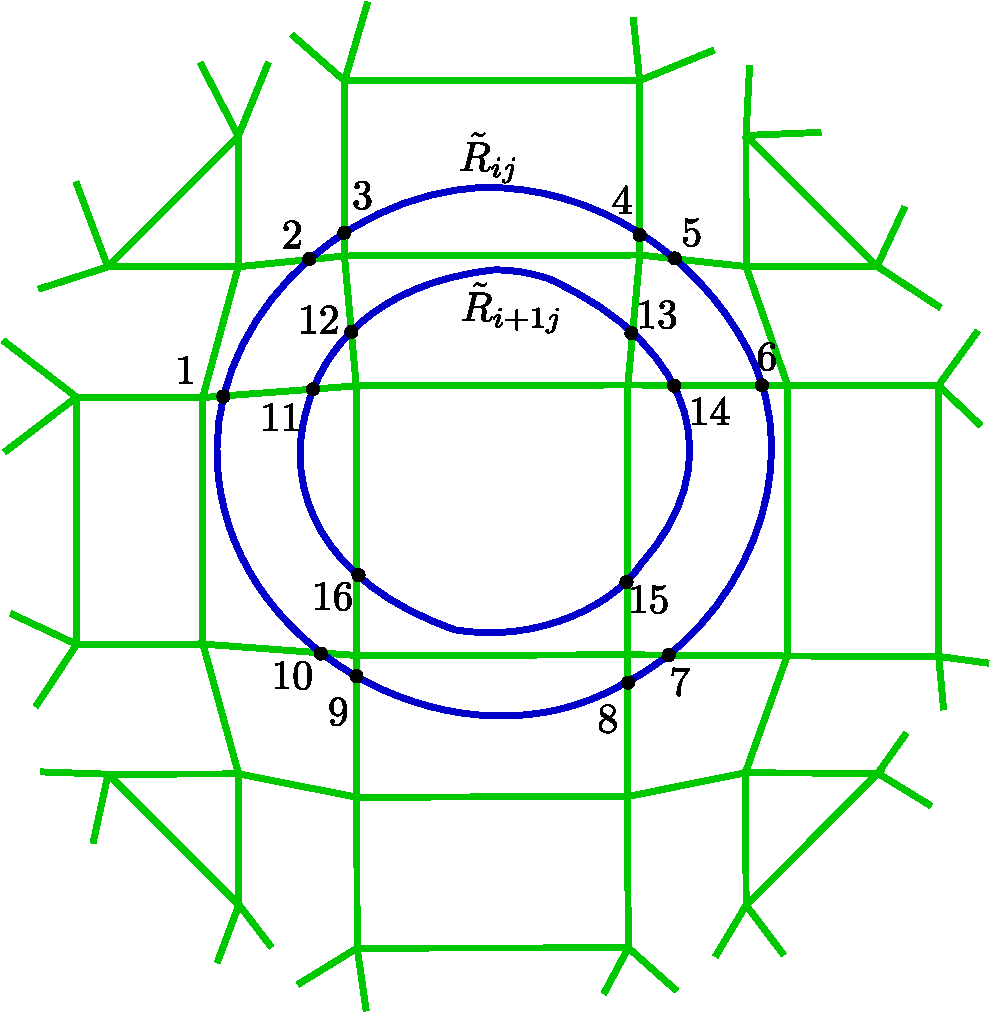
\includegraphics[width=50mm,height=50mm]{step_6_reasoning-crop}
  	\caption{\label{fig:step_6_reasoning}
          $\tR_{ij}$ (blue) in $P_i$, $\tR_{i+1j}$ (blue) in $P_{i + 1}$ intersect the complex $\hK$ (green) at points $\{1, \dots,10\}$ and $\{11, \dots, 16\}$, respectively.
        }
    \end{figure}  
  
    Since we are not printing all the edges at the boundary of $\tR_{ij}$, we could have some overhanging boundary edges in $\tK$.
    Let $\tP$ be the nonprinted path on $\tR_{ij}$ between $\tv_{n + l}$ and  $\tv_{n+l+1}$, which are vertices of $S$ on $\tR_{ij}$.
    Add circles of radius $r$, the extruder radius, on $\tv_{n+l}$ and $\tv_{n+l+1}$ and on path $\tP$ such that neighboring circles do not intersect.
    We assume the circles only intersect neighboring line segments on the path.
    Suppose $\eta$ is the maximum number of circles of radius $r$ that can be added on path $\tP$, assuming there are $2$ circles of radius $r$ centered at end points of the path.
    Add $\eta$ possible circles on path $\tP$, where the center of the $j^{\mbox{th}}$ circle is $\tv'_j$.
    The total gap we can have between the circles is $2r - \delta$, where $0 < \delta < 2r$ as shown in \cref{fig:supporta}.
    We can uniformly distribute the gap of $(2r - \delta)/(\eta + 1)$ between the circles as shown in \cref{fig:supportb} assuming $\eta$ is at least one.
    Since $\tR_{ij}$ is the inward Minkowski offset of $R_{ij}$ with a $2$-ball of radius $r$, for any $\tv'_j$ there exists a point $a$ such that line segment $\{\tv'_j, a\}$ is perpendicular to $\tR_{ij}$ and $R_{ij}$, and  $d(\tv'_j, a) = 2r$.
    Let $v_{n+k}$ and $v_{n+k+1}$ be points of intersection with $R_{ij}$ of the circle of radius $r$ centered at $a$.
    Create a corner by adding edges $\{v_{n+k}, a\}$, $\{v_{n +k +1}, a\}$ as shown in Figure \ref{fig:supportc}.
    Connect end points of the corners by a path on $R_{ij}$ if corner line segments do not intersect each other.
    Else change end points to the points of intersection so as to form a simple closed polygon as shown in \cref{fig:supportd}.
    We illustrate in \cref{fig:supportperimeter} the support perimeter around $\tK$ shown in \cref{fig:printingprocessc}.
    
 \begin{figure}[htp!]    
   %\hspace*{-0.8in}
   \begin{subfigure}[t]{3in}
     \centering
     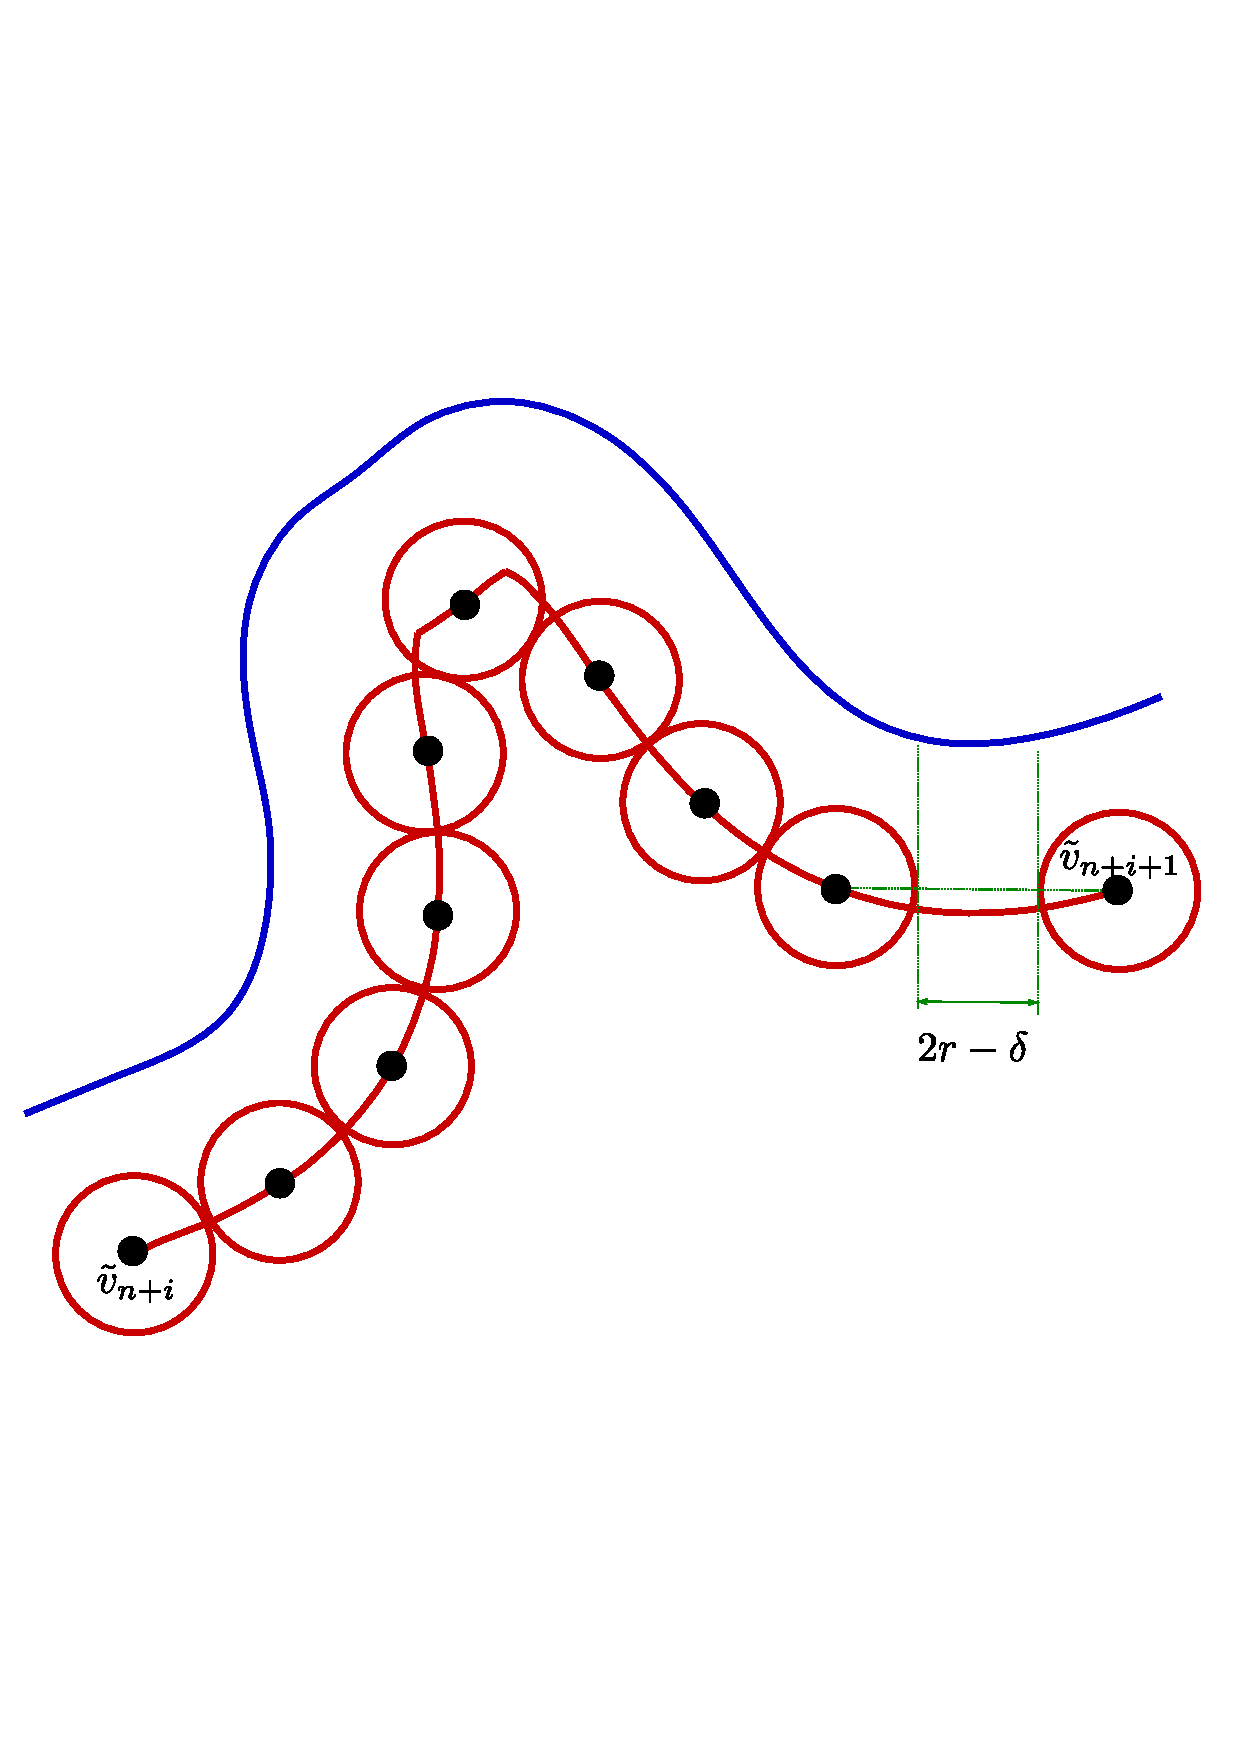
\includegraphics[scale=0.30]{support_fig_1_crop}
     \vspace*{-0.25in}
     \caption{\label{fig:supporta}}
   \end{subfigure}
   \begin{subfigure}[t]{3in}
     \centering
     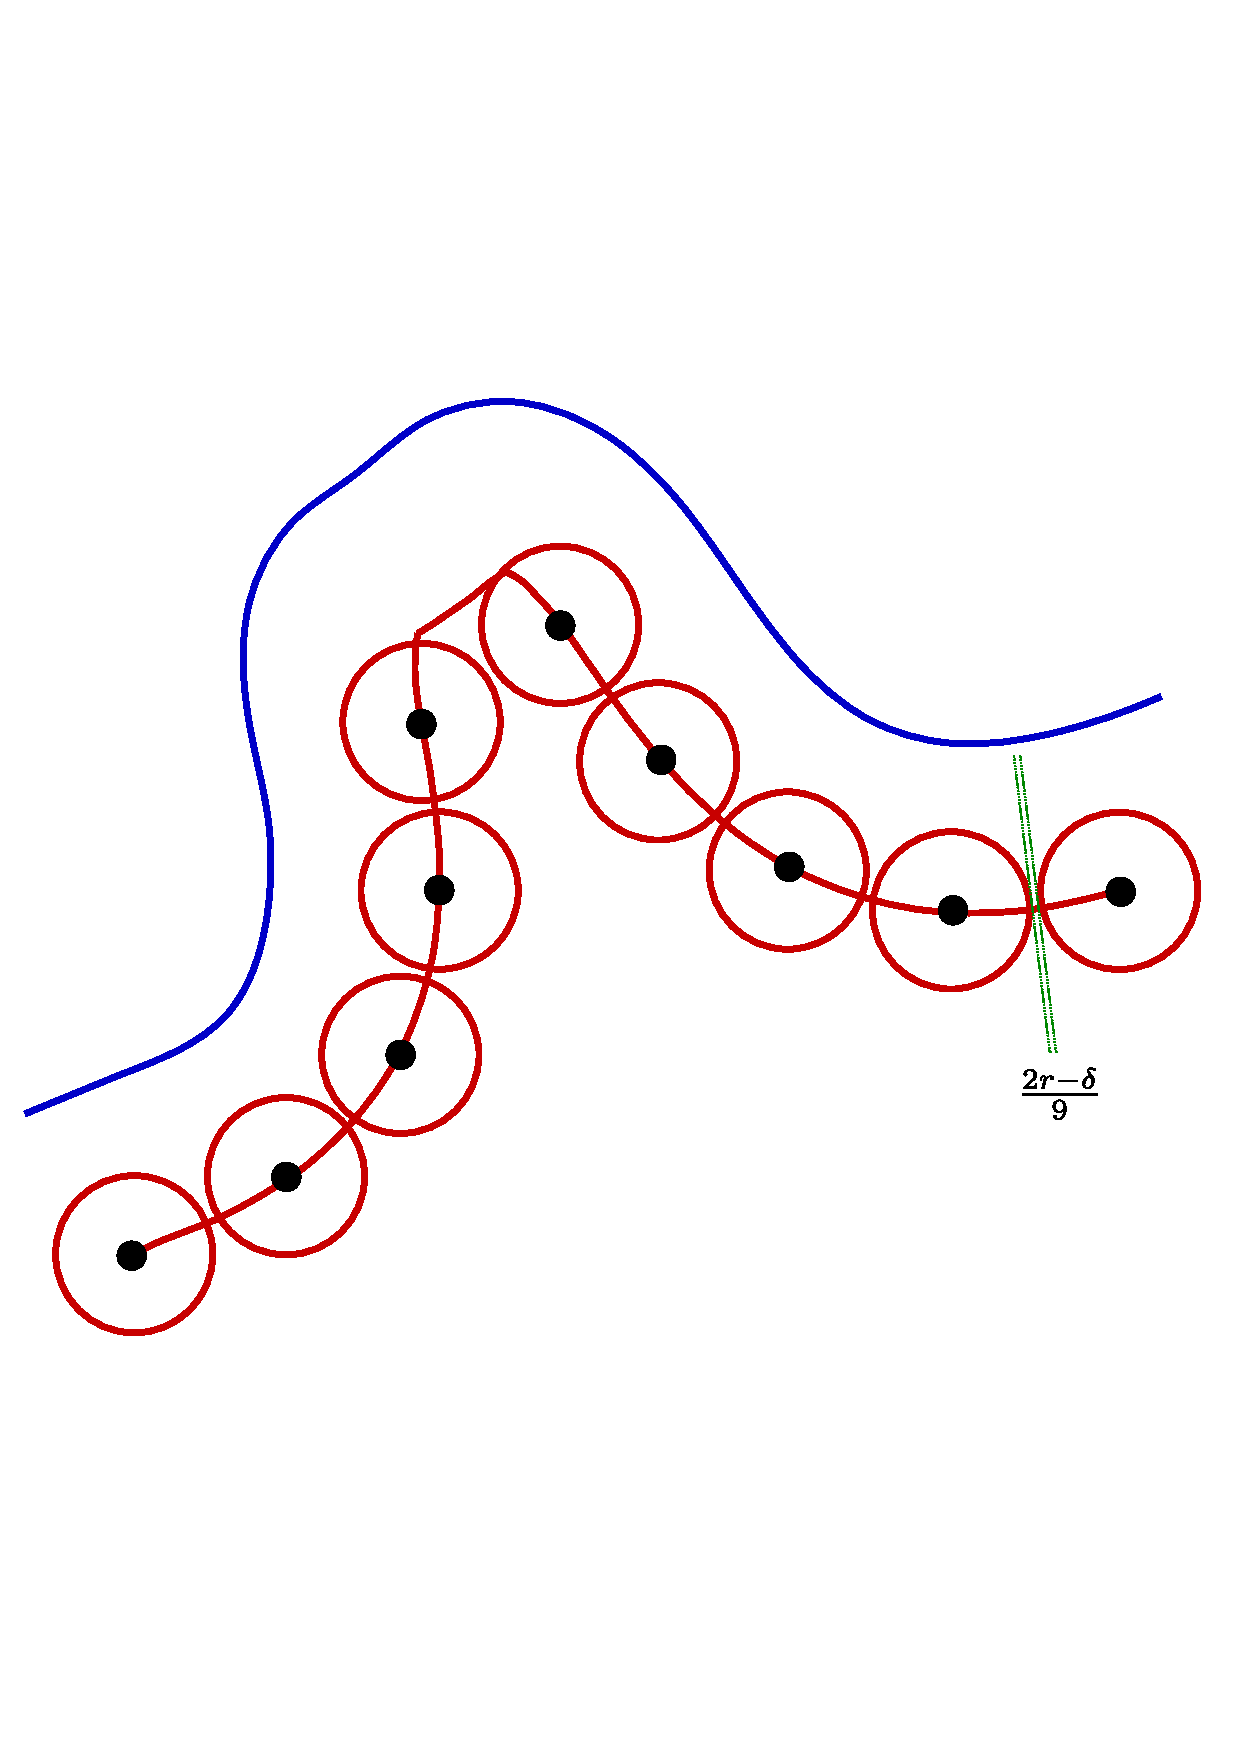
\includegraphics[scale=0.30]{support_fig_2_crop}
     \vspace*{-0.25in}
     \caption{\label{fig:supportb}}
   \end{subfigure}
 
   \begin{subfigure}[t]{3in}
     \centering
     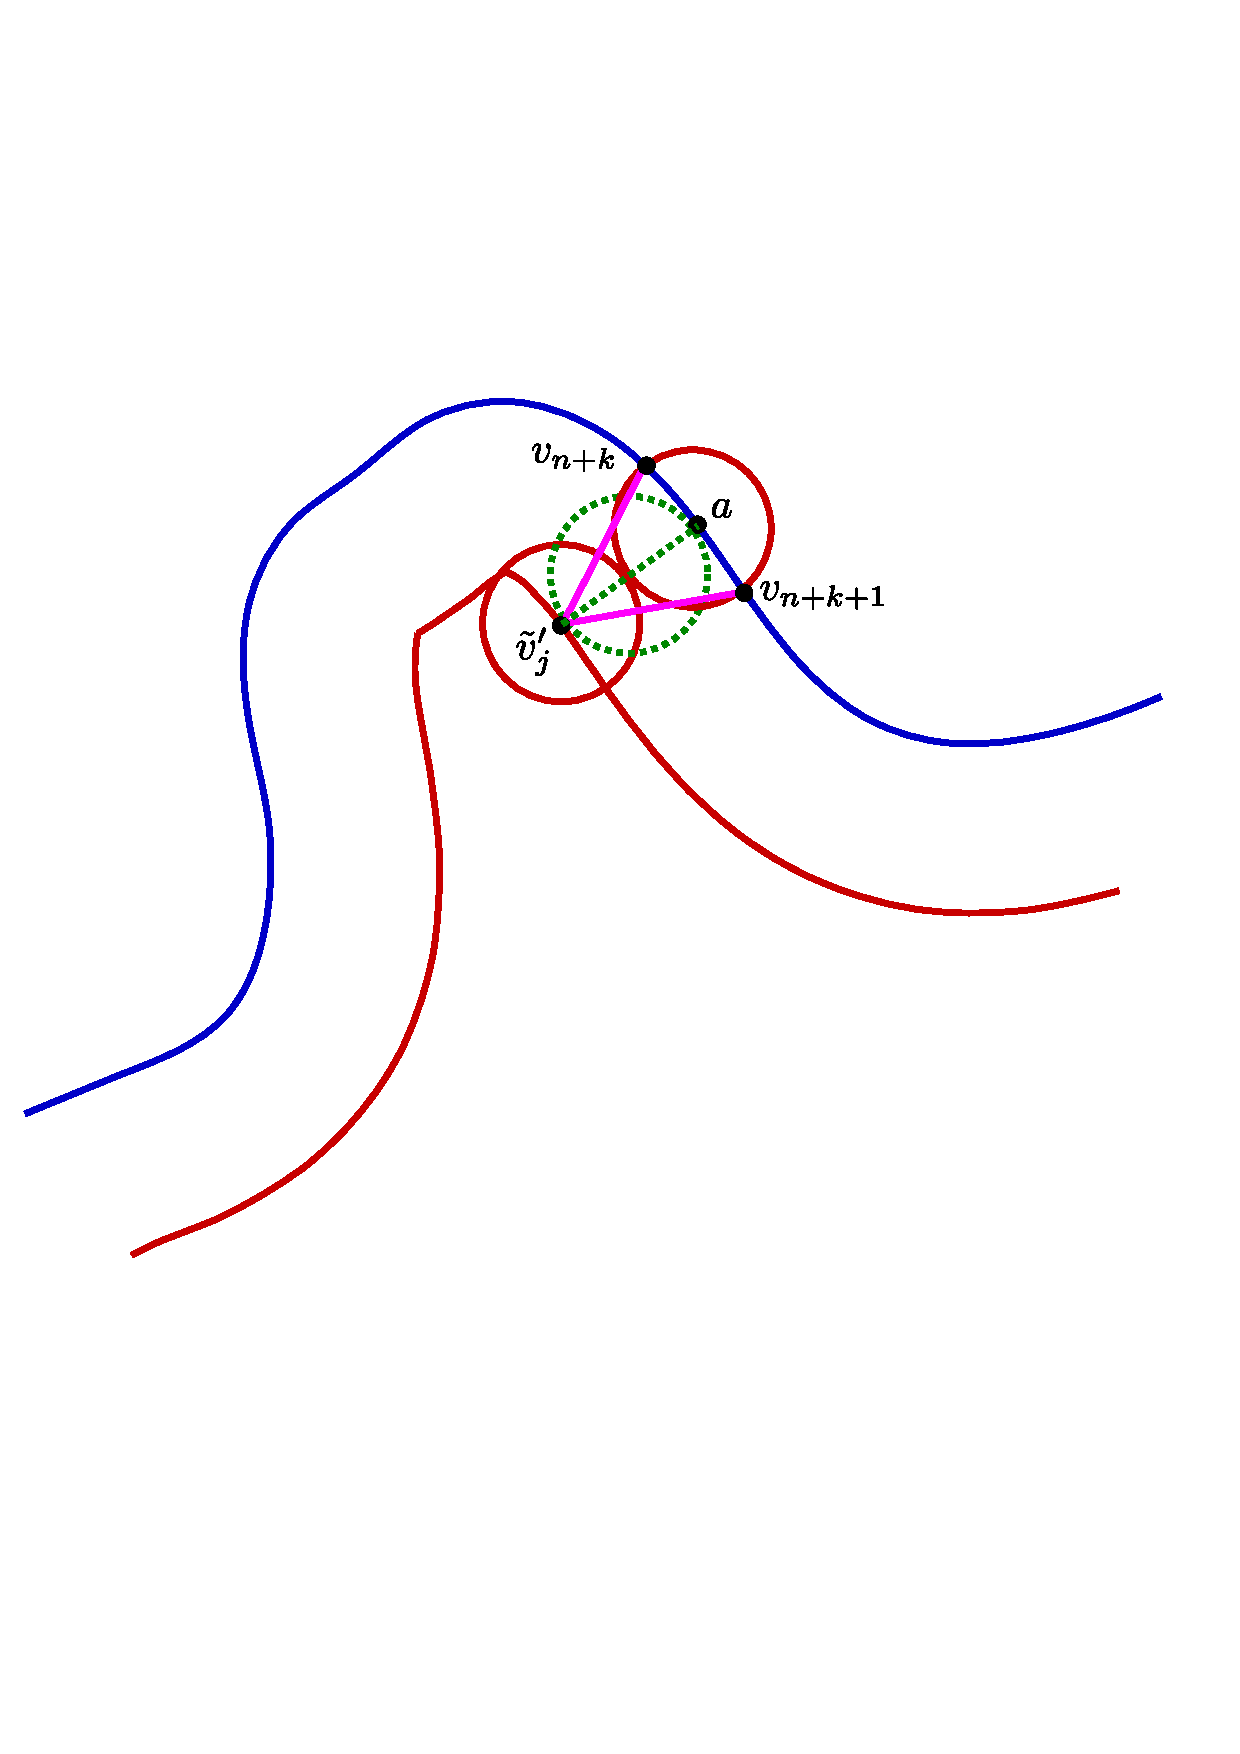
\includegraphics[scale=0.30]{support_fig_3_crop}
     \vspace*{-0.25in}
     \caption{\label{fig:supportc}}
   \end{subfigure}	
   \begin{subfigure}[t]{3in}
     \centering
     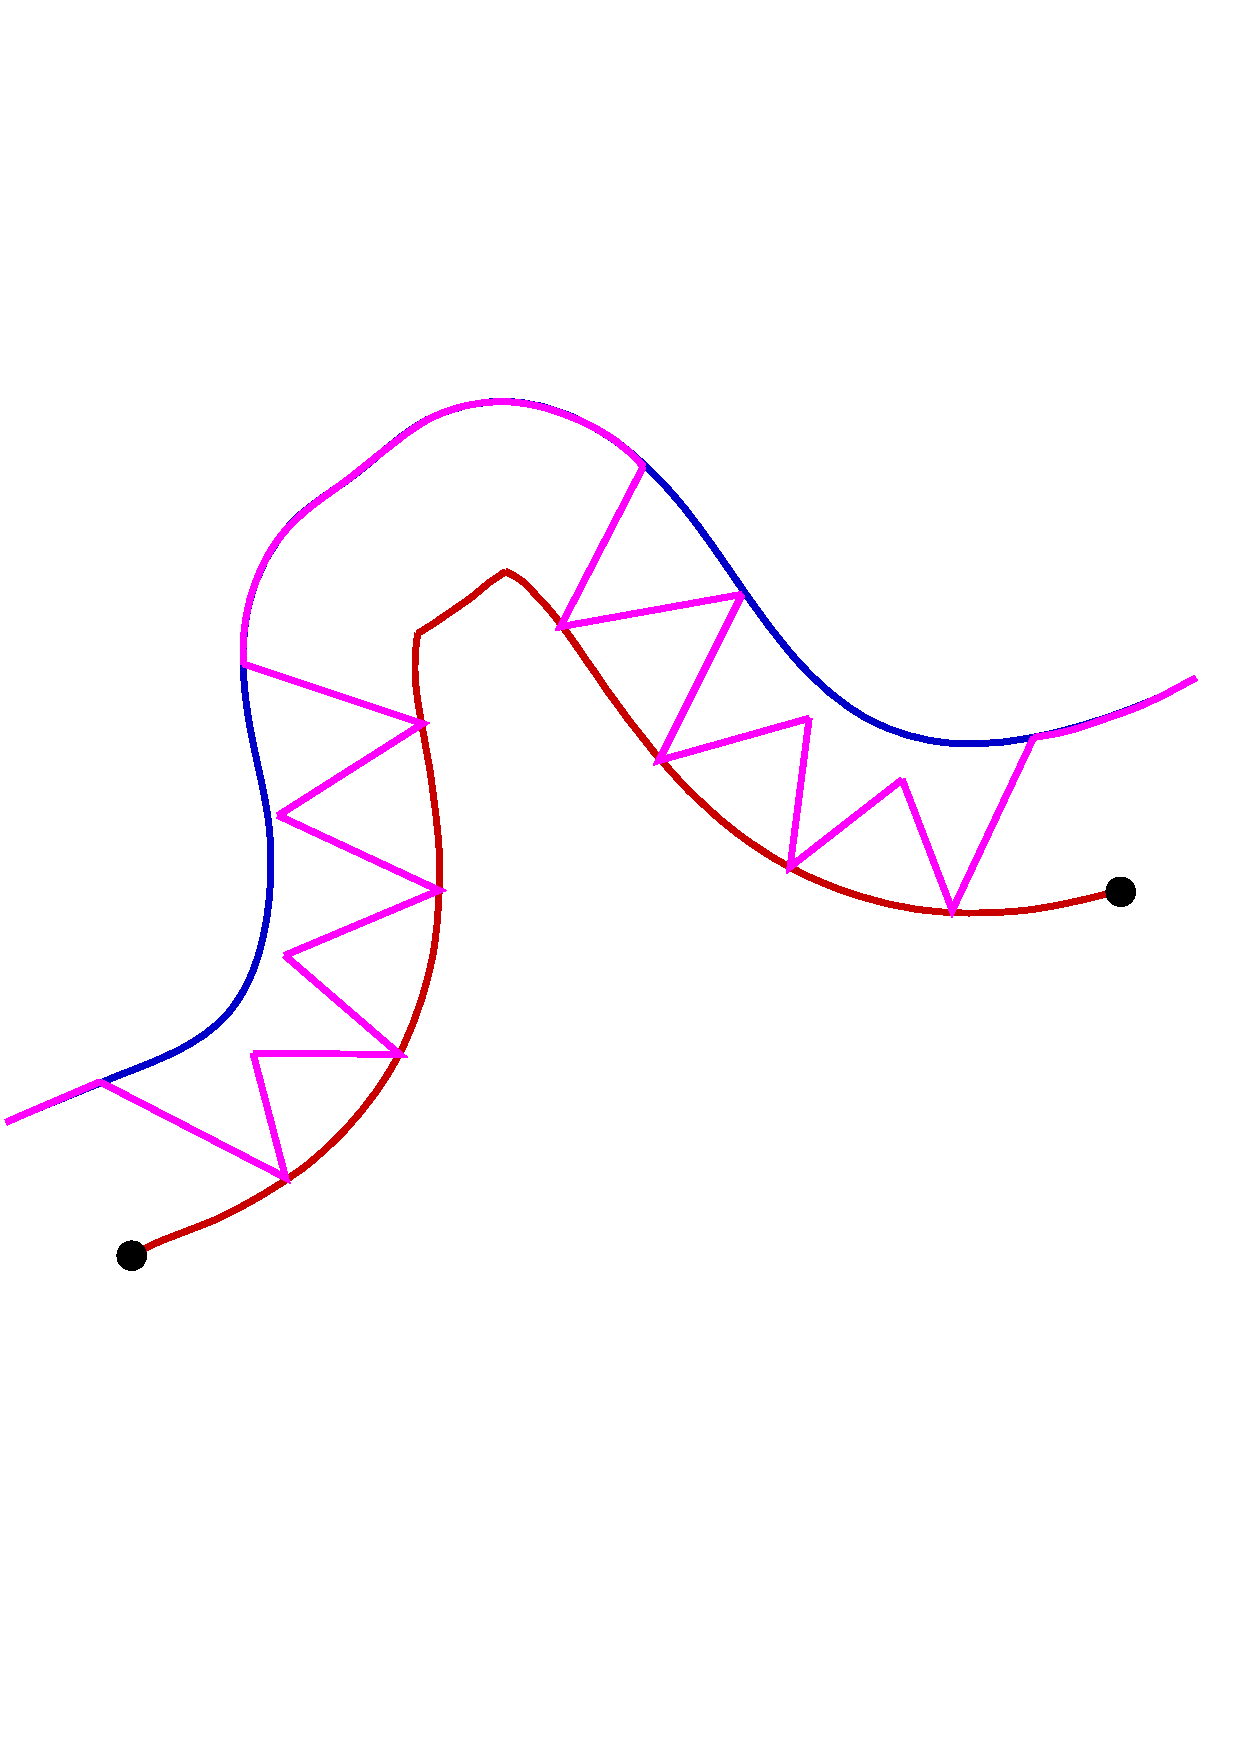
\includegraphics[scale=0.30]{support_fig_4_crop}
     \vspace*{-0.25in}
     \caption{\label{fig:supportd}}
   \end{subfigure}
   \caption{\label{fig:support}
     (a) Portion of $R_{ij}$ (blue) and $\tR_{ij}$ (red), $\tP$ (red), with total gap between circles being $2r - \delta$.
     (b) Uniformly distribute the gap between neighboring circles $\frac{2r - \delta}{9}$.
     (c) $\{v'_j, a\}$ is perpendicular to $\tR_{ij}$ and $R_{ij}$, circle centered at $a$ intersects $R_{ij}$ at $v_{n+k}, v_{n+k+1}$, and corner (pink) after adding edges $\{v'_j, v_{n+k}\}, \{v'_j, v_{n + k + 1}\}$.
     (d) Neighboring corners joined (pink) to form simple closed polygon.
     }
 \end{figure}    

 \begin{figure}[htp!] 
   \centering
   \vfill
   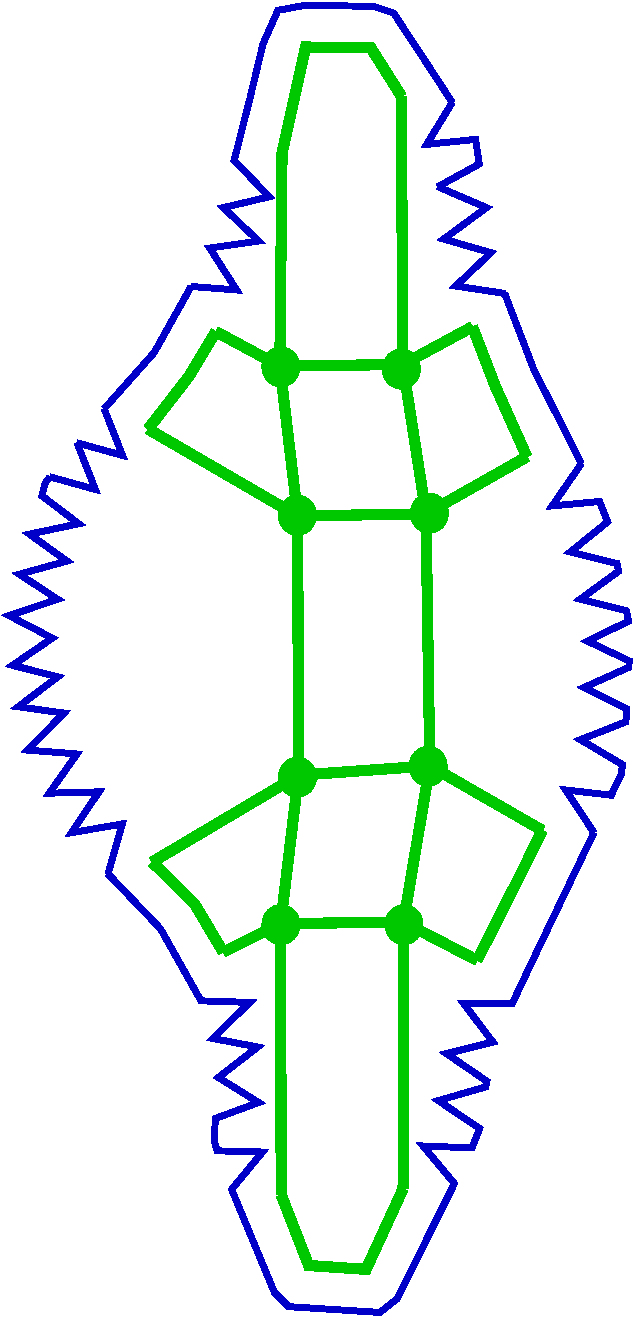
\includegraphics[scale=0.30]{infill_pattern_transformed_complex_cookie_cut_support_crop}
   \caption{Support perimeter for $\tK$ shown in \cref{fig:printingprocessc} is shown in blue here. }
   \label{fig:supportperimeter}
 \end{figure}   	 
\end{enumerate}


%\bigskip

\begin{rem}
  {\rm 
  In Step \ref{itm:support} above, we add corners only if we can add circles of radius $r$ on path $\tP$, given there are circles of radius $r$ at the end point of the path.
  It is not guaranteed that line segments of $\tP$ will be covered by the support, since the coverage depends on the curvature of $\tP$ as shown in Figure \ref{fig:supportd}.
  An alternative approach to printing the support is to print the individual non-printed sections in $\tR_{ij}$ while making non-print travel moves in between.
  But this approach will have $m/2$ starts and stops.
  If $\hK$ is a highly dense $2$-complex, then $m$ will be large and we will have a large number of starts and stops in this case.
  }
\end{rem}

\begin{rem}
  {\rm
    A continuous tool path exists only if any polygon in $\tK$ is shrinkable (\cref{def:shrinkable}) with no topological changes.
    But boundary polygons in $\tK$ due to clip and patch (\cref{def:clip,def:patch}) operations can be shrinkable with topological changes or unshrinkable as mentioned in \cref{sec:boundaryedges}.
  }
\end{rem}

\section{Generalized Euler Transformation} \label{sssec:genET}
We now consider generalizations of the Euler transformation where we could relax some of the assumptions we make on the input complex (\cref{asmn:Kholesoutside}).
We eventually want to allow combinatorial and topological changes in the polygons undergoing transformation.

Consider a $2$-complex $K$ consisting of a single polygon $f$.
$K$ does not satisfy the input condition for Euler transformation, since adjacent edges are shared with the outside (Figure \ref{fig:2cellpartition}).
Nevertheless, we apply the transformation to $K$.
In the resulting $\hK$, all vertices will have odd degree (circled in Figure \ref{fig:2cellpartition}).
But this $\hK$ satisfies the input condition, since any pair of adjacent edges of a polygon in $K$ now belong to two new polygons in $\hK$.
Hence if we apply the Euler transformation again to $\hK$, i.e., we apply it \emph{twice} on $K$, the resulting complex has a $1$-skeleton that is Euler in the default setting (without combinatorial and topological changes in class-$1$ polygons), even if adjacent edges of a polygon in $K$ are boundary edges.
More generally, we define this process as the generalized Euler transformation.

\begin{defn}
	\label{def:genET}
	(Generalized Euler Transformation in $d=2$)
	Let $K$ be a $2$-dimensional cell complex in $\R^2$ with polygons possibly having adjacent boundary edges.
	Apply the Euler transformation on $K$ to obtain $\hK$, even if $K$ do not satisfy input conditions \ref{asmn:Kholesoutside}.
	$\hK$ will always satisfy \cref{asmn:Kholesoutside}, so now apply Euler transformation on $\hK$.
\end{defn}
We could use the generalized Euler transformation to improve mechanical properties of the design (by increasing the density of the mesh) in some regions while still guaranteeing that the $1$-skeleton of the $2$-complex is Euler.
Notice that the density of the mesh is increased by this process, as shown in following result. 
\begin{lem}
  \label{lem:trgrrate} 
  After $m$ rounds of transformation of input complex $K$, the number of vertices $|\hat{V}^m| = 2\cdot 4^{m-1}|E|$ and number of edges $|\hat{E}^m|=4^m|E|$.	
\end{lem}
\begin{proof}
  After the first transformation, we get $|\hat{E}^{1}| = 4 |E|$ (by \cref{lem:cntshVhEhF2d}).
  And after the second transformation we get $|\hat{E}^2| = 4 |\hat{E}^1| = 4^2|E|$.
  Extending the argument, after $m$ transformations we get $|\hat{E}^m| = 4^m |E|$.
  Similarly, we get $|\hat{V}^1| = 2 |E|$, then $|\hat{V}^m| = 2 |\hat{E}^{m-1}| = 2\cdot4^{m-1}|E|$.     	
\end{proof}
The above result shows that the numbers of vertices and edges grow significantly after each iteration of transformation.
Hence the generalized Euler transformation may create a large number of edges.

We now discuss Euler transformation with \emph{combinatorial} and \emph{topological} changes to a polygon resulting from its mitered offset. 

\subsection{Euler Transformation with Combinatorial changes}\label{sec:eulertransformwithcombin}

Suppose $\hf, \hf_e, \hf_v$ are $3$ classes of polygons corresponding to a polygon ($f$), edge ($e$), and a vertex($v$) in $K$.
Maximum mitered offset in a polygon of the input complex $K$ is limited by the smallest edge length, as the mitered offset in our original Euler transformation assumes no combinatorial and topological changes in $\hf$.
\textit{Combinatorial change in $\hat{K}$ is a change in number of edges of some class-$1$ polygon $\hat{f}$ in $\hat{K}$ from corresponding polygon in $f$ in $K$.} 
Suppose polygon $f$ has $n$ edges and is now permitted to have combinatorial changes when generating its mitered offset.
Then we can reduce at most $n-3$ edges as we want $\hf$ to still be a polygon, and a polygon has at least $3$ edges.
If $\hf_e$ is sharing edges with two Class $1$ polygons and if both of those edges are reduced, then $\hf_e$ will collapse into an edge as shown in Figure \ref{fig:eulertransfecollapse}.
Since Class $3$ polygons ($\hf_v$) do not share edges with any Class $1$ polygons, combinatorial changes in the Euler transformation will not affect the number of edges in $\hf_v$.
%
\begin{figure}[ht!] 
  \centering
  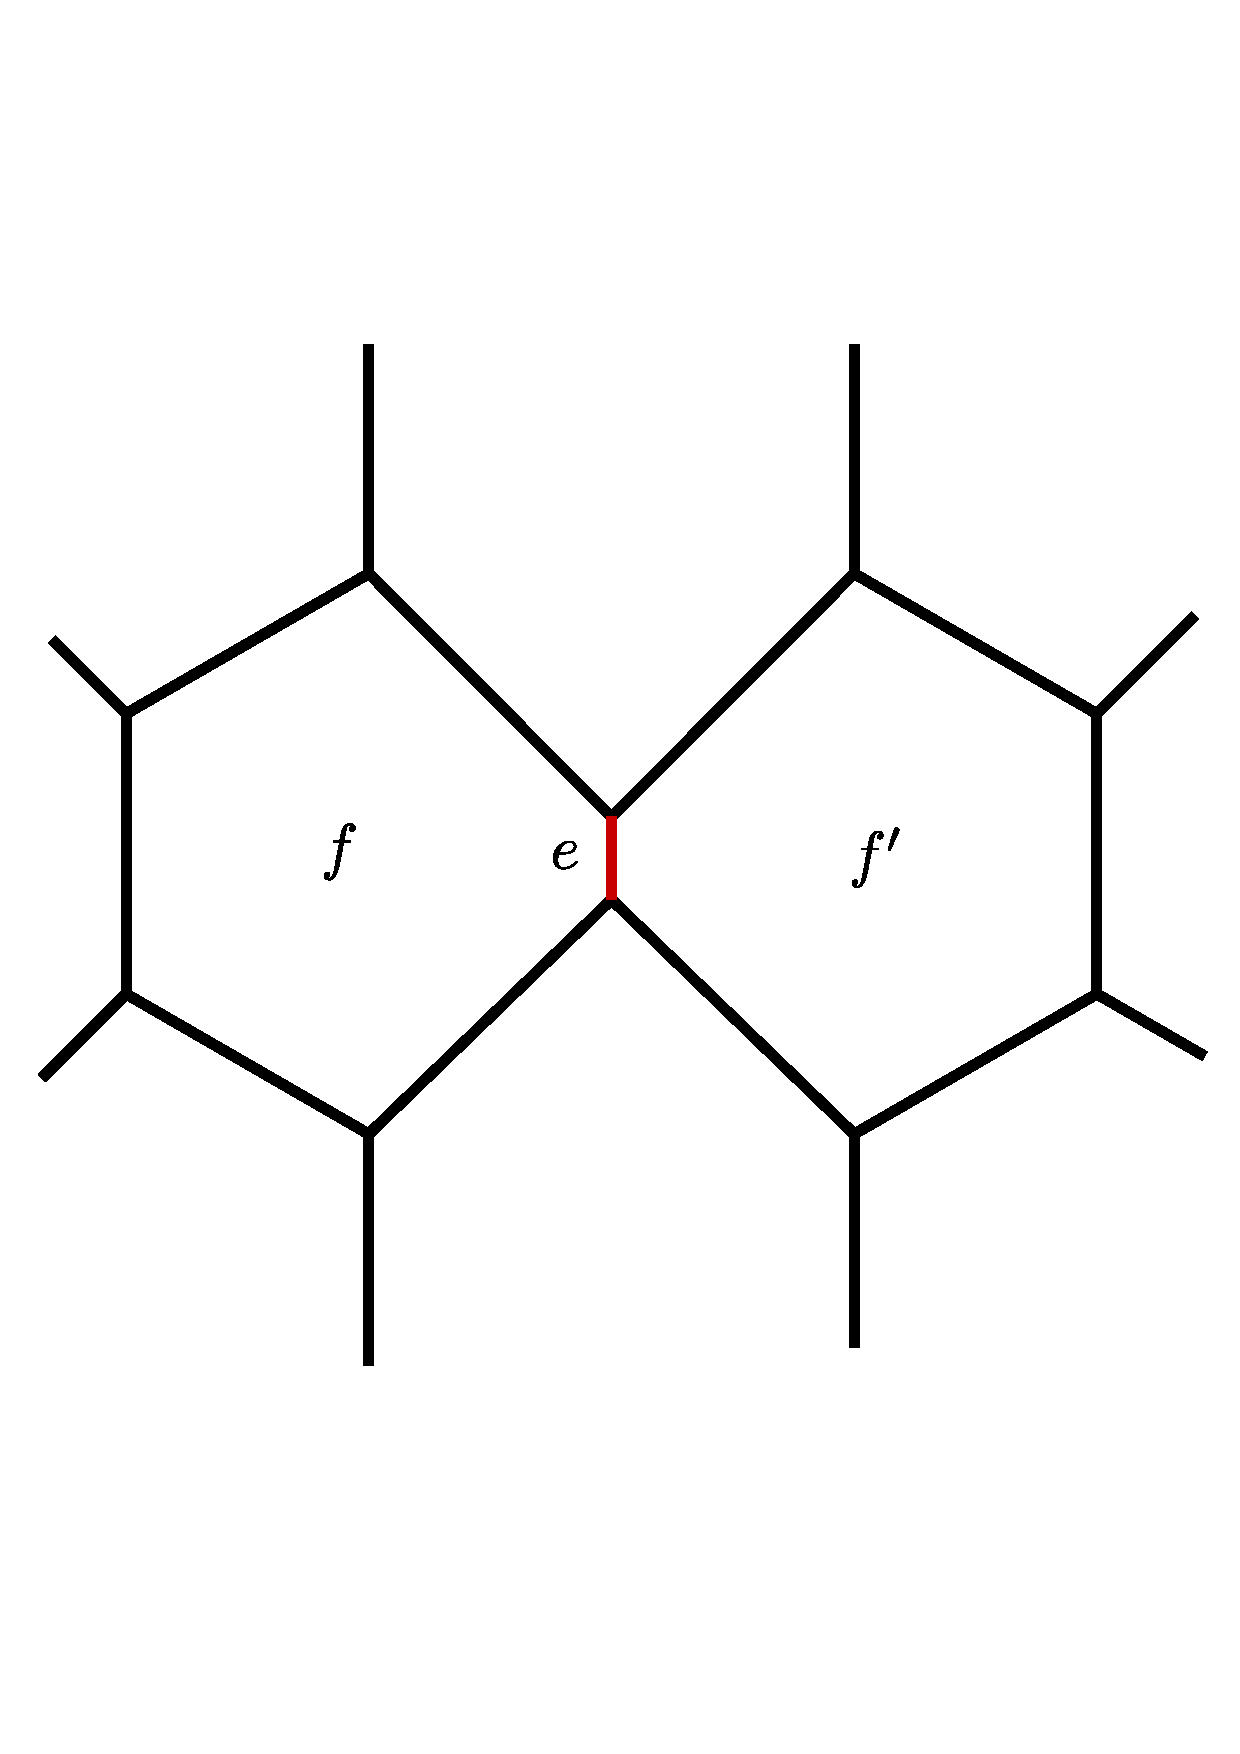
\includegraphics[scale=0.20]{input_complex_combinatorial_change_class_2_cell_collapse_fig_1_crop}
  \quad
  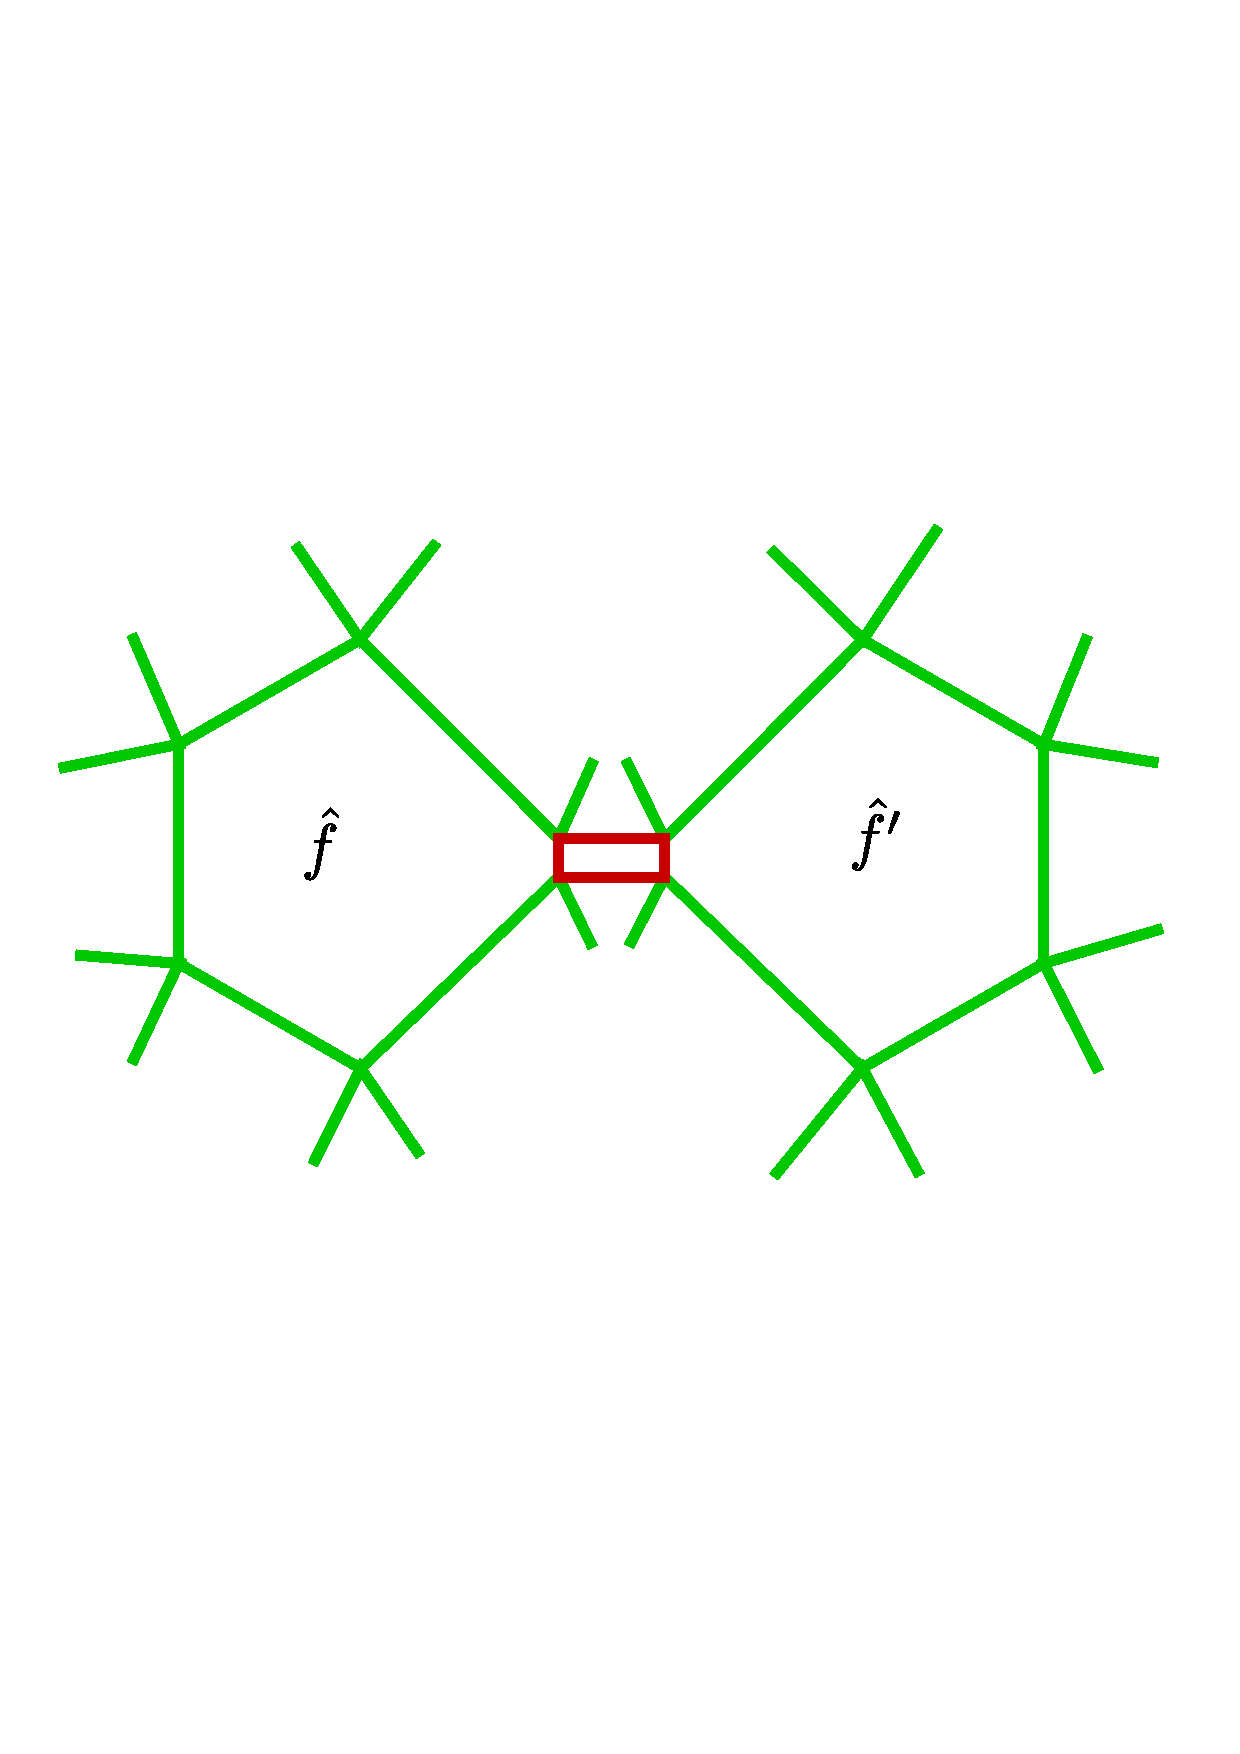
\includegraphics[scale=0.25]{intermediate_complex_combinatorial_change_class_2_cell_collapse_fig_1_crop}
  \quad
  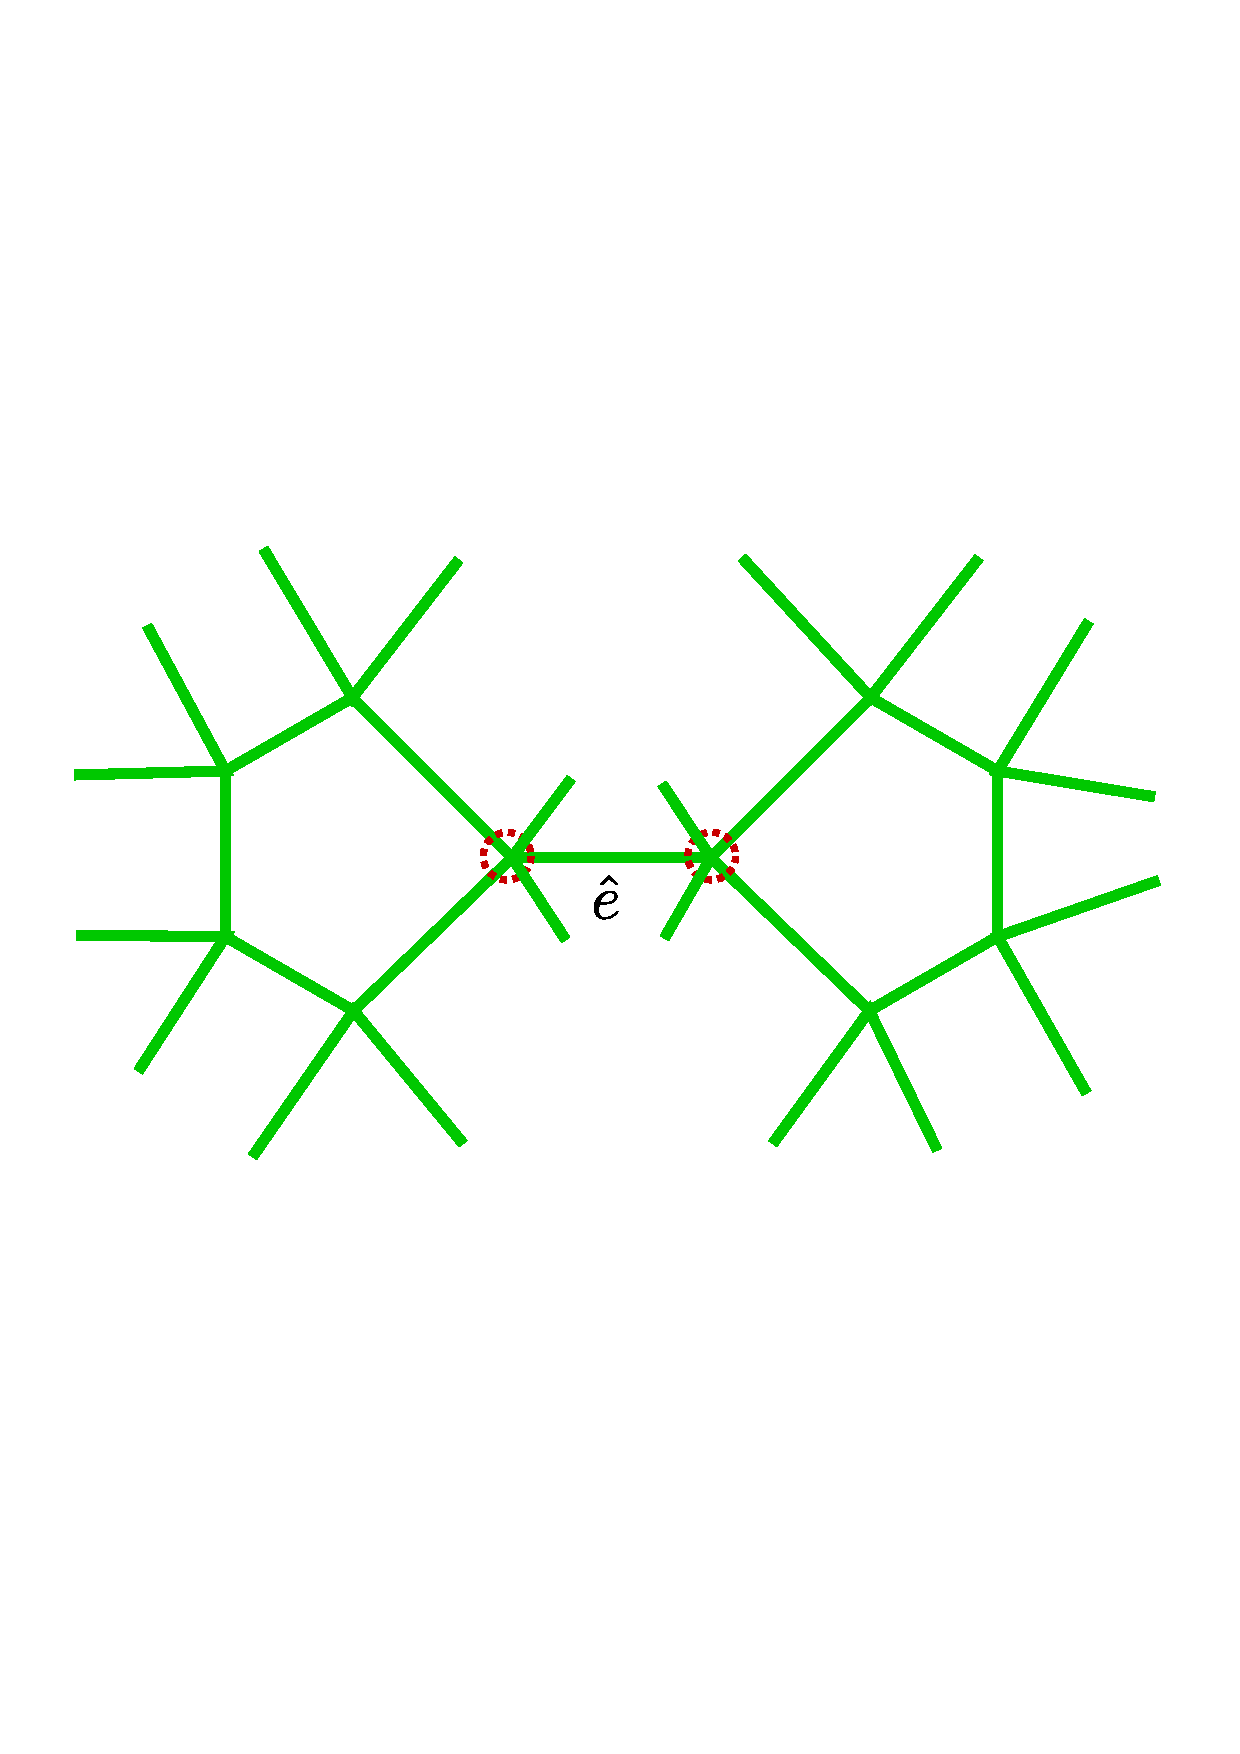
\includegraphics[scale=0.25]{output_complex_combinatorial_change_class_2_cell_collapse_fig_1_crop}
  \caption{\label{fig:eulertransfecollapse}
    Two polygons of a $2$-complex $K$ in the plane (top).
    Euler transformation of $K$ into $\hK$ (middle), where $\hf, \hf'$ are Class $1$ polygons and $\hf_e$ (red) is a Class $2$ polygon corresponding to edge $e$ (red) in $K$.
    Class $2$ polygon $\hf_e$ is collapsed to an edge $\he$ and red circled vertices have odd degree (bottom).
  }
\end{figure}

\begin{figure}[htp!] 
	\centering
	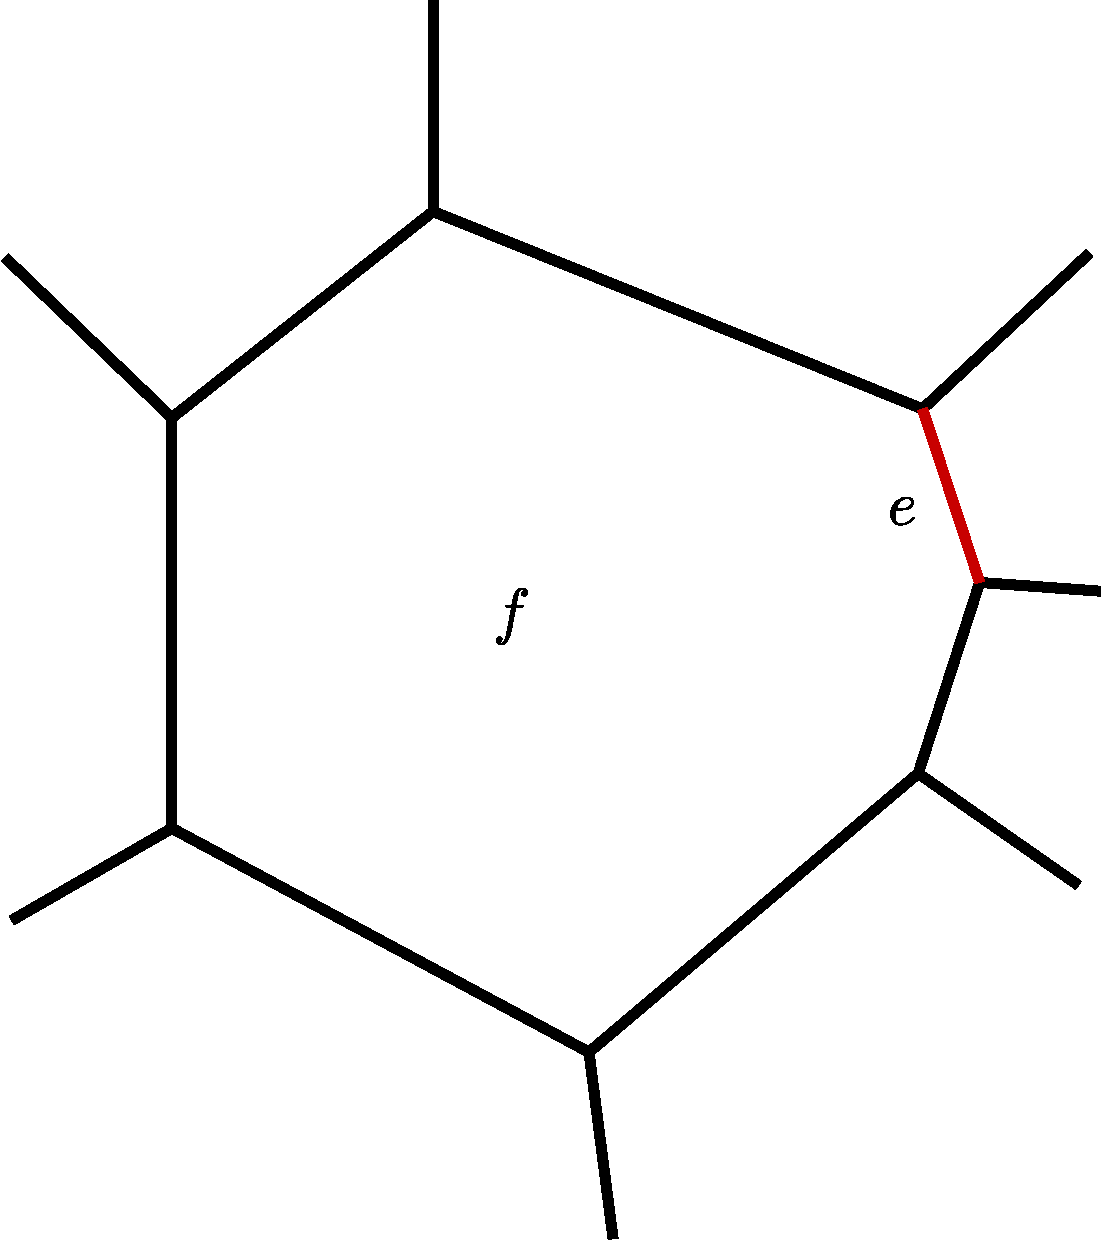
\includegraphics[scale=0.25]{lemma_edge_contraction_fig_1_crop}
	\hspace*{0.4in}
	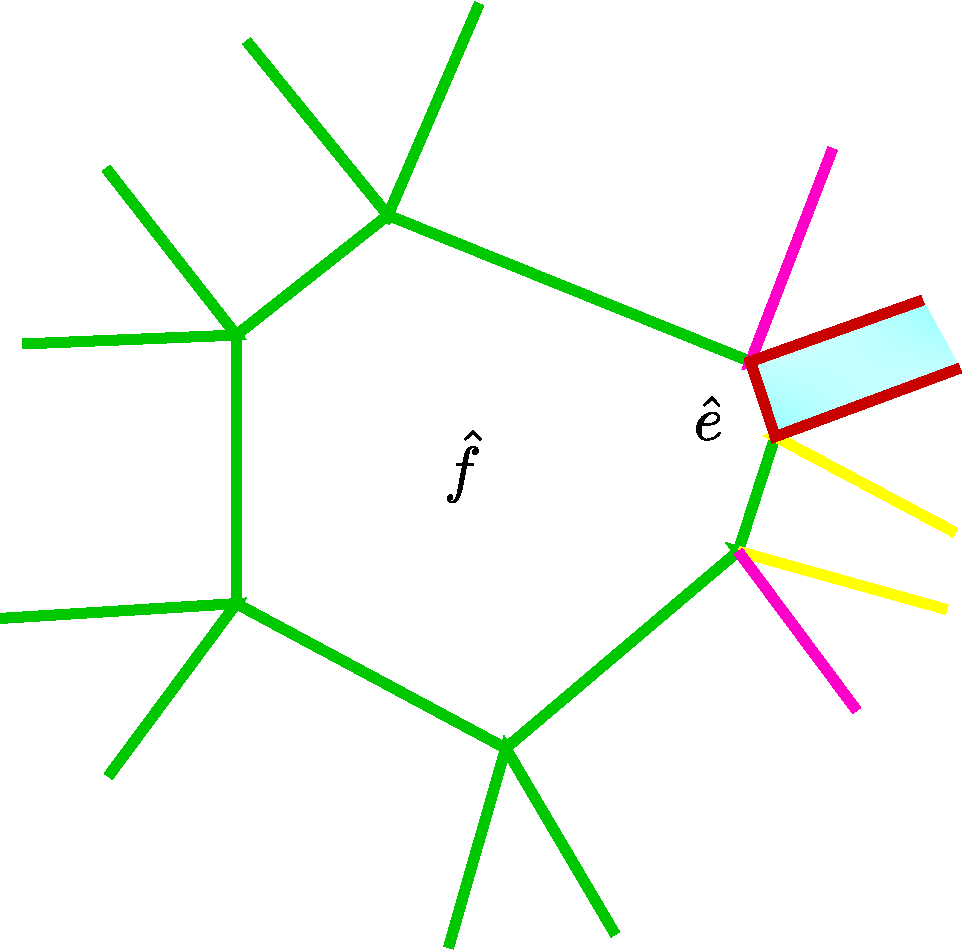
\includegraphics[scale=0.35]{lemma_edge_contraction_fig_2_crop}
        \vspace*{0.1in}\\
	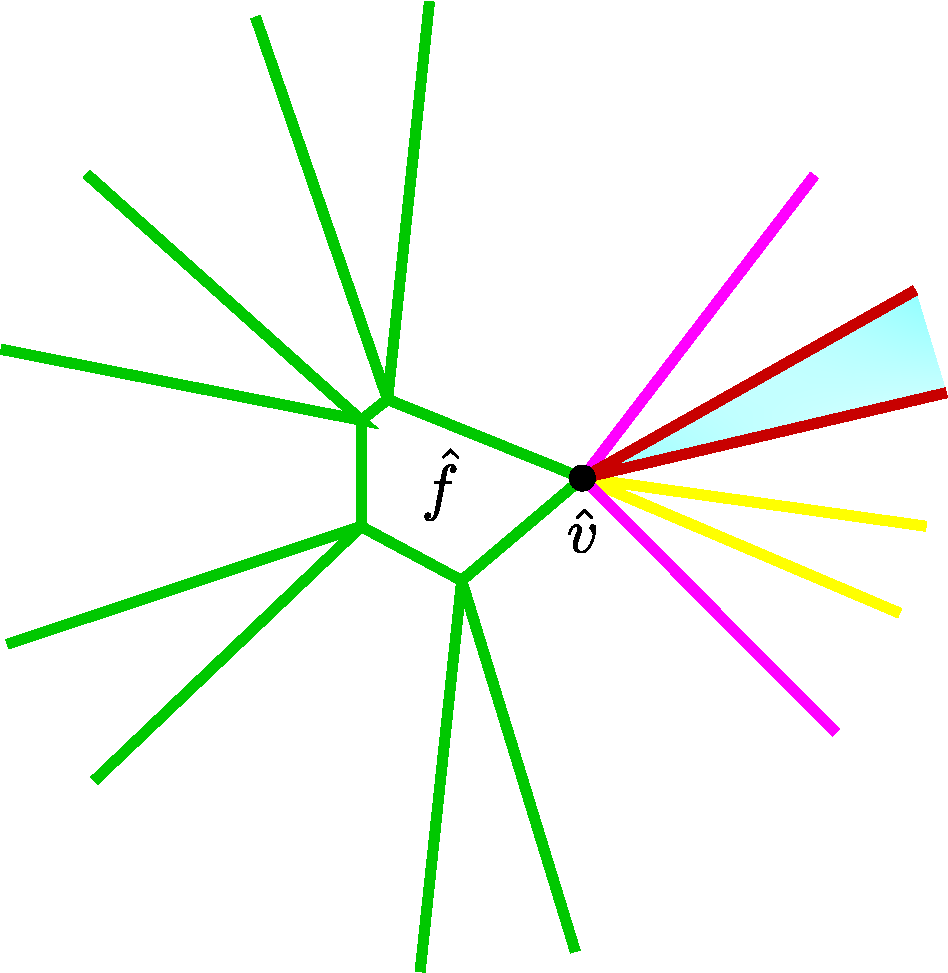
\includegraphics[scale=0.35]{lemma_edge_contraction_fig_3_crop}
	\hspace*{0.4in}
	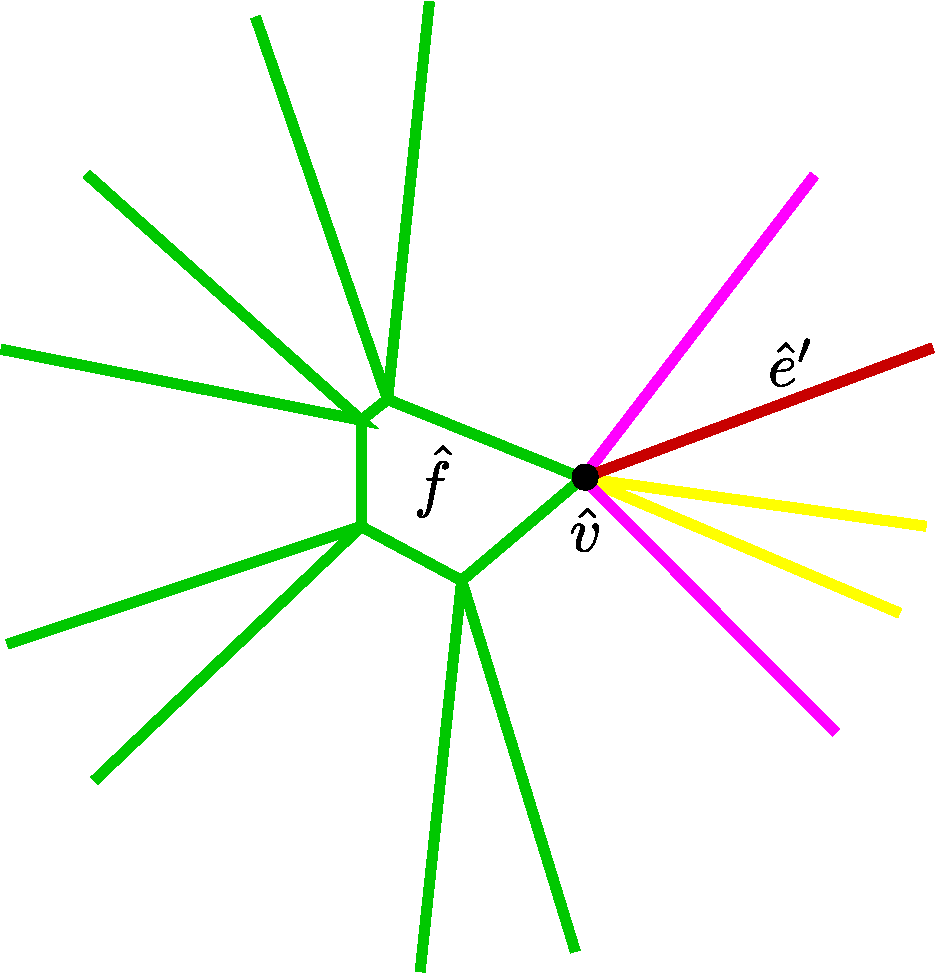
\includegraphics[scale=0.35]{lemma_edge_contraction_fig_4_crop}
	\caption{\label{fig:lemmaedgecontraction}
		$f$ is a polygon in $K$ (top left).
		Euler transformation of $K$ into $\hK$ (top right), where $\hf$ is the Class $1$ polygon corresponding to $f$, and $\hf_e$ (blue) is the Class $2$ polygon corresponding to edge $e$.
		Combinatorial changes are allowed in $\hK$ in the bottom left figure, and edge $\he$ of $\hf$ is collapsed to a point $\hv$ where $\hf_e$ (blue) is a triangle.
		As $\he \in \hf_e$ is collapsed to a point, the degree of $\hv$ in the $1$-skeleton of $\hK$ is $2(2) + 4 = 8$.
		In the version of $\hK$ shown in the bottom right figure, an edge of $\hf_e$ shared with some Class $1$ polygon other than $\hf$ is also collapsed to a point.
		Here, $\hf_e$ is collapsed to an edge $\he'$ (red) and the degree of $\hv$ in the $1$-skeleton of $\hK$ is $2(2) + 4 - 1= 7$.
	}
\end{figure}

\begin{figure}[hbp!] 
  \centering
  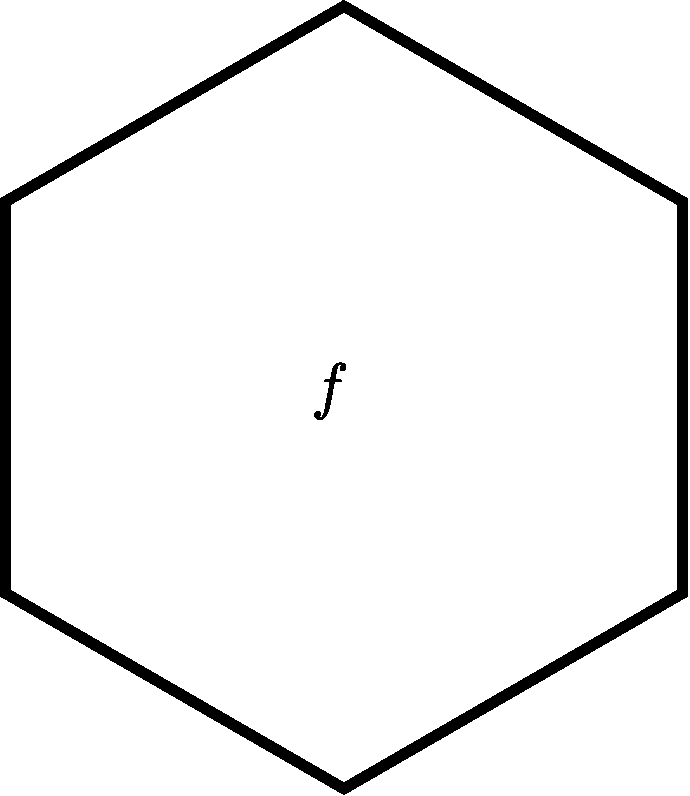
\includegraphics[scale=0.3]{2_cell_partition_fig_1_crop}
  \hspace*{0.25in}
  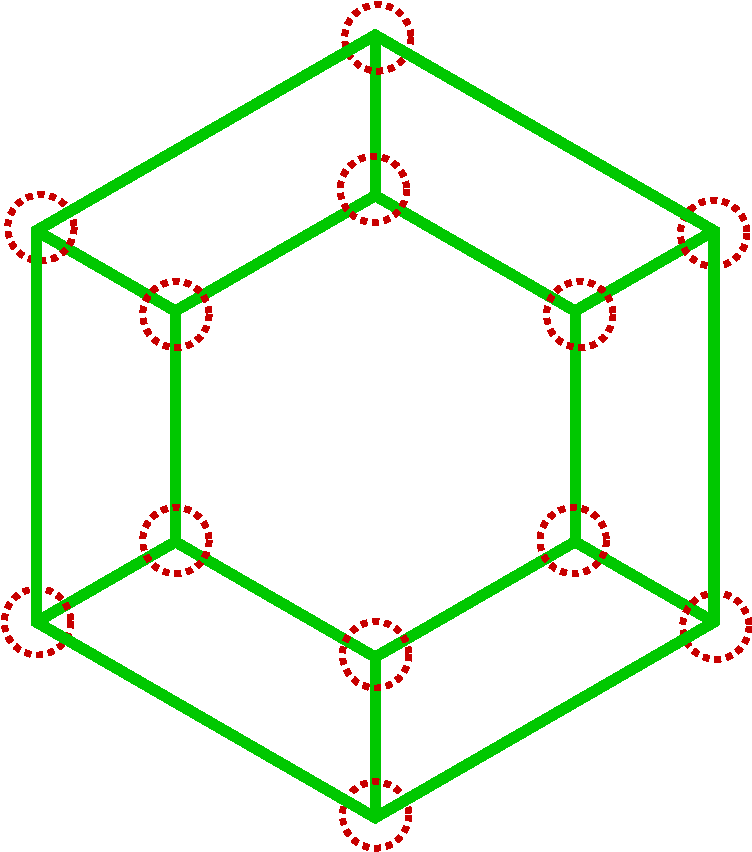
\includegraphics[scale=0.3]{2_cell_partition_fig_2_crop}
  \hspace*{0.25in}
  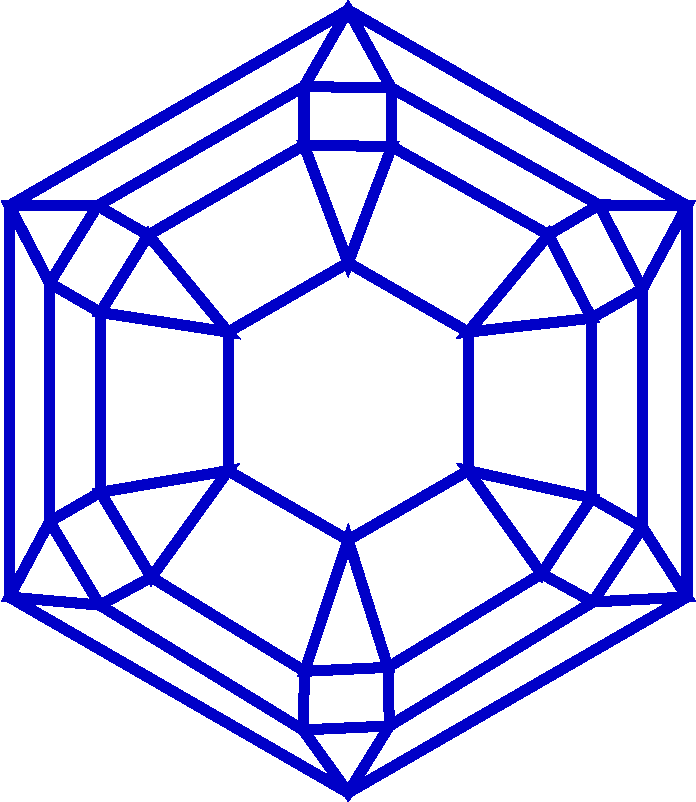
\includegraphics[scale=0.3]{2_cell_partition_fig_3_crop}
  \caption{\label{fig:2cellpartition}
    $\hK$ consisting of a single polygon $f$ (left) and its Euler transformation $\hK$ in green (middle).
    Vertices circled in red have odd degrees.
    The complex in blue (right) is the Euler transformation of $\hK$, and its $1$-skeleton is Euler.}
\end{figure}

\begin{lem}
  \label{lem:combinatorialdegree}
  Let $\hv$ is a vertex in a Class $1$ polygon $\hf$ of $\hK$ created after collapsing $\pi$ adjacent edges in $\hf$, where $\hf$ is allowed to have combinatorial changes.
  Let $\hf_e$ is some Class $2$ polygon that contains one of these collapsed adjacent edges.
  If no $\hf_e$ is collapsed into an edge, then degree of $\hv$ is $~2\pi + 4~$ else $~2\pi + 4 - m~$ where $m$ is the number of polygons similar to $\hf_e$ collapsed into an edge. 
\end{lem}
\begin{proof}
  Since a polygon $\hf$ is allowed to have combinatorial changes in $\hK$, it will change degree of vertices in $\hf$.
  $\pi$ adjacent edges in $\hf$ have $\pi + 1$ vertices.
  Each end vertex of the path created by $\pi$ adjacent edges adds $3$ edges to $\hv$, and each interior vertex of the path adds $2$ edges to $\hv$ as shown in \cref{fig:lemmaedgecontraction}.
  This implies $\hv$ has degree $2(\pi -1) + 3 + 3 = 2\pi + 4$ and $1$-skeleton of $\hK$ is still Euler.
  If $m > 0$ Class $2$ polygons sharing one of these adjacent edges are allowed to collapse into an edge, then $2$ edges sharing $\hv$ of each collapsed Class $2$ polygon is replaced by one edge.
  Also, $m \leq \pi$ since each distinct edge in any Class $1$ polygon is shared by a unique Class $2$ polygon in the Euler transformation.
  This implies $\hv$ has degree $2\pi + 4 -2m + m = 2\pi + 4 - m$ and $1$-skeleton of $\hK$ is Euler depending upon $m$ is even or odd, as shown in Figure \ref{fig:lemmaedgecontraction}.
\end{proof}
%\clearpage


If combinatorial changes are allowed during Euler transformation, then for any odd degree vertices created, we should apply Euler transformation to a local complex.
In the following result, we use the generalized Euler transformation to address the issue of odd degree vertices that may be created by combinatorial changes in $\hK$.
%\newline


\begin{lem}
  \label{lem:localeulertransformation}
  Suppose $\hf_e$ in $\hK$ is collapsed to an edge $\he$, since combinatorial changes are allowed in $\hK$.
  Suppose $\hk$ is a sub $2$-complex of $\hK$ consisting of Class $3$ polygons sharing any edge $\he$ in $\hK$,
  and let $\hk_j$ be a single component contained in $\hk$, since $\hk$ can have multiple components.
  Suppose $\hk_j = \cup \tilde{k}_i$, where $\tilde{k}_i$ is sub $2$-complex in $\hk_j, \hK$, and let $\tilde{k}_i, \tilde {k}_j$ do not share any edge in $\hK$, if $i \neq j$.
  If $\check{k}_i$ is the generalized Euler transformation of $\tilde{k}_i$ and $\bar{k}_j = \cup \check{k}_i$ is single component in $\bar{k}$, then the $1$-skeleton of $(\hK \smallsetminus \hk) \cup \bar{k}$ is Euler.  	
\end{lem}



\begin{figure}[htp!] 
  %\centering
  \begin{subfigure}[t]{2.5in}
    \centering
    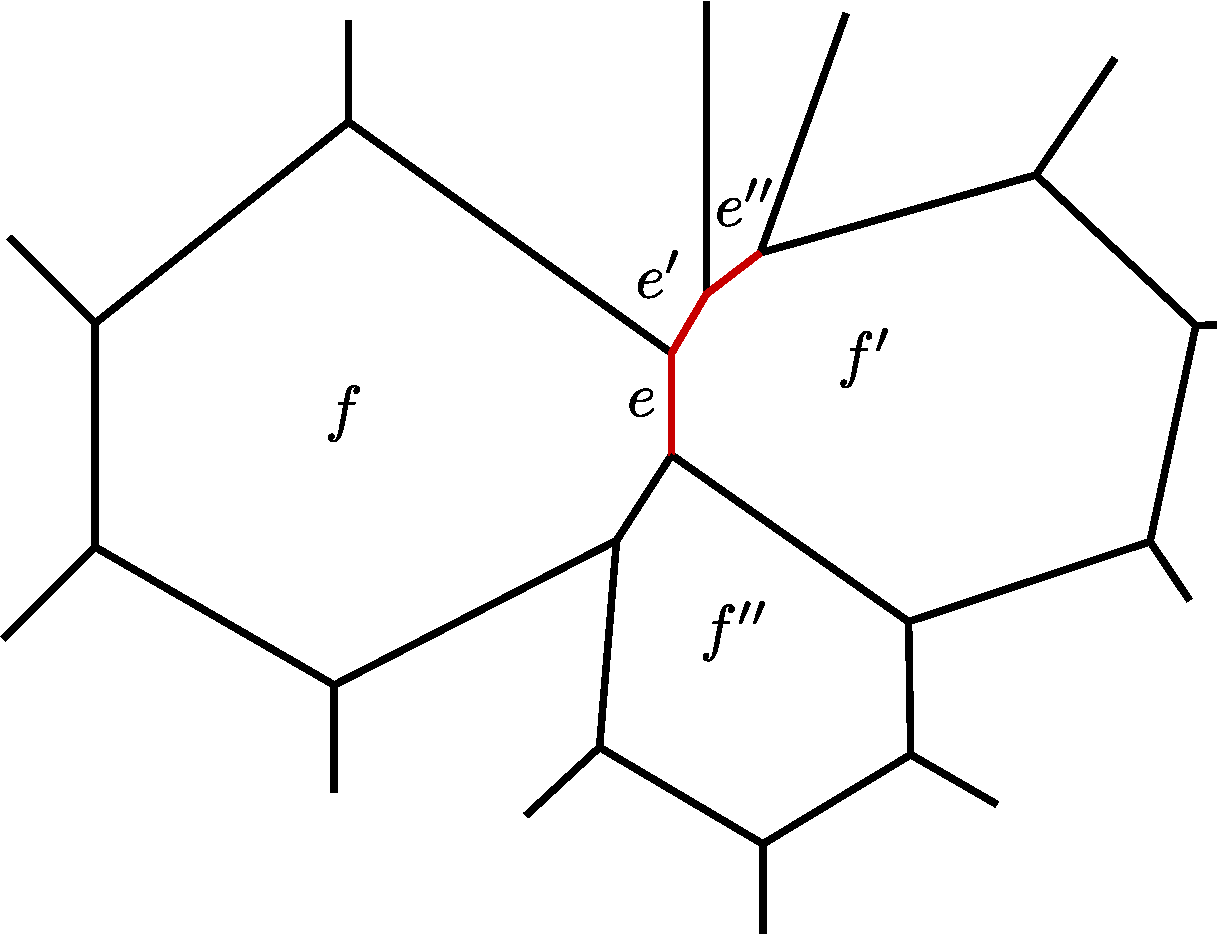
\includegraphics[scale=0.38]{lemma_local_euler_transformation_fig_1_crop}
    \caption{\label{fig:lemmalocaleulertransformationa}}
  \end{subfigure}
  \hspace*{0.8in}
  \begin{subfigure}[t]{2.5in}
    \centering
    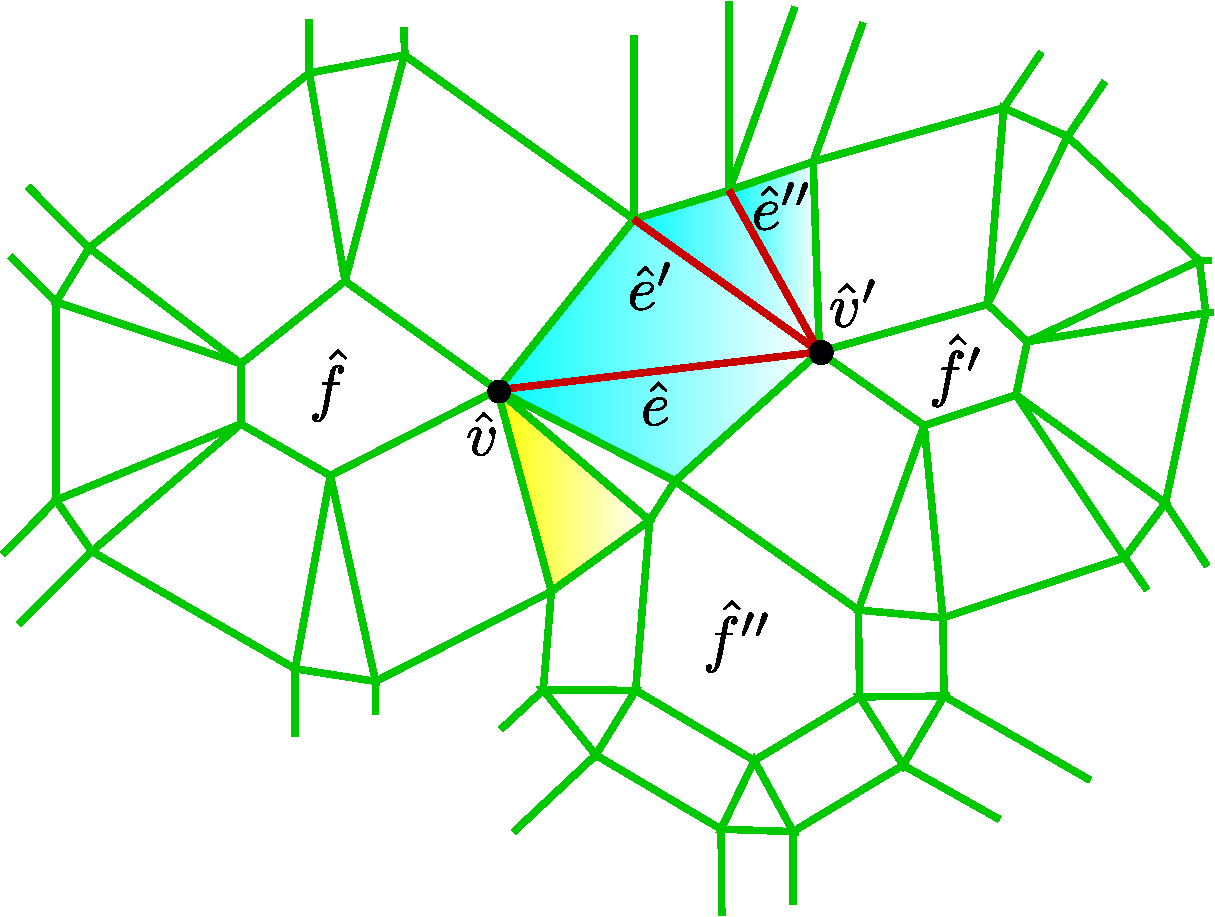
\includegraphics[scale=0.38]{lemma_local_euler_transformation_fig_2_crop}
    \caption{\label{fig:lemmalocaleulertransformationb}}
  \end{subfigure}
  \vspace*{0.3in}\\	
  \begin{subfigure}[t]{2.5in}
    \centering
    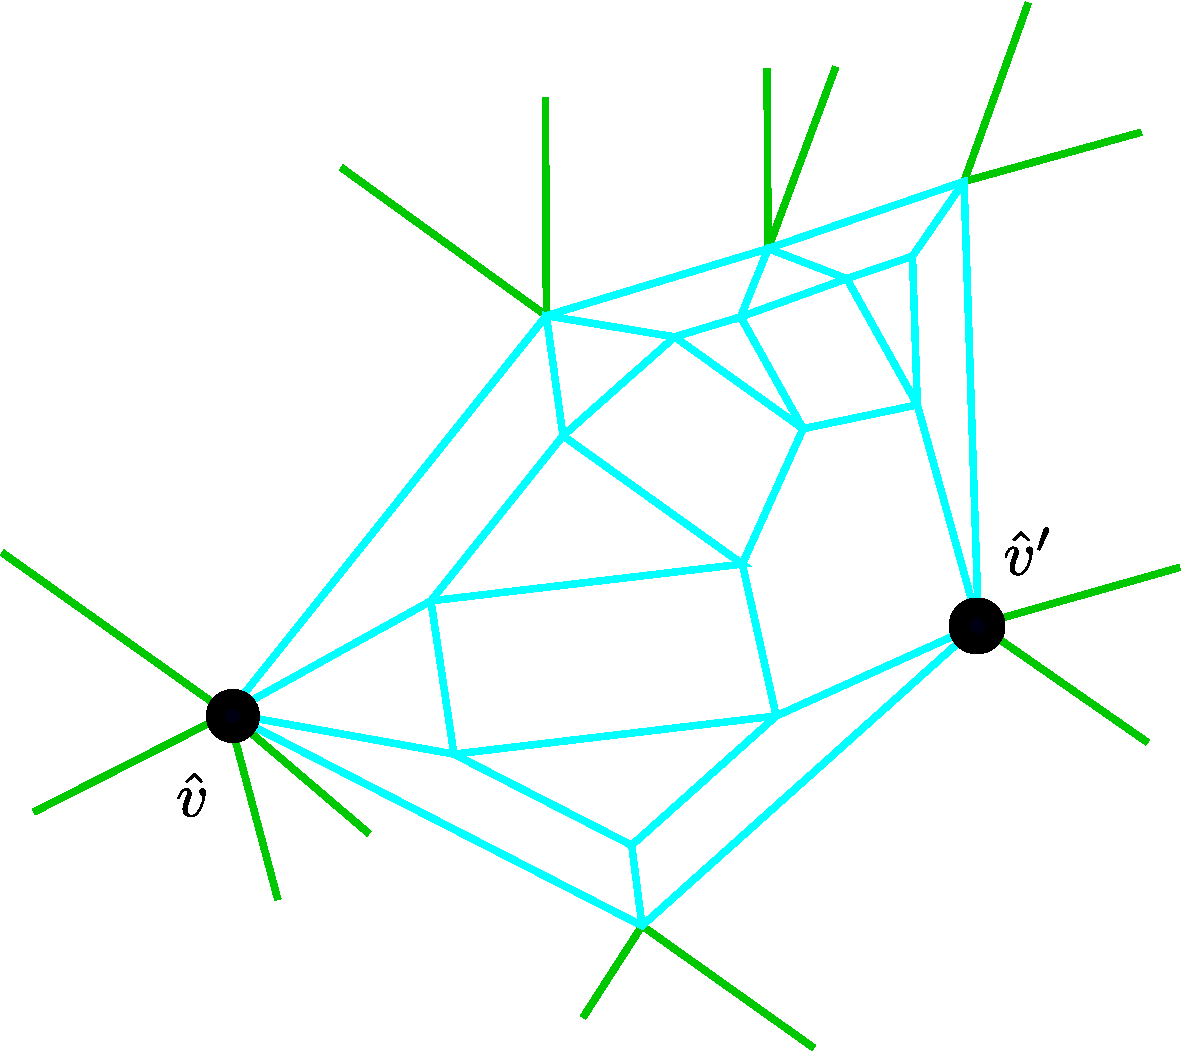
\includegraphics[scale=0.38]{lemma_local_euler_transformation_fig_3_crop}
    \caption{\label{fig:lemmalocaleulertransformationc}}
  \end{subfigure}
  \hspace*{0.8in}		
  \begin{subfigure}[t]{2.5in}
    \centering
    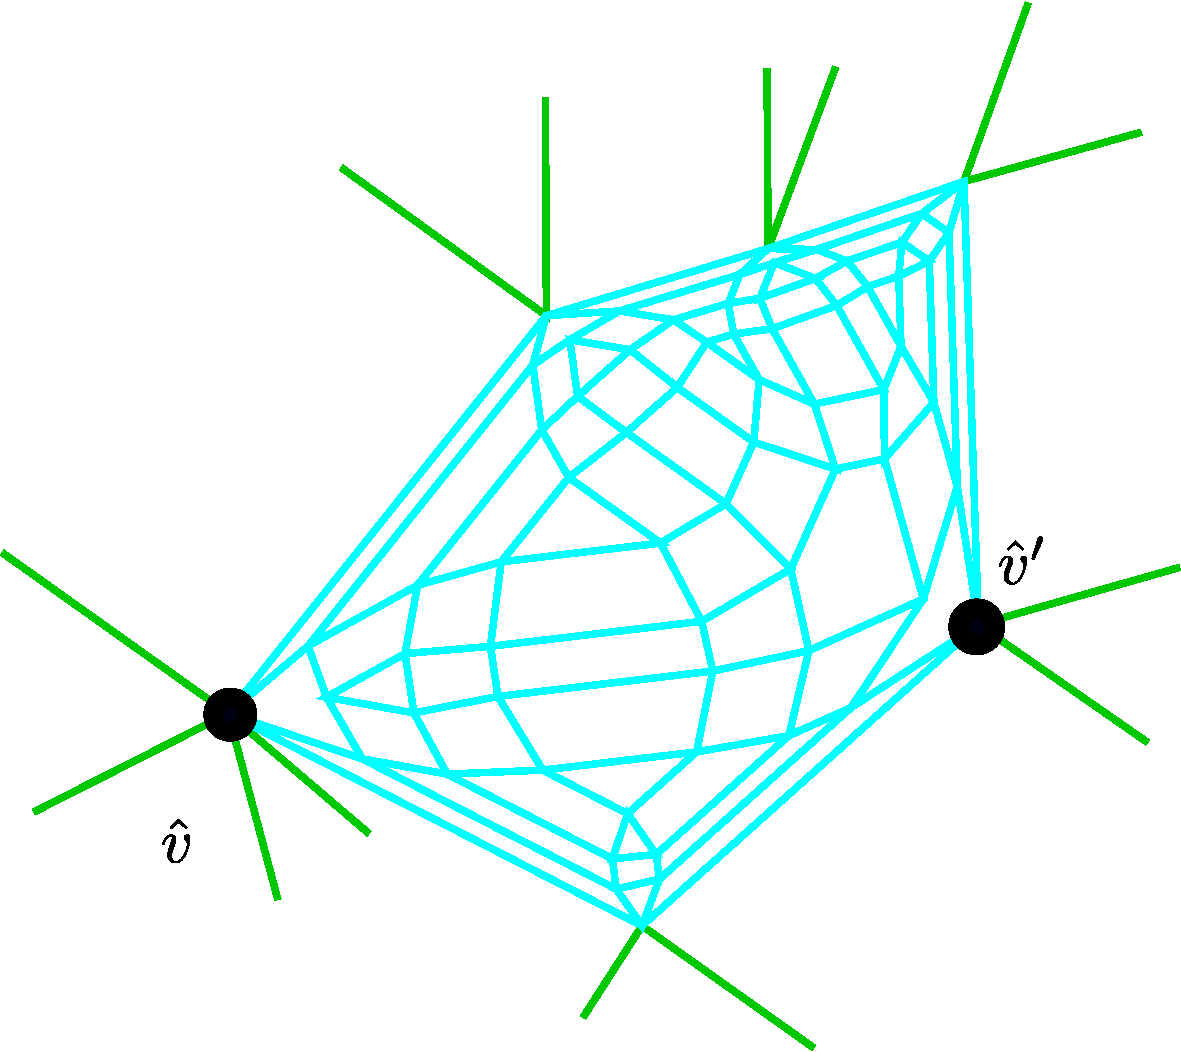
\includegraphics[scale=0.38]{lemma_local_euler_transformation_fig_4_crop}
    \caption{\label{fig:lemmalocaleulertransformationd}}
  \end{subfigure}
  \caption{  \label{fig:lemmalocaleulertransformation}
    (a) $f, f', f''$ are polygons in $2$-complex $K$.
    (b) $2$-complex $\hK$ after Euler transformation with combinatorial changes to some polygons in $\hK$. Class $2$ polygons $\hf_e,\hf_{e'}, \hf_{e''}$ corresponding to $e, e', e''$ in $K$ are collapsed into edges $\he, \he', \he''$.
    Sub $2$-complex $\tilde{k}_i$ (in blue) of some $\hk_j$ in $\hK$ consists of Class $3$ polygons sharing edges $\he, \he', \he''$ in the $1$-skeleton of $\tilde{k}_i$, and has vertices $\hv, \hv'$ with odd degree $7$.
    The number of edges (green) at each vertex of $\tilde{k}_i$ not in $\tilde{k}_i$ are even, $\hv$ has $1$ Class $3$ polygon(yellow) not contained in $\tilde{k}_i$. (c),(d) shows generalized Euler transformation of $\tilde{k}_i$. (d) $\check{k}_i$(blue) is generalized Euler transformation of $\tilde{k}_i$ and $\hv, \hv'$ including other vertices of $\check{k}_i$ has even degree in $1$-skeleton of $\hK \smallsetminus \tilde{k}_i \cup \check{k}_i$.
  }
\end{figure}

\begin{proof}
  Since combinatorial changes are allowed in $\hK$, let $\hv$ be a vertex in $\hk_j$ created after $\pi$ adjacent edges of $\hf$ are collapsed to a vertex.
  $\hk_j$ is single component in $\hk$, and only Class $3$ polygons share an edge with any collapsed Class $2$ polygons $\hf_e$ is in $\hk_j$.
  Hence $\hv$ can be shared by some Class $3$ polygon not in $\hk_j$.
  If any Class $3$ polygon sharing $\hv$ is not contained in $\hk_j$, this Class $3$ polygon does not share an edge with any Class $2$ polygon.
  Hence such cells do not belong to any component $\hk_j$ in $\hk$.
  Since Class $1$ polygons are edge disjoint from any Class $3$ polygons, and there are some Class $3$ polygons and $1$ Class $1$ polygon ($\hf$) sharing vertex $\hv$ in $\hK$ but not contained in $\hk_j$, we get that $\hv$ is shared by an even number of additional edges not in $\hk_j$.
  Since Class $1$ and Class $3$ polygons are edge disjoint in $\hK$, then any vertex($\hv'$) in some Class $3$ polygon in $\hk_j$ not similar to $\hv$ has $2$ more edges, not in $\hk_j$ sharing $\hv'$.
  Hence all the vertices in $\hk_j$ have even number of additional edges in $\hK$ not contained in $\hk_j$ as shown in Figure \ref{fig:lemmalocaleulertransformation}.
  
  Let $\check{k}_i$ be the generalized Euler transformation of each sub $2$-complex $\tilde{k}_i \in \hk_j$.
  Then any vertex in $\hK \smallsetminus \hk \cup \bar{k}$ has an even number of edges connected to it, since each $\bar{k}_j = \cup \check{k}_i$ contributes even number of edges to any vertex shared by $\bar{k}_j$ and each vertex in $\hk$ has $2$ more edges not contained in $\hk$.
  Hence the $1$-skeleton of $(\hK \smallsetminus \hk) \cup \bar{k}$ is Euler. 
\end{proof}

Let vertex $\hv$ in the sub $2$-complex $\tilde{k}_i$ of single component $\hk_j$ in $\hk$ have odd  number of edges connected to it in $\tilde{k}_j$.
We apply generalized Euler transformation to any such sub $2$-complex $\tilde{k}_i$.
Then by Lemma \ref{lem:localeulertransformation}, the new $2$-complex is Euler.



\subsection{Euler Transformation with Topological Changes}\label{sec:eulertransformwithTopolog}
When a polygon $f$ in $K$ is split into multiple class-$1$ polygons in $\hat{K}$ after mitered offset, it is said to undergo a \emph{topological change} (see \cref{fig:topologychangelemma}). 
If polygons in the $2$-complex $K$ are concave, then their mitered offset could create topological changes.
Without loss of generality we assume the $2$-complex $K$ consists of polygons satisfying \cref{asmn:Kholesoutside}, and its polygons can be convex or concave (but are still homeomorphic to a $2$-ball by definition). %

\begin{figure}[ht!] 
	\centering
	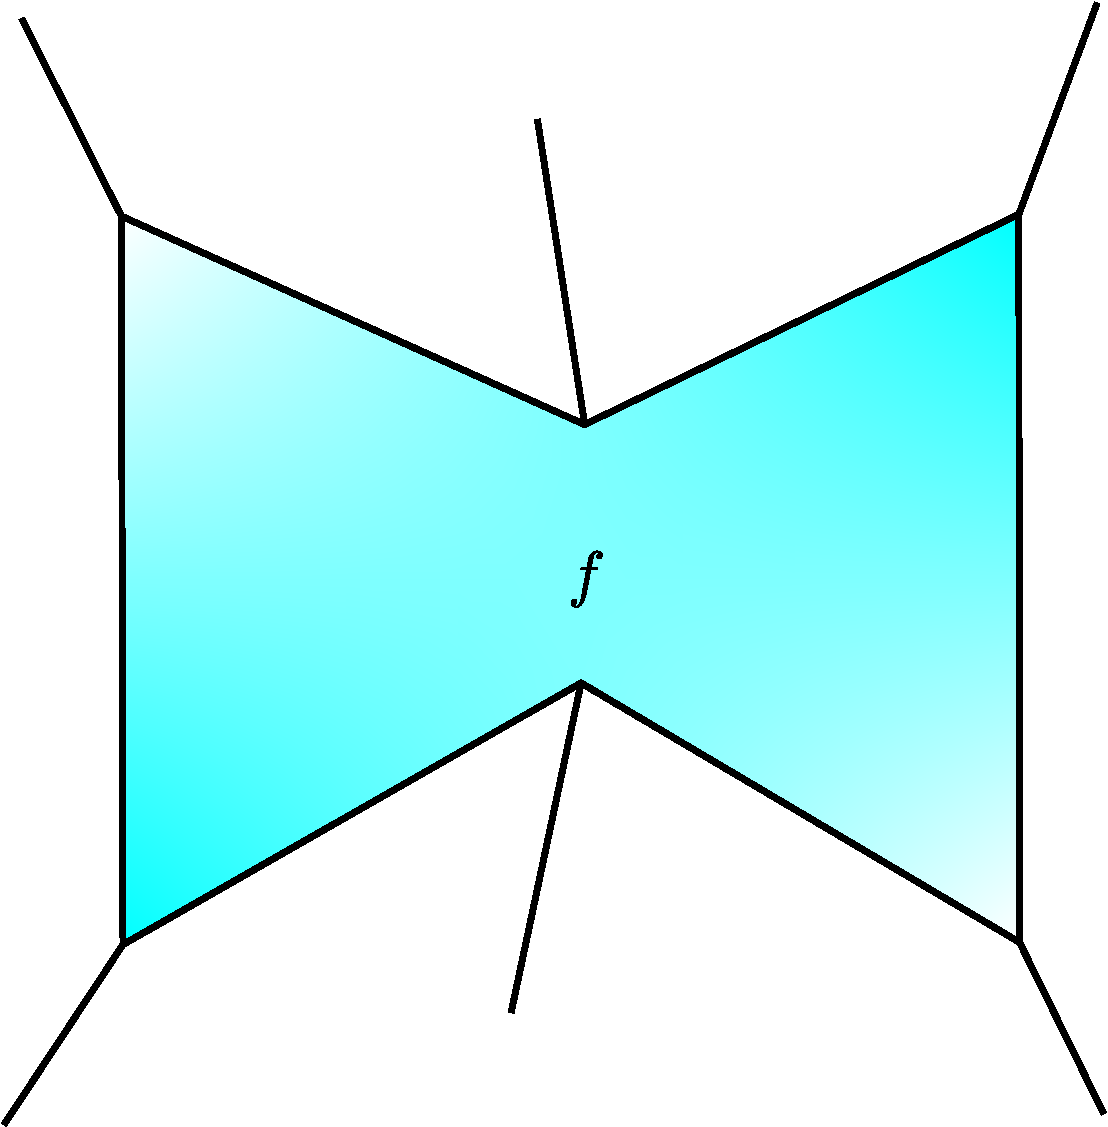
\includegraphics[scale=0.26]{topology_change_lemma_fig_0_crop}
	\quad
	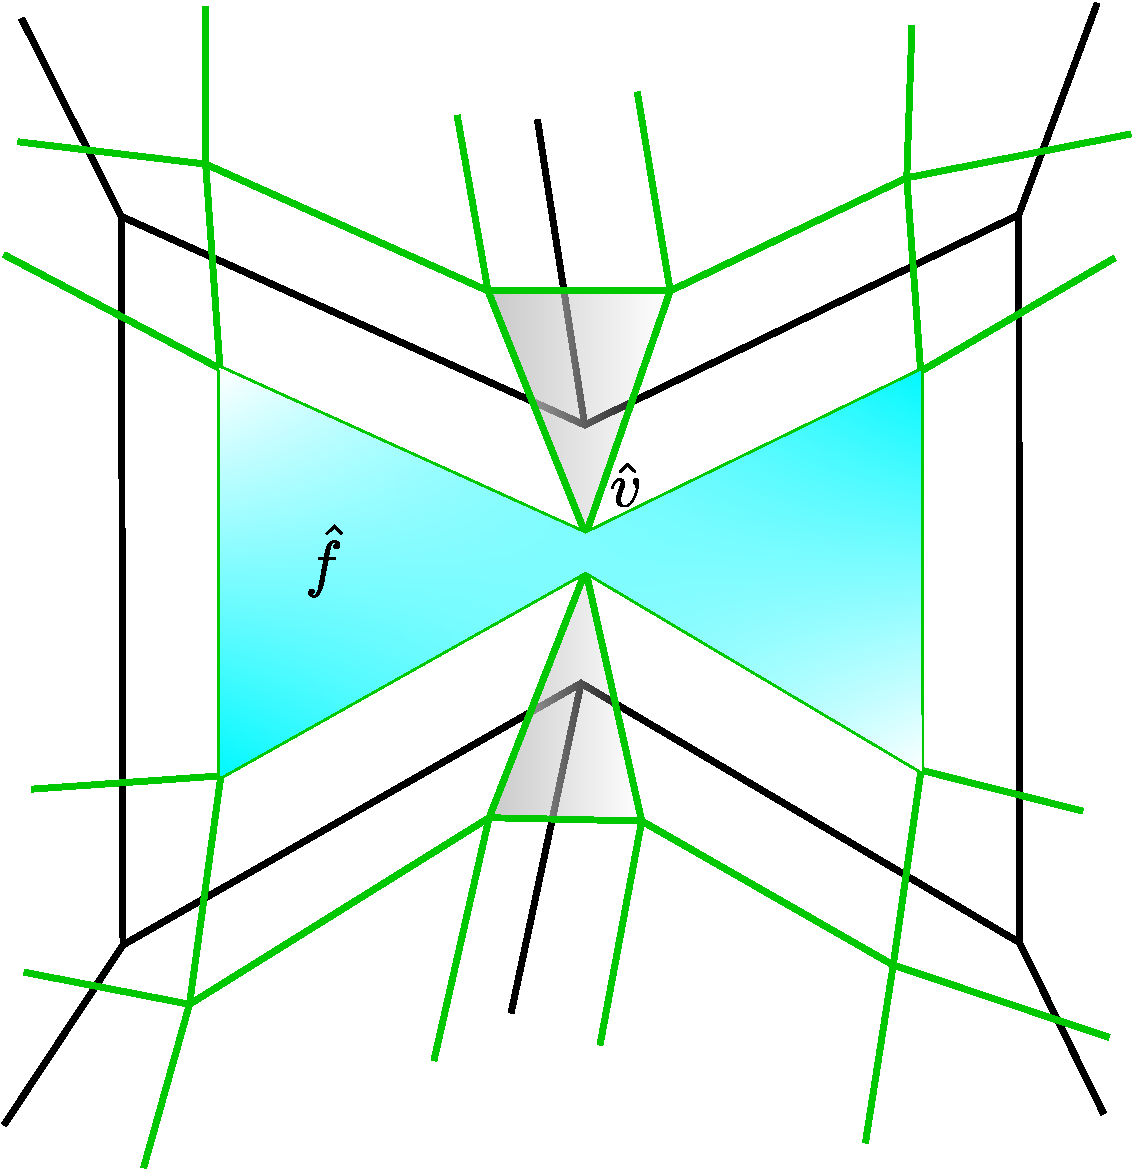
\includegraphics[scale=0.26]{topology_change_lemma_fig_1_crop}
	%\quad
        \vspace*{0.1in}\\
	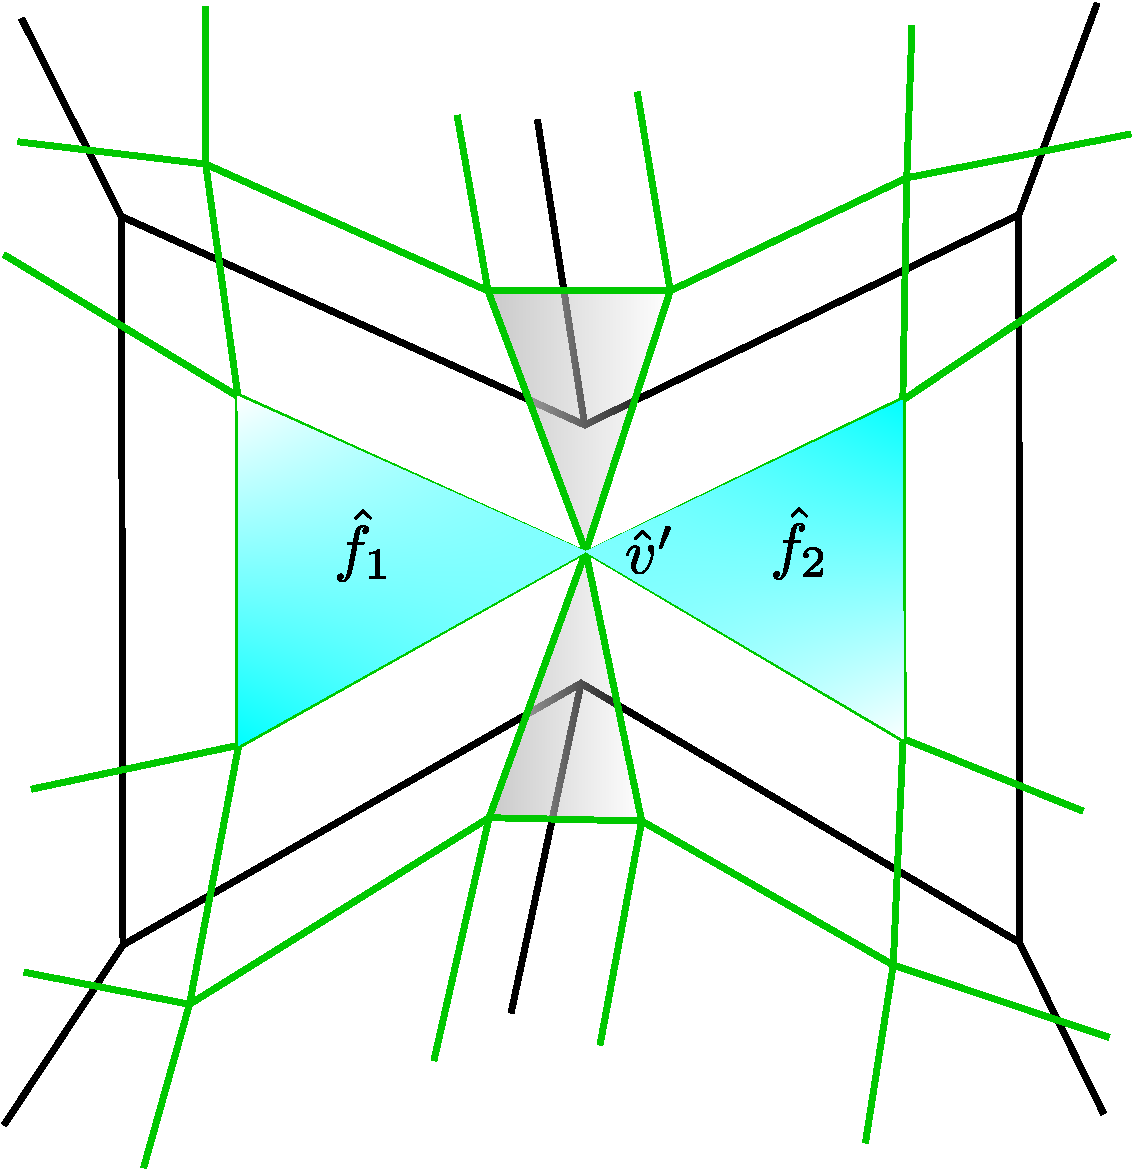
\includegraphics[scale=0.26]{topology_change_lemma_fig_2_crop}
	\quad
	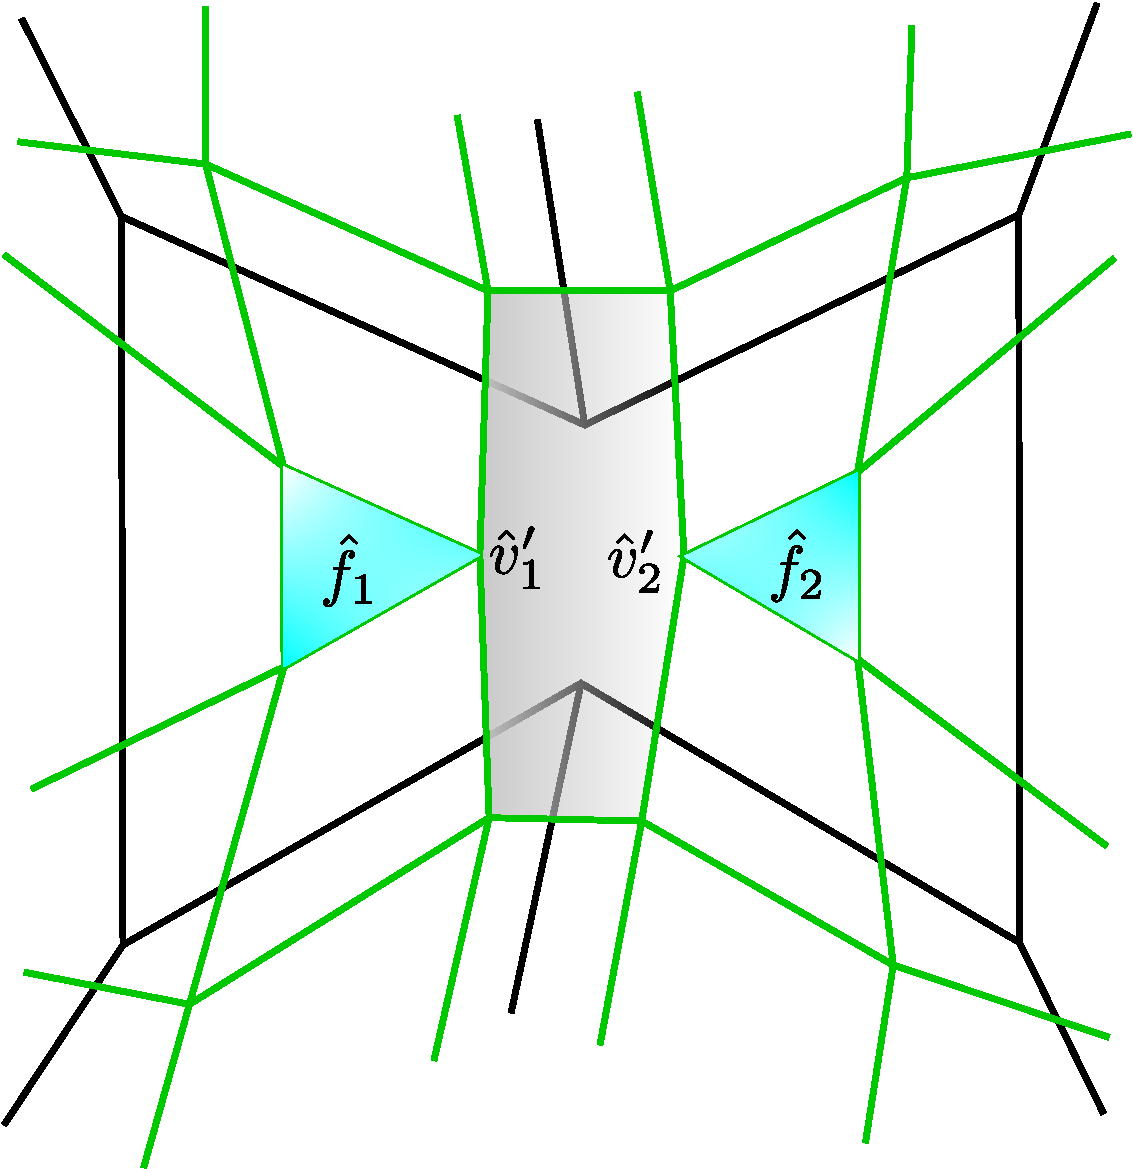
\includegraphics[scale=0.26]{topology_change_lemma_fig_3_crop}
	\caption{\label{fig:topologychangelemma}
          (Top left) Non-convex polygon $f$ (Blue) in $K$.
          (Top right) Polygon $\hf$ (blue) and Class \ref{2dETcls3} polygon (shaded black) in $\hK$.
          (Bottom left) $\hat{f}$ split into two polygons $\hat{f}_1, \hat{f}_2$(Blue) by joining two vertices of $\hat{f}$ to $\hat{v}'$. Since $\hat{f}_1, \hat{f}_2$ and class-3 polygons(Shaded black) at $\hat{v}'$ are edge-disjoint then $\hat{v}'$ has degree $8$ and $q=2$.
          (Bottom-right) $\hat{f}_1, \hat{f}_2$ are completely disjoint and $\hat{v}'$ split up into $\hat{v}'_1, \hat{v}'_2$ creating one polygon $F$(Shaded black), where $\hat{v}'_1, \hat{v}'_2$ has degree $4$. }
\end{figure}  

\begin{lem}
  Let the complex $\hat{K}$ be created by Euler transformation with some polygons undergoing only topological (no combinatorial) changes.
  Then the degree of vertices in $\hat{K}$ is even.
  Furthermore, if $K$ is connected, then so is $\hat{K}$. 
\end{lem}
\begin{proof}
	%Without loss of generality consider cells as shown in Figure \ref{fig:topologychangelemma} of initial complex $K$ which satisfies input conditions. To create transformed complex $\hat{K}$ we applies Euler transformation with some offset distance. Since $f$ is concave, then with increase in offset distance first $\hat{v}, \hat{v}'$ will join and replace by $\hat{v}''$ and second $\hat{v}''$ will split into two vertices $\hat{v}''', \hat{v}''''$ causing topological changes. Accordingly with increase in offset distance, class-$1$ polygon $\hat{f}$ created is first replaced by two polygons $\hat{f}', \hat{f}''$, where $\hat{f}', \hat{f}''$ are disjoint. Total number of edges in $\hat{f}$, and $\hat{f}'\cup \hat{f}''$ are still the same, i.e there are no combinatorial changes. $\hat{v}''$ has degree $8$ since it is contained in $\hat{f}', \hat{f}'', \hat{f}_v, \hat{f}_{v'}$ edge disjoint polygons in $\hat{K}$ as shown in the Figure. $\hat{v}'''$ is connected to $2$ edges($\hat{e}' , \hat{e}''$) contained in $\hat{f}'$ and two other edges contained in $\hat{f}_{e}$, $\hat{f}_{e''}$ $\implies$ $\hat{v}'''$ has degree 4. Similarly we can show  $\hat{v}''''$ has degree 4.	
	%With increase in offset distance, first class-$2$ polygons $\hat{f}_v, \hat{f}_{v'}$ are joined  and then replaced by polygon $f_{vv'}$, around vertices $v, v'$. 
  When there are no topological changes, any vertex $\hv$ in polygon $\hf$ is shared by edge-disjoint Class \ref{2dETcls1} and \ref{2dETcls3} polygons in $\hK$. 
  Let us allow topological changes to $\hf$.
  There are two possible cases.
  In the first case, $\hf$ splits into multiple polygons at vertex $\hat{v}'$ by joining two or more vertices in $\hf$ due to mitered offset.
  Then $\hat{v}'$ is still shared by edge-disjoint Class \ref{2dETcls3} polygons as shown in \cref{fig:topologychangelemma}.
  In the second case, if we further increase the offset distance then $\hv'$ will split into $q$ new vertices ($\hat{v}'_1, \dots, \hat{v}'_q$), where $q$ is the number of Class \ref{2dETcls3} polygons sharing $\hat{v}'$ in the first case.
  It will also join $q$ Class \ref{2dETcls3} polygons sharing vertex $\hat{v}'$ into one polygon ($F$) as shown in \cref{fig:topologychangelemma}.
  Then any $\hat{v}_i'$ is shared by edge disjoint $F$ and class-$1$ polygons.
  Hence degree of vertices in $\hat{K}$ is even. 	   
  There exists a path from any vertex of the split polygon ($\hat{f}_i$) to any other vertex of $\hat{f}_j$, and hence $\hat{K}$ is connected since we assume $K$ is connected.
\end{proof}
	%Topological change may impact total euclidean length of edges in $\hat{K}$, but total number of edges will remain same before and after topological change in $\hat{K}$.	
If $q$ vertices are joined to create $\hat{v}'$ in $\hat{f}$ of $\hat{K}$ with increase in offset distance, then number of vertices $V' = V - q + 1$ and number of faces $F' = F + q -1 $ in $\hK$.
If we further increase the offset distance, $\hat{v}'$ will split into $q$ new vertices.
Then the number of vertices $V'' = V' - 1 + q = V$ and number of faces $F'' = F$, where $V$ and $F$ are original numbers of vertices and faces in $\hK$.
Note that the Euler characteristic and number of edges in $\hK$ remain the same after only topological changes in any class-$1$ polygon $\hat{f}$.  
	
We have discussed the cases when only combinatorial or only topological changes occur after transformation.
But if both \textit{combinatorial and topological changes} occur after transformation, then odd degree vertices are created due to combinatorial changes as shown in \cref{fig:combinatotopologychange}.
In this case, we can apply local Euler transformation to some subcomplex of $\hat{K}$, and then by \cref{lem:localeulertransformation} the $1$-skeleton of $\hat{K}$ is again Euler. 
	    
\begin{figure}[ht!] 
	\centering
	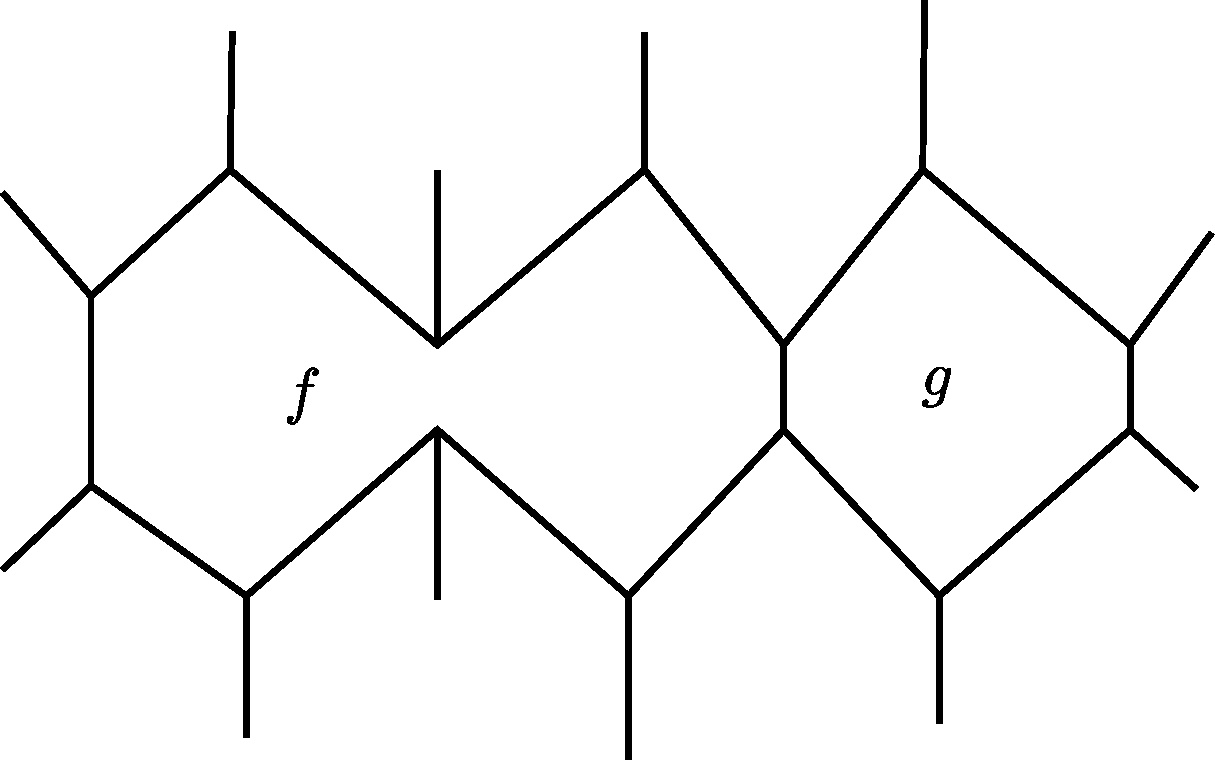
\includegraphics[scale=0.35]{input_example_3_crop}
	\quad
	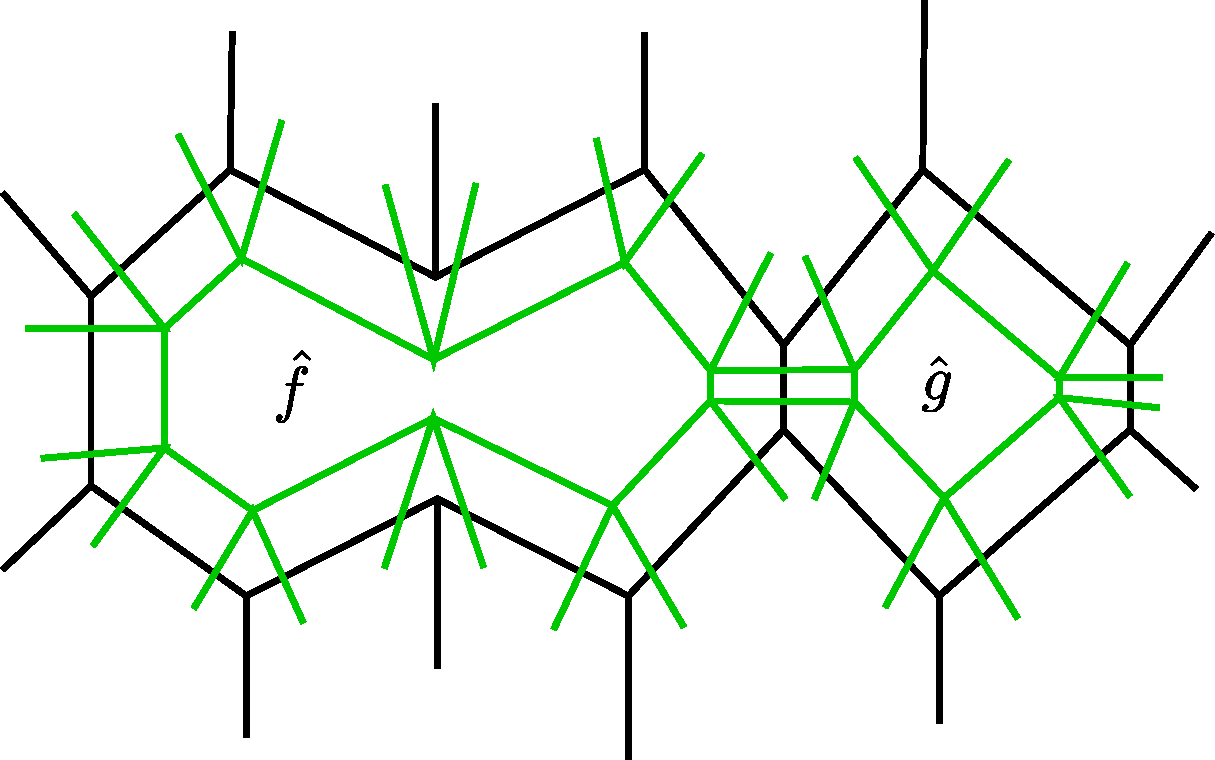
\includegraphics[scale=0.35]{euler_transformation_example_3_crop}
	%\quad
	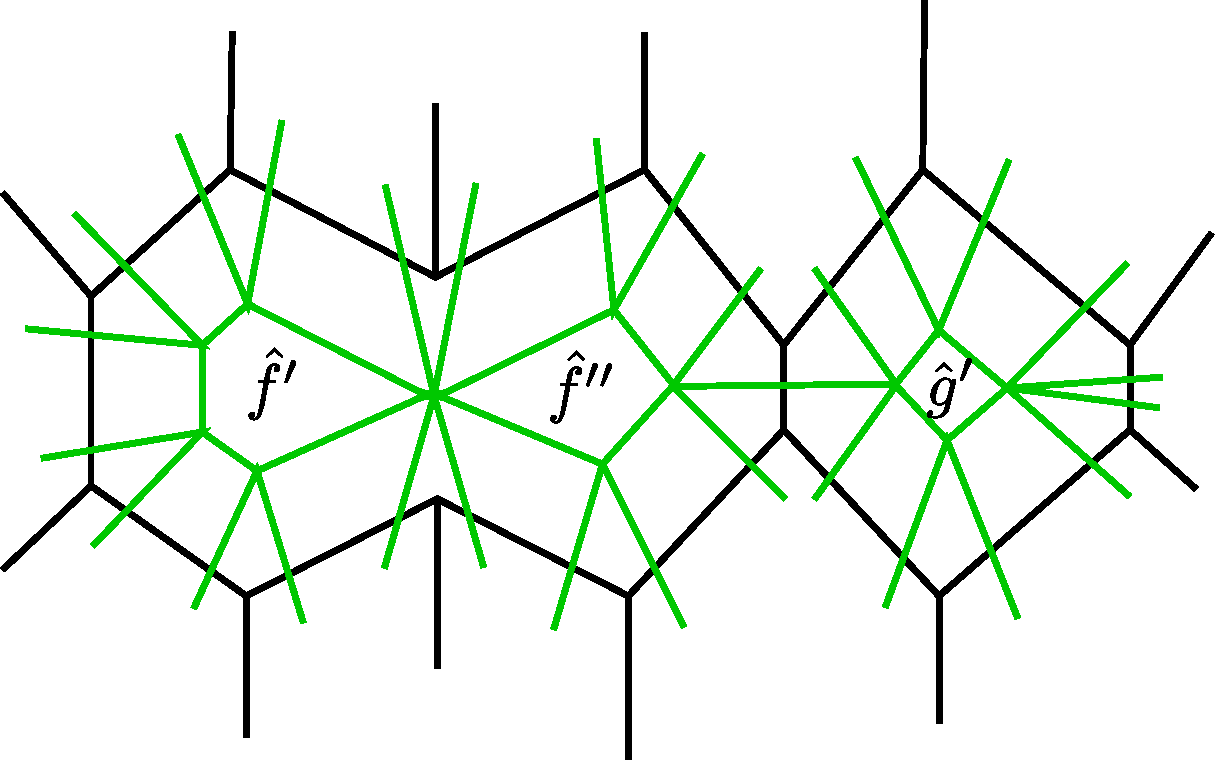
\includegraphics[scale=0.35]{euler_transformation_example_3_combinatorial_topological_change_crop}
	\caption{\label{fig:combinatotopologychange} $f, g$ are $2$, polygons in $K$ and $\hat{f}$, $\hat{g}$ are $2$ polygons in $\hK$. Second Figure shows no combinatorial and topological changes where as in Third Figure polygon $\hat{f}$ splits into $2$ polygons $\hat{f}', \hat{f}''$ with  both combinatorial and topological changes.}
\end{figure}

\section{Tool Path Algorithm}\label{sec:toolpathalgo}
Since $\tG$, the $1$-skeleton of $\tK$, is Euler, we can construct a tool path that consists only of the print path, i.e., all edges with none of them repeated.
In general, such a tour can cross over itself at a vertex, creating a special case of material collision termed \textit{crossover}.  
%can only be avoided with a travel path at the intersection.
We present a tool path algorithm that chooses the subcycles in an Eulerian tour of $\tG$ carefully so as to avoid all crossovers.
First we construct a circuit tree that represents $\tG$, with the vertices of the tree representing edge-disjoint circuits in $\tG$.
Second, we add edge traversal restrictions in order to avoid crossovers in the tool path, which is described by specifying a traversal order of the circuit tree. %except some boundary edges of $\tK$ where we can have travel paths if cells are too thin to prevent \textit{material collision} (see Figure \ref{fig:matcol})  and avoid print path \textit{crossover}.
%Since tool path mainly consists of print path it will improve quality of print, reduce print time.  
\subsection{Circuit Tree}

\begin{algorithm}[htp!] 
	\caption{CircuitTree}
	\label{alg:circuittree}
	\begin{algorithmic}[1]
		\State Unmark all the edges in $\tK$
		\State CircuitList =  FindBoundaryCircuits$(\tK$, $\emptyset)$
		\Comment{\textit{Initial } CircuitList \textit{contains one circuit} $C_{\rm Init}$}
		\State Mark all the edges in $\tK$ of $C_{\rm Init}$
		\State pred$(C_{\rm Init}) = \emptyset$ \Comment{\textit{Predecessor of} $C_0$ \textit{is empty}}
		\While{CircuitList $\neq \emptyset$}
		\State $C$ = CircuitList.pop$(0)$ 
		\State Circuits = FindBoundaryCircuits$(\tK$, $C)$ \Comment{\textit{Returns list of circuits}}
		\State CircuitList = CircuitList $\cup$ Circuits
		
		\While{Circuits $\neq \emptyset$}
		
		\State $C_s$ = Circuits.pop$(0)$ 
		\State pred$(C_s)$= $C$ \Comment{\textit{predecessor of $C_s$ is $C$}}
		\State Mark all the edges in $\tK$ of $C_s$
		
		\EndWhile
		  	
		\EndWhile
	\end{algorithmic}
\end{algorithm}

\begin{algorithm}[htp!] 
	\caption{FindBoundaryCircuits$(\tK,C_0)$}
	\label{alg:findboundarycircuit}
	\begin{algorithmic}[1]
	\State Find collection of edges $H$ based on $C_0$ \Comment{\textit{edges of cells intersecting $C_0$ not in $C_0$}}
	\State Circuits = \{\}	
     \While{$H \neq \emptyset $}
     
     %\State \textit{Circuit = \{\}}
     \State Find circuit $C$ using Modified Hierholzer's algorithm
     \State Remove all edges of $C$ from $H$
     \State Circuits = Circuits $\cup$ \{C\}
     
     \EndWhile			
	
	\State \Return Circuits
	\end{algorithmic}
	
\end{algorithm}

\begin{figure}[htp!] 
  \centering
  \vspace*{-0.1in}
	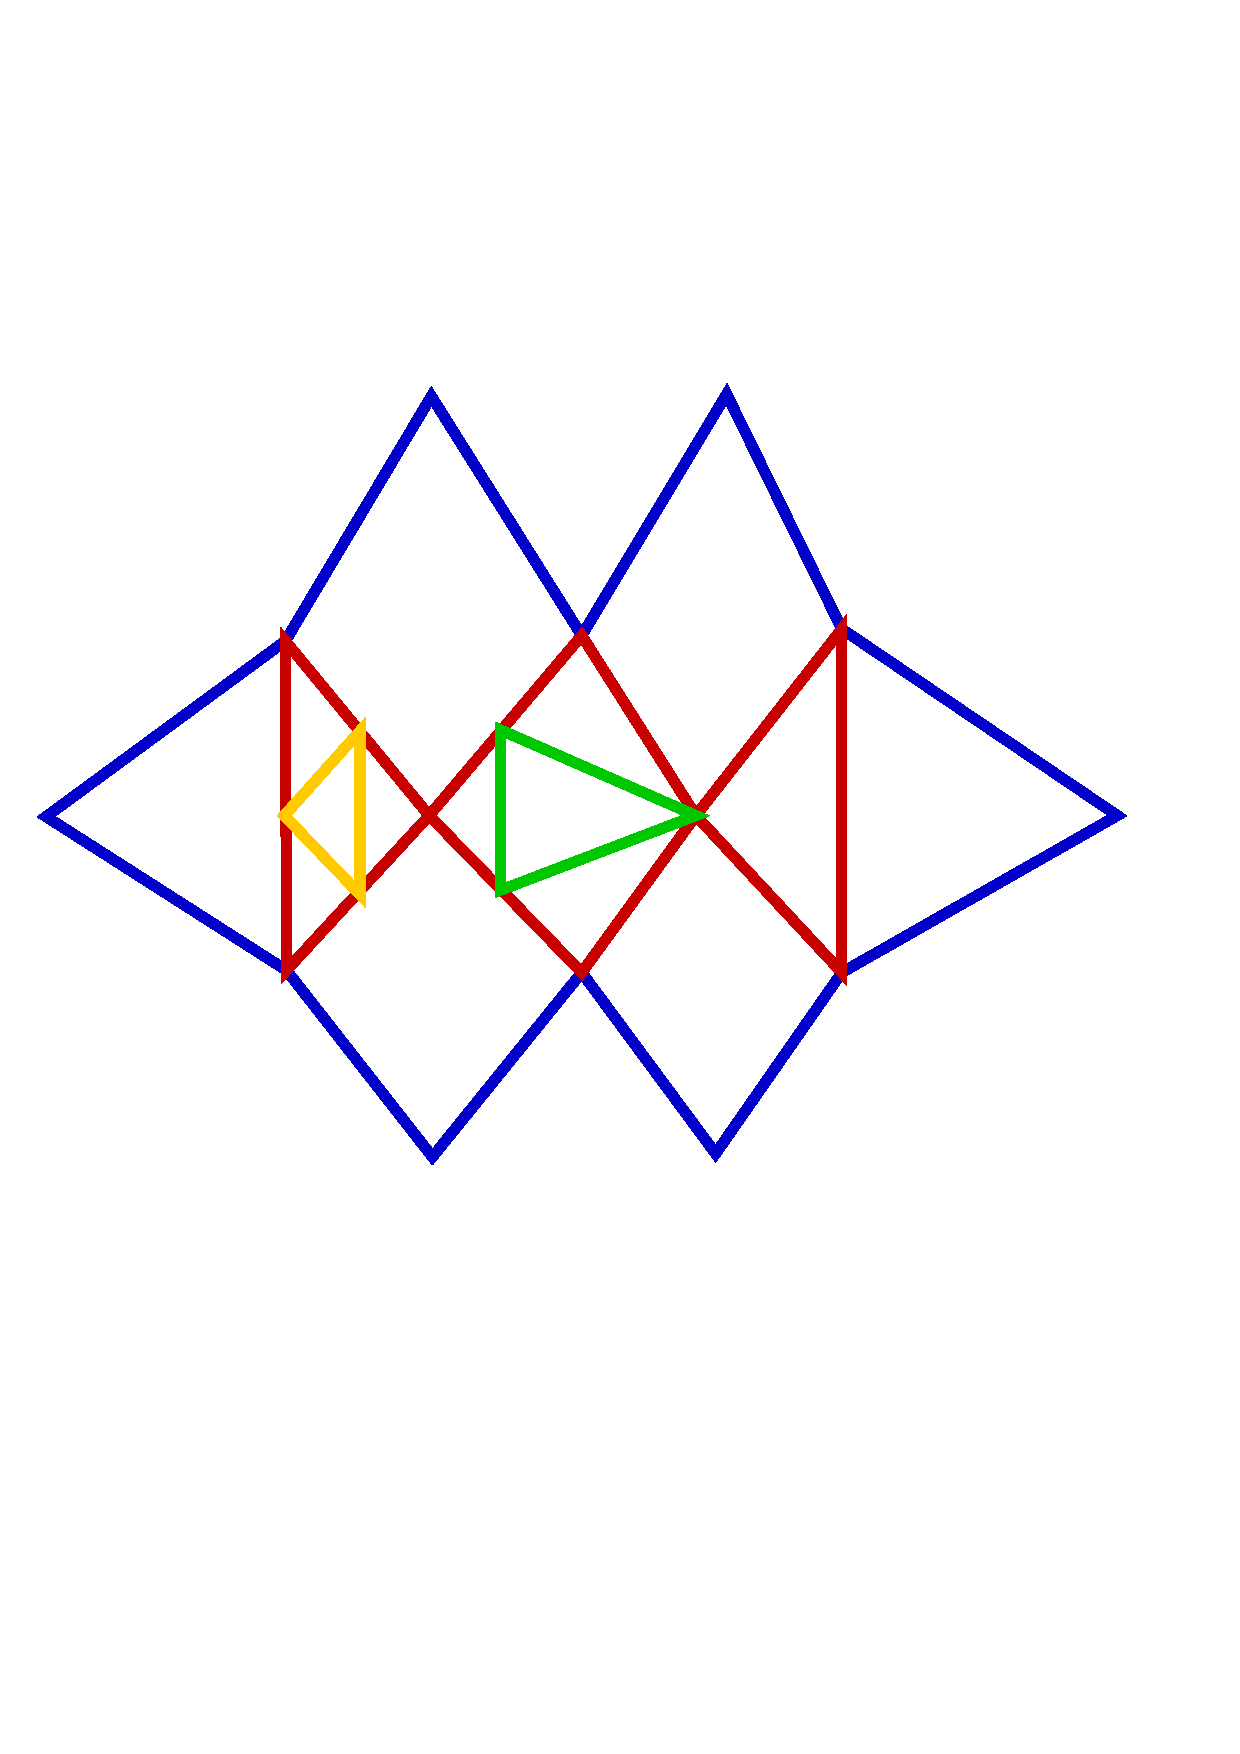
\includegraphics[scale=0.30]{cycle_tree_fig_1_crop}
	\includegraphics[scale=0.25]{cycle_tree_fig_2_crop}
        %\vspace*{-0.1in}
	\caption{
          $\tK$ (left) has $C_0$ (blue), $C_1$ (red), $C_2$ (yellow), $C_3$ (green) circuits.
          In the circuit tree (right), child circuits $C_2, C_3$  of $C_1$ are disjoint.
          %and $|C_0| \supset |C_1| \supset |C_2| \supset |C_3|$.
          }
	\label{fig:circuittree}
        \vspace*{-0.1in}
\end{figure}

Algorithm \ref{alg:circuittree} constructs the circuit tree.
It works by finding the outermost circuit in $\tK$ first, and continues to find all inner circuits in $\tK$, finishing with the innermost circuits.
The outermost circuit in the $1$-skeleton of $\tK$ consists of boundary edges in $\tK$.
An innermost circuit in the $1$-skeleton of $\tK$ contains no other circuit in its underlying space in $\tK$.  
The outermost circuit corresponds to the root node in the circuit tree, while innermost circuits are leaf nodes.
The union of all circuits in the circuit tree is $\tK$.
Every node in the Circuit tree represents a circuit.
The predecessor of a circuit $C$ (pred$(C)$) is another circuit connected to $C$ at one or more vertices.
All interior vertices in $\tK$ have even degree with at least degree $4$ (some vertices may have even degree at least $6$ due to applications of local Euler Transformation).
Some vertices at the boundary of $\tK$ may have degree $2$ as mentioned in step \ref{itm:patch} of Section \ref{subsec:clipping}.
But there is at least one boundary vertex of $\tK$ with degree at least $4$, if there is more than one node in the circuit tree.
This implies every circuit $C$ can have at most $d$ consecutive descendants in a path in the circuit tree, where $2d$ is the maximum degree of a vertex in $C$.
%since we can have $2t \leq 2m$ edges at $\tilde{v}$ belongs to same cycle in case cycle is an circuit.
Based on its construction, any two circuits in the circuit tree are disjoint if they are not on the same path starting at the root node in the circuit tree.
An example circuit tree is shown in Figure \ref{fig:circuittree}.

\medskip
Given a circuit $C_0$, the algorithm finds inner circuits as follows.
Suppose $\tf$ is a $2$-cell in $\tK$ sharing edges $\{\te_i\}$ in $C_0$ and none of its edges are marked in $\tK$ except $\{\te_i\}$.
Then all other edges of $\tf$ except $\{\te_i\}$ are part of successor circuits in the circuit tree.
Let $H$ be the collection of all the edges in all $2$-cells of the form $\tf$, except edges in $C_0$ (see Algorithm \ref{alg:findboundarycircuit}).
Then $H$ represents the next ``onion layer'' of boundary circuits.
If $C_0$ is empty, then $H$ is the  collection of all the boundary edges in $\tK$.

\smallskip
\noindent \textit{Modified Hierholzer's algorithm}: The original Hierholzer's algorithm \cite{HiWi1873} was designed for a connected graph, but in our case $H$ can have multiple components.
We want to orient the circuits in order to identify the tool path avoiding crossovers.
We assume without loss of generality that each circuit is oriented clockwise as shown in Figure \ref{fig:clockwiseeulercircuit}.
Hence subtours of this circuit are oriented clockwise as well.
Pick a vertex in $H$, find all connected subtours $\{S_j\}$ and join them to obtain a circuit.
Delete all the edges and vertices in this circuit from $H$.
Repeat the process until $H$ is empty.

\emph{Correctness:} Since the $1$-skeleton of $\tK$ is Euler, $H$ consists only of circuits, and hence Algorithm \ref{alg:findboundarycircuit} is guaranteed to terminate.
Runtime of this algorithm is $O(|E|)$, where $E$ is collection of edges in $\tK$.
%Correctness and time complexity of Cycle tree algorithm \ref{alg:cycletree} is shown below.
%\textit{Correctness:} Suppose there are some edges in $1$-skeleton of $\hat{K}$ not part of any cycle in cycle tree that implies there are vertices with odd degree. Hence proved by contradiction.\newline

\textit{Complexity:} Identification of $H$, the collection of boundary edges in $\tK$, takes $O(|E|)$ time.
For a given $H$, the modified Hierholzer's algorithm runs in $O(|E|)$ time.
and we can have at most $|E|/3$ iterations of the outermost {\bfseries while} loop in Algorithm \ref{alg:circuittree}.
Hence the circuit tree algorithm runs in $O(|E|^2)$ time.

%\input{Journal_ETWComb_Fig}

\subsection{Traversal}\label{subsec:traversal}

\begin{figure}[hbp!] 
  \centering
  %\vspace*{-0.175in}
  \includegraphics[scale=0.22]{clockwise_euler_cycle_fig_1_crop}
    %\vspace*{-0.15in}
	\caption{$C_1$ (black) of circuit tree in Figure \ref{fig:circuittree} is a circuit with clockwise orientation with no crossover is shown in pink} 
	\label{fig:clockwiseeulercircuit}
\end{figure} 

Recall that we assume all circuits are oriented clockwise.
To identify the tool path traversal that avoids crossovers, we traverse edges along the circuits in the circuit tree such that each parent and child circuit pair is traversed in opposite orientation.
Let $\tv$ be a vertex in the circuit $C_1$ that is shared by two or more circuits in the tree, and has a degree $2d$.
Then there are $q \leq d$ circuits sharing vertex $\tv$.
Further, there exists a path $P = C_1 \to C_2 \to \dots \to C_q$ in the circuit tree sharing vertex $\tv$ where $C_1$ is the ancestor and $C_q$ is the descendant of all circuits in $P$.
Orientations for all other circuits in the tree are uniquely determined, if orientation of root circuit is fixed.
We assume without loss of generality that the traversal of edges in the root circuit in $\tK$ is clockwise.

There are two types of possible subpath crossovers while traversing the circuit tree (our goal is to avoid all crossovers).
The first type of crossover is within a circuit (\textit{type-1}) and the second type of crossover occurs while traversing from a parent to a child circuit (\textit{type-2}).  
If any circuit $C_i$  of the circuit tree is traversed along its orientation (as shown in Figure \ref{fig:clockwiseeulercircuit}, for instance), then it is guaranteed that there is no subpath crossover of (\textit{type-1}).
To prevent subpath crossovers of \textit{type-2}, traverse edges of $C_i$ and pred$(C_i)$ in the circuit tree in \emph{opposite} orientations along with certain edge traversal restrictions.
In particular, the traversal of edges of $C_q$ is clockwise when $q$ is odd, else it is counterclockwise.
The tool path traversal steps are detailed below.


\begin{enumerate}
  \item\label{itm:traversrestrict}
   Let $(\te_{2j-1}, \te_{2j})$ be a pair of clockwise ordered adjacent edges on a clockwise circuit path of $C_j$, sharing vertex $\tv$.
   %Add restriction on edge traversal in $\tK$ of circuit $C_1, \dots, C_q$.
   Let $\te_i \longrightarrow \te_j$ imply we traverse $\te_j$ immediately after we traverse $\te_i$ in $\tK$.
   Add the following edge traversal restrictions in $\tK$ if $q$ is odd: $\te_1 \longrightarrow \te_{2q}, \te_{2q-1} \longrightarrow \te_{2q -3}, \te_{2q-2} \longrightarrow \te_{2q -4}, \dots,  \te_{5} \longrightarrow \te_{3},\te_{4} \longrightarrow \te_{2}$, where $\te_1 \longrightarrow \te_{2q}$ means we traverse edge $\te_1$ of cycle $C_1$ followed by $\te_{2q}$ of cycle $C_q$.
   Similarly, $\te_{2(q-i)-1} \longrightarrow \te_{2(q-i-1)-1}$ means we traverse edge $\te_{2(q-i)-1}$ of $C_{q-i}$ followed by $\te_{2(q-i-1)-1}$ of $C_{q-i-1}$ and  $\te_{2(q-i)} \longrightarrow \te_{2(q-i-1)}$  means we traverse edge $\te_{2(q-i)}$ of $C_{q-i}$ followed by $\te_{2(q-i-1)}$ of $C_{q-i-1}$.  
   If $q$ is even, we add the restrictions $\te_1 \longrightarrow \te_{2q -1},\te_{2q} \longrightarrow \te_{2q -2}, \te_{2q-3} \longrightarrow \te_{2q -5}, \dots, \te_{5} \longrightarrow \te_{3}, \te_{4} \longrightarrow \te_{2}$.
   Mark all the edges of the circuit tree on path $P$.
   An example with $q=4$ is shown in Figure \ref{fig:edgerestrictq34}.     

 \item Repeat Step \ref{itm:traversrestrict} until all the edges are marked in the circuit tree.
   
 \item Start by traversing edges of the root circuit in clockwise direction, and follow traversal restrictions.        
\end{enumerate}

\begin{figure}[htp!]
	 
	\centering
	%\includegraphics[width=43mm,height=43mm]{edge_restriction_q_3_fig_1_crop}
	%\includegraphics[width=43mm,height=43mm]{edge_restriction_q_3_fig_2_crop}	
	\includegraphics[scale=0.30]{edge_restriction_q_4_fig_1_crop}
	\includegraphics[scale=0.30]{edge_restriction_q_4_fig_2_crop}
        \medskip
	\caption{\label{fig:edgerestrictq34}
		Left figure shows a $q=4$ case, with $C_1$ (blue), $C_2$ (red), $C_3$ (green), and $C_4$ (yellow) being the only circuits in a circuit tree sharing vertex $\tv$, where $C_1$ is an ancestor and $C_4$ is descendant of all circuits in the path $p = \{C_1, C_2, C_3, C_4\}$ on the circuit tree.
		Right figure shows traversal (pink) of edges in $\tK$ of circuits $C_1, C_2, C_3, C_4$ with no crossover where $\te_1 \longrightarrow \te_7, \te_8 \longrightarrow \te_6, \te_5 \longrightarrow \te_3, \te_4 \longrightarrow \te_2$ are edge traversal restrictions.
		Traversal of edges in $C_1$ is clockwise and $C_4$ is counter-clockwise for $\tK$.}

\end{figure}


\noindent \textit{Complexity:} We examine $O(|E|)$ edges in $\tK$ for adding each edge restriction in a circuit.
Since the circuit tree can have at most $(|E|/3) - 1$ edges, the runtime of traversal restriction algorithm is $O(|E|^2)$.

\section{Effect of Extruder Size and Boundary Edges in $\tilde{K}$}\label{sec:boundaryedges}

In our related manuscript \cite{GuKr2018}, we present various measures of geometric quality of the Euler transformed complex $\hK$, and detail how the these measures could be controlled by choosing a small set of user defined parameters.
We present here a couple aspects related to the geometry of $\hK$ that is specific to 3D printing.
In particular, these aspects may affect the generation of continuous print paths.

Recall we denote by $r$ the radius of the extruder.
Depending on the infill lattice and the value of $r$, we could get discontinuous print paths as discussed below.
\begin{itemize}
   \item {\bfseries Edge Covering:}
     An edge in $\hK$ could be covered without traversing it, as shown in Figure \ref{fig:extruder_size_effect}.
     In such cases, we might not be able to generate a continuous print path even when all vertices have even degree.
     In particular, if the mitered offset by at least $r$ of a polygon in undergoes combinatorial changes, then some of its edges can be covered without actually traversing them.
     \begin{figure}[htp!] 
       \centering
       \includegraphics[width=70mm,height=50mm]{edge_coverage_effect_extruder_fig_1_crop}
       \quad
       \includegraphics[width=55mm,height=50mm]{material_collision_effect_extruder_fig_1_crop}
       \caption{
         Left: Edge $e_{ij}$ is covered by traversing edges other than $e_{ij}$ if $\norm{e_{ij}} \leq 2r + \epsilon$, where $\epsilon$ is zero or too small compared to $r$, the extruder radius.
         Right: We could get material collision if the euclidean distance $d_{ij}$ between points $i$ and $j$ is less than $2r$.}
		
       \label{fig:extruder_size_effect}
     \end{figure}
            
   \item {\bfseries Material Collision:} If the distance between any two points on nonadjacent edges is less than $2r$, we could get material collision as shown in Figure \ref{fig:extruder_size_effect}.
     In particular, if the mitered offset by at least $r$ of polygon undergoes topological changes, then traversing some of its edges can cause material collision. 
\end{itemize} 

We will assume the input complex $K$ is such that $\tK$ is not affected by extruder size in the ways outlined above. 
Still, $\tK$ could have really thin polygons due to clip (\cref{def:clip}) and patch (\cref{def:patch}) operations.
Thin polygons in $\tK$ could make the print path discontinuous in order to prevent material collision.
\begin{defn}{\label{def:shrinkable}}
  \emph{({\bfseries Shrinkable} $2$-cell with offset distance $r$)}
  Let $\tilde{f}$ is a $2$-cell in $\tilde{K}$ and $\bar{f}$ is collection of $2$-cells created after mitered $r$-offset on $\tilde{f}$. $\tilde{f}$ is shrinkable if we can apply mitered $r$-offset such that each vertex and edge in $\bar{f}$ is part of some $2$-cell in $\bar{f}$. If $\bar{f}$ has more than one   $2$-cell then it is shrinkable with topological changes. If a $2$-cell is not shrinkable then it is called unshrinkable.  
\end{defn} 

We assume the traversal of polygons in $\hK$ is not affected by the extruder size ($r$) as outlined above.
This implies interior polygons in $\hat{K}$ are not affected by the extruder size.
But traversal of edges in boundary polygons in $\tilde{K}$ may be affected by extruder size due to clip and patch operations (\cref{def:clip,def:patch}).
\cref{fig:matcola} shows possible material collision in a boundary polygon in $\tilde{K}$, since those $2$-cells become too thin and do not satisfy the assumptions in Step \ref{itm:eulertransform} on Euler Transformation.
We consider the cases where $\tilde{f}$ is shrinkable or unshrinkable based on the extruder size.  

\begin{case}
  $\tilde{f}$ is shrinkable.
\end{case}
 
If $\tilde{f}$ is shrinkable with combinatorial changes then we can print all of its edges.
But if $\tilde{f}$ is shrinkable with topological changes, then we can print only some of the edges.
Let $\tilde{f}$ is shrinkable with topological changes.
This setting also implies $\tilde{f}$ is non-convex.
Let $\tilde{v}_{k}$ be the vertex of edges $\tilde{e}, \tilde{e}'$ in $\tilde{f}$ that is split up into two vertices $\bar{v}_{k}, \bar{v}_{k+1}$ in $\bar{f}$.
Also let $v_{k}', v_{k+1}'$ be the perpendicular points of intersection through $\bar{v}_k, \bar{v}_{k+1}$ on edges $\tilde{e}, \tilde{e}'$.
Then portions of edges between $v_{k}'$ and $v_{k+1}'$ of $\tilde{e}, \tilde{e}'$ have to be set as travel paths in order to avoid material collision.
An example is shown in \cref{fig:matcol}. 

  \begin{figure}[ht!]
	\centering
	\begin{subfigure}[t]{1.4in}
		\centering
		\includegraphics[scale=0.24]{material_collision_fig_1_crop}
		\caption{\label{fig:matcola}}
	\end{subfigure}
	\hspace*{.5in}
	\begin{subfigure}[t]{1.4in}
		\centering
		\includegraphics[scale=0.24]{material_collision_updated_fig_2_crop}
		\caption{\label{fig:matcolb}}
	\end{subfigure}
	\hspace*{.5in}
	\begin{subfigure}[t]{1.4in}
		\centering
		\includegraphics[scale=0.24]{material_collision_updated_fig_3_crop}
		\caption{\label{fig:matcolc}}		
	\end{subfigure}
	\caption{\label{fig:matcol}
		Red dotted circle is extruder cross-section of radius $r$ in (a).
		$\tilde{f}$ is $2$-cell of $\tilde{K}$ created in step \ref{itm:patch} shown in (a), (b), (c).
		$\bar{f}$ is a set of $2$-cells created from $\tilde{f}$ (mitered offset), in solid blue in (b), (c).
		The set of $1$-cells created in step \ref{itm:patch} and not portion of any $1$-cell in $\hK$ is in pink.
		$\tilde{v}_1$ is original vertex of $\tilde{f}$ and $v_1', v_2'$ are perpendicular point of intersection through $\bar{v}_1, \bar{v}_2$ to corresponding edges in pink as shown in (b), (c).
		$\{v'_2, \tilde{v}_1\}$, $\{v'_1, \tilde{v}_1\}$ are travel paths in $\tilde{f}$ in (c).
	}
	%\vspace*{-0.075in}
\end{figure}

   \begin{case}
 	$\tilde{f}$ is unshrinkable
 \end{case} 
   Based on our assumptions in Step $\ref{itm:eulertransform}$ on Euler Transformation, printing all the edges or portions of those edges in $\hat{k}$ will not be affected by the extruder size ($r$).
   If $\tilde{f}$ is unshrinkable, then it will be due to boundary edges added in $\tilde{f}$, which are part of the polygon $\tilde{R}_{ij}$ used in the patch operation (\cref{def:patch}) on $\tilde{K}$ (see \cref{fig:unshrinkable}).
   These boundary edges have to be set as travel paths to avoid material collision. 
  
   \begin{figure}[htp!] 
     \centering
     %\vspace*{-0.075in}
     \includegraphics[scale=0.3]{non_shrinkable_2_cell}
     \caption{\label{fig:unshrinkable}
       Polygon $\tilde{f}$ is added to $\tilde{K}$ with the creation of edge $\tilde{e}$ in the patch step, where $\tilde{e}, \hat{e}$ are parallel with perpendicular distance $d < 2r$.
       $\tilde{f}$ is unshrinkable with offset distance $r$.
       Hence $\tilde{e}$ has to be set as a travel path.
     }
   \end{figure}

   Note that we can have at most $m/2$ boundary edges set as travel paths, when there are $m$ boundary edges on $\tilde{R}_{ij}$.

   \begin{rem}
     {\rm It is still an open problem to identify how to continuously print the boundary edges in $\tilde{K}$, if these boundary polygons  in $\tilde{K}$ are shrinkable with topological changes, or are unshrinkable.}
   \end{rem} 
\section{Discussion}\label{sec:experiment}
\vspace*{-0.1in}

The bottleneck for computational complexity of the Euler transformation is determined by the mitered offsets it creates for each cell in $K$.
The number of cells in $\hK$ are clearly linear in the number of cells in $K$ (\cref{lem:cntshVhEhF2d}).
For $d=2$, if $K$ in $\R^d$ has $m$ $d$-cells, each of which has at most $p$ facets, the time complexity of Euler transformation is $O(m p^d)$ \cite{AuWa2013,AuWa2016}.
Not all cells in the Euler transformation $\hK$ are guaranteed to be convex, even when all cells in $K$ are (see \cref{fig:disjholes}).
We could triangulate the non-convex cells so that all cells in $\hK$ are convex.
But could we do so while maintaining even degrees for all vertices?
A related problem is that of finding a triangulation (rather than a cell complex) of a given domain that minimizes the number of odd-degree vertices.
The total Euclidean length of edges is $\tilde{K}$ is going to be at least double compared to that in the original complex in $K$.
Hence it is better to start with a sparse input complex $K$ (i.e., with a smaller total Euclidean length of edges).
We have described a complete framework for continuous tool path planning in layer-by-layer 3D printing.
The clipping step will be bottlenecked by the computation of intersection of the Euler transformed complex with each polygon in each layer.
We have generalized the Euler transformation defined to allow combinatorial changes when computing mitered offsets of cells.
What about allowing topological changes?
It appears applying the generalized Euler transformation should be able to generate an Euler complex even when topological changes are allowed.
But there might be some new geometric challenges generated in this process, which would have to be taken care of.
We will address this question in future work.
Another promising generalization of our approach would be to \emph{non-planar} 3D printing.
Many of our results should generalize to the non-planar realm as long as underlying support is guaranteed by the design.